\documentclass[11pt]{article}
\usepackage[T1]{fontenc}
\usepackage{lmodern}
\usepackage[margin=1in]{geometry}
\usepackage{amsmath,amssymb,amsthm,mathtools}
\usepackage{microtype}
\usepackage{enumitem}
\usepackage{tikz}
\usetikzlibrary{arrows.meta,positioning}
\usepackage{placeins}
\usepackage{needspace}
\usepackage[hidelinks]{hyperref}
\hypersetup{pdftitle={Weak and strong normalization in pure type systems},
            pdfauthor={OpenAI}}
\newtheorem{theorem}{Theorem}
\newtheorem{lemma}[theorem]{Lemma}
\newtheorem{proposition}[theorem]{Proposition}
\newtheorem{corollary}[theorem]{Corollary}
\newtheorem{claim}{Claim}
\theoremstyle{definition}
\newtheorem{definition}{Definition}[section]
\newtheorem{remark}{Remark}[section]
\newtheorem{example}{Example}[section]
\setlist{itemsep=2pt,topsep=4pt}
\title{Weak and strong normalization in pure type systems}
\author{OpenAI}
\date{September 25, 2026}
\begin{document}
\maketitle
\begin{abstract}
We prove that every weakly $\beta$-normalizing pure type system is strongly
$\beta$-normalizing. Both properties quantify over all legal expressions
in all valid contexts, and reduction acts inside type annotations.
No functionality hypothesis is required. This resolves the
$\beta$-Barendregt--Geuvers--Klop conjecture.
\end{abstract}
\setcounter{tocdepth}{1}
\tableofcontents
\clearpage
\section{Introduction}\label{sec:introduction}

A pure type system specifies which sorts classify other sorts and which
sorts may form dependent function types.  A term is \emph{weakly
$\beta$-normalizing} if some sequence of $\beta$-reductions reaches a normal
form; it is \emph{strongly $\beta$-normalizing} if every such sequence is
finite.  The distinction is between existence of a terminating computation
and termination under every choice of reductions.

We use the full annotated syntax: reduction is allowed in the domain of
an abstraction and in both components of a dependent product. Contexts may
be open. A legal expression is either side of a derivable typing judgment;
declaration types are included by context validity. The formal rules and
conventions are given below before the main theorem.

\subsection{Pure type systems and normalization}\label{pts:setup}

We first fix the syntax and the scope of the normalization properties.
All contexts in the typing rules are finite, and all reductions include
reductions inside annotations.

\begin{definition}[Specification and expressions]\label{pts:specification}
A \emph{pure type specification} is a triple
$\mathcal P=(\mathcal S,\mathcal A,\mathcal R)$, where $\mathcal S$ is a
set of \emph{sorts}, $\mathcal A\subseteq\mathcal S^2$ is a relation of
\emph{axioms}, and $\mathcal R\subseteq\mathcal S^3$ is a relation of
\emph{product rules}. Neither relation is assumed functional.
Using a countably infinite set of variables disjoint from $\mathcal S$, form the
raw expressions
\[
 M,N,A,B ::= x\mid s\mid MN\mid\lambda x:A.M\mid\Pi x:A.B,
 \qquad s\in\mathcal S.
\]
Expressions are identified up to renaming bound variables. In each binder
the variable binds in the body or codomain, but not in its annotation or
domain. Application associates to the left. Substitution is capture
avoiding; $M[x:=N]$ denotes substitution for one free variable.

A raw context is a finite sequence
$\Gamma=(x_1:A_1,\ldots,x_n:A_n)$ with distinct declared variables.
Its domain is $\operatorname{dom}(\Gamma)=\{x_1,\ldots,x_n\}$.
Whenever a rule appends $x:A$, its variable $x$ is fresh for the preceding
context and for $A$.
\end{definition}

\begin{definition}[Full beta reduction]\label{pts:beta}
The relation $\to_\beta$ is the compatible closure of
\[
             (\lambda x:A.M)N\to_\beta M[x:=N].
\]
Compatibility permits a step in either child of an application, product,
or lambda. In particular, both
$\lambda x:A.M\to_\beta\lambda x:A'.M$ when $A\to_\beta A'$ and
$\Pi x:A.B\to_\beta\Pi x:A'.B$ are permitted.
Write $\to_\beta^*$ for its reflexive-transitive closure and
$=_\beta$ for the equivalence relation it generates. A normal expression
has no beta redex at any position. An expression is \emph{weakly
normalizing} if it reduces to a normal expression, and \emph{strongly
normalizing} if it starts no infinite reduction sequence.
\end{definition}

Typing is the least relation closed under these seven rules, with
$s,s_1,s_2,s_3$ literal sorts.
\begin{gather*}
 \frac{(s_1,s_2)\in\mathcal A}{\varnothing\vdash s_1:s_2}
 \;\textsc{Axiom}
 \qquad
 \frac{\Gamma\vdash A:s}{\Gamma,x:A\vdash x:A}
 \;\textsc{Variable}
 \\
 \frac{\Gamma\vdash M:B\qquad\Gamma\vdash A:s}
      {\Gamma,x:A\vdash M:B}
 \;\textsc{Weakening}
 \\
 \frac{\Gamma\vdash A:s_1\qquad
       \Gamma,x:A\vdash B:s_2\qquad(s_1,s_2,s_3)\in\mathcal R}
      {\Gamma\vdash\Pi x:A.B:s_3}
 \;\textsc{Product}
 \\
 \frac{\Gamma,x:A\vdash M:B\qquad\Gamma\vdash\Pi x:A.B:s}
      {\Gamma\vdash\lambda x:A.M:\Pi x:A.B}
 \;\textsc{Abstraction}
 \\
 \frac{\Gamma\vdash M:\Pi x:A.B\qquad\Gamma\vdash N:A}
      {\Gamma\vdash MN:B[x:=N]}
 \;\textsc{Application}
 \\
 \frac{\Gamma\vdash M:A\qquad\Gamma\vdash B:s\qquad A=_\beta B}
      {\Gamma\vdash M:B}
 \;\textsc{Conversion}.
\end{gather*}
The relation is understood relative to the fixed specification.
When two specifications are compared we indicate the system on the
judgment. A derivation is always finite, including a finite conversion
chain witnessing each use of $=_\beta$.

\begin{definition}[Contexts, legality, and system normalization]
\label{pts:normalization}
A context $(x_1:A_1,\ldots,x_n:A_n)$ is \emph{valid} if each $A_i$ is
typed at some literal sort in the preceding prefix. An expression is
\emph{sorted} in $\Gamma$ if $\Gamma\vdash A:s$ for some $s\in\mathcal S$.
It is \emph{legal} in $\Gamma$ if it is the subject or the expected type
of a derivable judgment in $\Gamma$.

The system is weakly normalizing, respectively strongly normalizing, if
every legal expression in every context is weakly normalizing,
respectively strongly normalizing. These are system-wide properties;
neither statement replaces its universal quantifier by a hypothesis
about a single expression. The reduction relation acts on the expression
itself, including its annotations; it does not unfold declarations in
the external context.
\end{definition}



\begin{theorem}[The $\beta$-Barendregt--Geuvers--Klop conjecture]
\label{thm:main}
Let $\mathcal P=(\mathcal S,\mathcal A,\mathcal R)$ be any pure type system.
If every legal expression of $\mathcal P$, in every valid context, is weakly
$\beta$-normalizing, then every such expression is strongly
$\beta$-normalizing. No functionality assumption is imposed on
$\mathcal A$ or $\mathcal R$.
\end{theorem}

Both quantifiers in Theorem~\ref{thm:main} range over the whole system.
The theorem does not assert that an individual term with a normal form is
strongly normalizing. In particular, the proof may use weak normalization
of expressions other than the one whose strong normalization is being
established. The result concerns $\beta$-reduction; it makes no assertion
about adding $\eta$-reduction.

\paragraph{History and significance.}
Geuvers formulates the system-wide conjecture, for both $\beta$ and
$\beta\eta$ reduction, in his thesis \cite[Conjecture~8.1.2]{Geuvers1993}.
Theorem~\ref{thm:main} establishes its $\beta$ instance for arbitrary
specifications. It allows a proof that every legal expression has a normal
form to serve also as a proof of termination under every choice of beta
reductions. This includes computations inside types and annotations,
which may continue after the computational body has reached normal form.
The hypothesis remains a property of the whole system: the argument can
use normal forms of open expressions other than the expression under study.

One line of earlier work reduces strong normalization to weak
normalization of translated terms. The translation must preserve typing,
so the products available in the source specification are decisive.
S{\o}rensen's continuation-passing construction proves the implication for
generalized nondependent, clean, negatable systems
\cite[Theorem~3.5.20]{Sorensen1997}; the uniform nondependent result of
Barthe, Hatcliff and S{\o}rensen develops this approach
\cite{BartheHatcliffSorensen2001}. Mull's thesis weakens the cleanliness
and negatability restrictions within the nondependent tiered setting
\cite[Theorem~2]{MullThesis2023}. Here the sorts form a finite axiom chain
and each product inherits its codomain's sort. In particular, the theorem
allows a weakly clean alternative at each non-top tier that does not require
negatability, alongside an alternative retaining negatability and a
further cleanliness condition. These results explain both the force of
type-preserving translations and the importance of the product rules they
require.

Structural transformations offer a complementary way to reduce the
problem. Roux and van Doorn prove weak-normalization preservation for
disjoint sums and a specified family of added product rules, using
labelled syntax and dependency erasure
\cite[Sections~3--4]{RouxVanDoorn2014}. Mull proves that the
Barendregt--Geuvers--Klop implication transfers from the irrelevance
reduction of a tiered system to that system
\cite[Theorem~47]{Mull2023}. This is a conditional reduction of the
conjecture within the tiered class. More recently, Roux proposes an
internal proof translation with reported constructions for the simply
typed lambda calculus, System~F, and a trivial recursive type
\cite[slides~16--17]{Roux2025}. The general specification considered here
need not have a hierarchy of sorts, functional axiom or product relations,
or the products required by any of these translations.

Annotations impose a separate constraint on comparisons between systems.
Barthe and Coquand exhibit nonnormalizing pure type systems in which
erasing lambda-domain annotations identifies terms of the same type and
context that are not beta-convertible
\cite[Theorem~17]{BartheCoquand2006}. The auxiliary erasure used below
retains all annotations. It removes only proof/data mode labels, and its
reduction-lifting property is proved for each ordinary typed beta step.

\paragraph{Proof strategy.}
A finite derivation of a counterexample uses only a finite part of the
specification, so the proof first reduces to finite sort and rule sets.
Under weak normalization and confluence, every legal expression then has
a unique normal form. The \emph{sort profile} of a normal type records
all sorts at which it can be typed. Retaining this set accommodates
nonfunctional specifications; tracking its growth under substitution
replaces an appeal to uniqueness of types.

The candidate argument follows the Tait--Girard reducibility tradition
\cite[Chapters~6 and~14]{Girard1989}. Its candidates are sets of strongly
normalizing terms closed under the head expansions needed here; their
lattice, product tests and substitution laws are proved explicitly,
without requiring reduction closure. Profiles form a finite signed graph:
in a dependent product, the domain reverses inclusion between candidates
and the codomain preserves it. Processing its strongly connected
components in dependency order establishes that a strongly normalizing
function applied to any finite, correctly typed stack of strongly
normalizing arguments remains strongly normalizing. This excludes a
smallest nonnormalizing application and yields the theorem.

Components whose signs are consistent admit an ordered fixed point by
Tarski's theorem \cite{Tarski1955}. A second construction handles products
with at most one child in the current component. The remaining components
require observation tables, indexed by stacks of normal arguments and
auxiliary values. Negative domain occurrences make the equations for
these spaces circular. The construction resolves that circularity using
well-founded recursion for some profiles and alternating finite stages
for the others. Its key bound is uniform over all observations of a fixed
typed expression, although the possible arguments and stack lengths are
unbounded. Semantic substitution and reduction transport then give the
candidate equality required at a dependent application.

This last construction is conditional on a graph exclusion. The forbidden
configuration records the profile pattern forced if substitution exposes
new product nodes counted by the recursion's measure on normal types.
Weak normalization rules it out through a second, typed argument. The
product rules in such a configuration support a small
formula calculus and a relational realization of Hurkens's
well-foundedness paradox \cite{Hurkens1995}, using the presentation of
Geuvers \cite[Section~2]{Geuvers2007}.

Realizing that argument requires more than reproducing its final diagonal
steps. The derived formula calculus can quantify only over data types
supported by particular product rules in the profile graph. Moreover, the
general cancellation law for wrappers compares formula observations by
logical equivalence; this gives
no permission to replace a data expression inside a function.
Two data channels provide the predicates and observations needed by the
diagonal. Their access construction retains an open parameter exactly
while rounding a second data argument. Explicit validity and
extensionality conditions then state which observations and predicates
respect the resulting comparisons. The guarded diagonal uses precisely
these conditions, and every logical quantifier is checked against the
available product rules.

The resulting labelled term proves a designated terminal formula in a
context where a direct syntactic descent excludes every proof-mode term
with normal erasure. Data inhabitants of the same terminal do not affect
this statement. Erasure leaves all type annotations intact, and every
ordinary reduction of the erased typed proof lifts to a labelled
reduction. Weak normalization would therefore give the excluded normal
erasure. This contradiction supplies the graph exclusion and completes
the candidate argument.

\paragraph{Organization.}
Section~\ref{pts:metatheory} establishes the required PTS metatheory.
Sections~\ref{sec:profiles} and~\ref{sec:simple-components} develop the
candidate interface and its two simpler realizations.
Section~\ref{obs:section} constructs the remaining interpretation,
conditional on the graph exclusion. Sections~\ref{sec:enc-wrappers},
\ref{chan-section} and~\ref{rel-section} build the logical and relational
realization. Section~\ref{rel-diagonal} gives the guarded diagonal
argument. Section~\ref{sec:conclusion} proves the exclusion and completes
the theorem.


\section{Structural properties}\label{pts:metatheory}

The following facts let us use finite open contexts and chosen typing
derivations without assuming uniqueness of sorts or product rules.
These are standard properties of pure type systems; compare
\cite[Chapter~2]{Poll1994}. We give the proofs needed here, especially the
steps concerning annotations and nonfunctional specifications.

\begin{lemma}[Validity and scope]\label{pts:validity}
If $\Gamma\vdash M:A$, then $\Gamma$ is valid, and
$\mathrm{FV}(M)\cup\mathrm{FV}(A)\subseteq\operatorname{dom}(\Gamma)$.
For each declaration of $\Gamma$, its sorting judgment in the preceding
prefix occurs as a subderivation of the given derivation.
\end{lemma}

\begin{proof}
Induct on the derivation. An axiom has empty context. The variable and
weakening rules supply the sorting judgment for their last declaration;
the induction hypothesis supplies the earlier ones. Every other rule
has a premise with unchanged context, so its induction hypothesis
supplies validity and the required subderivations. Scope follows in the
same induction. For application, use
\[
 \mathrm{FV}(B[x:=N])\subseteq
       (\mathrm{FV}(B)\setminus\{x\})\cup\mathrm{FV}(N).
\]
The binder cases remove their fresh bound variable from the free
variables of the body.
\end{proof}

\begin{lemma}[Thinning by insertion]\label{pts:thinning}
Suppose $\Gamma\vdash M:A$, and suppose that $\Delta$ is a valid context
containing the declarations of $\Gamma$ unchanged and in their original
order. Then $\Delta\vdash M:A$.
\end{lemma}

\begin{proof}
Induct on the size of the given derivation. For an axiom, weaken through
the declarations of $\Delta$. For a variable or weakening rule, split
$\Delta$ just after the last declaration of the source context.
Transport the rule's premises to the part before that declaration by
induction, reapply the rule, and then weaken through the remaining
suffix. The necessary sorting judgments for that suffix are supplied
by validity of $\Delta$.

At a binder, first rename its bound variable fresh for $\Delta$.
Its domain sorting is a premise of product formation or a smaller
subderivation supplied by Lemma~\ref{pts:validity}. Induction transports
this sorting to $\Delta$, making the extended target context valid.
Induction therefore also transports the body or codomain premise to
that extension. Reapply the original rule. Application and conversion
transport their unchanged-context premises and reapply their rule.
\end{proof}

\begin{lemma}[Typed substitution]\label{pts:substitution}
Let $\Gamma=(x_1:A_1,\ldots,x_n:A_n)$ and let $\Delta$ be valid.
Suppose a simultaneous substitution $\sigma$ satisfies
\[
 \Delta\vdash\sigma(x_i):A_i[\sigma|_{\{x_1,\ldots,x_{i-1}\}}]
 \qquad(1\leq i\leq n).
\]
Then $\Gamma\vdash M:A$ implies $\Delta\vdash M\sigma:A\sigma$.
In particular, if
\[
 \Gamma,x:D,\Theta\vdash M:A,
 \qquad \Gamma\vdash N:D,
\]
then
\[
 \Gamma,\Theta[x:=N]\vdash M[x:=N]:A[x:=N].
\]
\end{lemma}

\begin{proof}
Raw substitution preserves beta conversion. Indeed, a substituted root
contraction is a contraction after renaming bound variables fresh;
the required equality is the composition law for capture-avoiding
substitutions. Compatibility extends this to every reduction position,
and hence to conversion chains.

For the simultaneous assertion, induct on the source derivation.
Thin axioms to $\Delta$. At a variable use its assigned judgment, and
at weakening discard the assignment for the last declaration. Under a
binder $x:D$, choose $y$ fresh for $\Delta$ and the images of $\sigma$.
Transport the domain sorting by induction, extend the target context
to $\Delta,y:D\sigma$, and extend the substitution by $x\mapsto y$.
The earlier assignments thin to this context; the new assignment is
the variable rule. Apply induction to the binder premise and reapply
product formation or abstraction with the original axiom or rule
choices. Application uses substitution composition. Conversion uses
the transported sorting of its target and preservation of raw
conversion.

For single substitution with a dependent suffix, construct the target
context one declaration at a time. Start with the identity assignments
on $\Gamma$ and the image $x\mapsto N$. Transport the first suffix
declaration's sort judgment by the simultaneous assertion, append that
declaration, thin the old assignments, and assign its new variable to
itself. Repeat through $\Theta$, then transport the desired judgment.
This also proves validity of the substituted target context.
\end{proof}

\begin{lemma}[Conversion of a declaration]\label{pts:context-conversion}
Suppose $\Gamma\vdash D:s$, $\Gamma\vdash D':s'$, and $D=_\beta D'$.
Replacing $x:D$ by $x:D'$ in any valid context
$\Gamma,x:D,\Theta$ preserves validity and every derivable judgment,
with the subject, expected type, and later declarations unchanged.
The converse replacement has the same property.
\end{lemma}

\begin{proof}
In $\Gamma,x:D'$ the variable rule gives $x:D'$. Thin the old sorting
of $D$ to this context and convert to obtain $x:D$. Thus the identity
on the old variables is a typed substitution from $\Gamma,x:D$ to
$\Gamma,x:D'$. As in the suffix construction in
Lemma~\ref{pts:substitution}, transport each later sorting judgment,
append the same declaration, and extend the identity substitution.
Finally transport the desired judgment. Interchanging $D,D'$ proves
the reverse assertion. Nothing requires $s=s'$.
\end{proof}

\Needspace{4\baselineskip}
\begin{lemma}[Generation]\label{pts:generation}
For derivable judgments in an arbitrary pure type system:
\begin{enumerate}
\item If $\Gamma\vdash x:T$, then $x:D$ occurs in $\Gamma$ and
      $T=_\beta D$.
\item If $\Gamma\vdash s:T$, then $(s,u)\in\mathcal A$ and
      $T=_\beta u$ for some sort $u$.
\item If $\Gamma\vdash\Pi x:D.E:T$, then for some
      $(a,b,c)\in\mathcal R$,
      \[
       \Gamma\vdash D:a,\qquad
       \Gamma,x:D\vdash E:b,\qquad T=_\beta c.
      \]
\item If $\Gamma\vdash\lambda x:D.M:T$, then for some $E,c$,
      \[
       \Gamma,x:D\vdash M:E,\qquad
       \Gamma\vdash\Pi x:D.E:c,\qquad
       T=_\beta\Pi x:D.E.
      \]
\item If $\Gamma\vdash MN:T$, then for some $D,E,x$,
      \[
       \Gamma\vdash M:\Pi x:D.E,\qquad
       \Gamma\vdash N:D,\qquad T=_\beta E[x:=N].
      \]
\end{enumerate}
Every immediate syntactic child of a typable expression is typable
in the corresponding context, with a binder declaration added for a
body or codomain.
\end{lemma}

\begin{proof}
Induct on the derivation, stripping any final conversion and weakening
steps. Conversion composes the asserted conversion of expected types.
For weakening, thin all extracted premises back to the original
context, including under a fresh binder. When neither rule is last,
the outer syntax identifies its introducing rule and supplies the
displayed premises. The child assertion follows from these premises;
for a lambda's annotation use validity of the body context.
\end{proof}

\begin{lemma}[Correctness of types]\label{pts:correctness}
If $\Gamma\vdash M:A$, then either $A$ is a literal sort or
$\Gamma\vdash A:s$ for some sort $s$. Moreover, every type assigned
to an application is sorted, including an assigned type that is itself
a literal sort. Consequently every nonliteral legal expression is
typable.
\end{lemma}

\begin{proof}
Induct on the derivation. The axiom and product conclusions have literal
sorts as expected types. Variable, weakening, abstraction, and conversion
use their sorting premises, thinning where necessary. In the application
case, induction on the function premise sorts its product type, since
that type is not a literal sort. Product generation then gives a sorting
of the codomain under the binder. Substitution sorts the instantiated
result type. This also proves the stronger application assertion at
a direct application rule; final weakening preserves it by thinning,
and final conversion explicitly sorts the new expected type. Every
legal expression that occurs as an expected type is therefore either
typable or a literal sort.
\end{proof}

\subsection{Conversion and preservation of typing}
\label{pts:reduction-metatheory}

The next lemma concerns raw expressions. Thus it applies before any
normalization assumption, regardless of which products a specification
can form.

\begin{lemma}[Confluence and product compatibility]\label{pts:confluence}
Full beta reduction on raw expressions is confluent. Therefore distinct
sorts are not convertible, no product is convertible to a sort, and
\[
 \Pi x:D.E=_\beta\Pi x:D'.E'
 \quad\Longrightarrow\quad
 D=_\beta D'\ \hbox{ and }\ E=_\beta E',
\]
after consistently renaming the bound variables.
\end{lemma}

\begin{proof}
Define parallel contraction $\Rightarrow$ by reflexive variable and
sort clauses, homomorphic clauses for all expression constructors, and
the additional clause
\[
 \frac{D\Rightarrow D'\qquad M\Rightarrow M'\qquad N\Rightarrow N'}
      {(\lambda x:D.M)N\Rightarrow M'[x:=N']}.
\]
In particular the homomorphic binder clauses reduce both children.
Induction on a parallel derivation proves parallel substitution:
if $M\Rightarrow M'$ and $N\Rightarrow N'$, then
$M[x:=N]\Rightarrow M'[x:=N']$. For its contracting case, rename
the contracted binder fresh and use composition of substitutions;
the other cases reapply the corresponding homomorphic clause.

Define $M^*$, its complete development, recursively by developing every
child, with
\[
 ((\lambda x:D.P)Q)^*=P^*[x:=Q^*]
\]
at an application whose original function is a lambda. At any other
application use $(PQ)^*=P^*Q^*$. We claim that
$M\Rightarrow N$ implies $N\Rightarrow M^*$. Prove this by induction
on the parallel derivation. At an original root redex, either the
first parallel step was homomorphic, in which case contract the root
in the second step, or it contracted the root, in which case parallel
substitution applies. At an original nonredex application, use the
homomorphic clause in the second step, even if its function has become
a lambda. The remaining cases follow by the corresponding
homomorphic clauses and induction. Thus any two parallel reducts of
$M$ parallel-reduce to $M^*$, proving the diamond property.

Every ordinary step is parallel. Conversely, every parallel step is
a finite sequence of ordinary steps: first reduce the children and
then perform its root contraction, if any. Hence the reflexive-transitive
closures of the two relations coincide, and beta reduction is confluent.
Convertible expressions consequently have a common reduct. Reducing
a product never removes its outer constructor, whereas a sort is
irreducible. Comparing the common reducts gives all the asserted
compatibility and separation properties.
\end{proof}

\begin{lemma}[Subject reduction]\label{pts:subject-reduction}
If $\Gamma\vdash M:A$ and $M\to_\beta^*M'$, then
$\Gamma\vdash M':A$, with the exact original expected type.
\end{lemma}

\begin{proof}
It suffices to consider one step. Induct on the typing derivation.
There are no steps from sorts or variables. At a final weakening or
conversion, apply induction to its subject premise and reapply the
same rule.

At product formation, a step in the domain preserves its original sort
by induction. Lemma~\ref{pts:context-conversion} transports the codomain
sorting to the changed binder context, and the same product rule
re-forms the result. A codomain step is handled by induction on its
typing premise.

At abstraction, a step in the body is immediate by induction. For an
annotation step $D\to_\beta D'$, the supporting judgment
$\Gamma\vdash\Pi x:D.E:c$ is a strictly smaller premise derivation.
Apply induction to its corresponding domain step to get
$\Gamma\vdash\Pi x:D'.E:c$. Product generation sorts $D'$;
context conversion then transports the body judgment to
$\Gamma,x:D'$. Abstraction gives the changed lambda its new product
type. Convert back to the old product type, which is sorted by the
original supporting premise.

At application, a step in the function preserves its product type by
induction. A step $N\to_\beta N'$ in the argument gives the new
result type $E[x:=N']$; convert this to $E[x:=N]$, whose sorting was
proved in Lemma~\ref{pts:correctness}.

It remains to treat a root contraction
$(\lambda x:D_0.P)N\to_\beta P[x:=N]$. Suppose the application
premises assign the function type $\Pi x:D.E$ and the argument
type $D$. Generation of the function judgment gives some $E_0,c$
such that
\[
 \Gamma,x:D_0\vdash P:E_0,
 \qquad\Gamma\vdash\Pi x:D_0.E_0:c,
 \qquad\Pi x:D_0.E_0=_\beta\Pi x:D.E.
\]
Product compatibility gives $D_0=_\beta D$ and $E_0=_\beta E$.
Generation of the supporting product sorts $D_0$, so convert
$N:D$ to $N:D_0$. Substitution yields
$\Gamma\vdash P[x:=N]:E_0[x:=N]$.
Convert to the old application type $E[x:=N]$, which is sorted by
Lemma~\ref{pts:correctness}. This completes every reduction position,
including positions inside annotations.
\end{proof}

\subsection{Neutral expressions and normal forms}
\label{pts:neutrals}

An expression $xN_1\cdots N_k$, with $k\geq0$, is called
\emph{neutral}. Its arguments need not be normal. This restricted
class has unique types even when the specification does not.

\begin{lemma}[Uniqueness for neutral expressions]\label{pts:neutral-uniqueness}
If $H$ is neutral and $\Gamma\vdash H:A$ and $\Gamma\vdash H:B$,
then $A=_\beta B$. If $\Gamma\vdash H:s$ for a literal sort $s$,
then $s$ itself is sorted in $\Gamma$. Every normal typable application
is neutral.
\end{lemma}

\begin{proof}
Induct on the length of the neutral spine. At a variable, generation
identifies both types with its declaration type up to conversion.
For $HN$, generation of its two typings gives function product types
$\Pi x:D.E$ and $\Pi x:D'.E'$. Induction makes these convertible.
Product compatibility gives $E=_\beta E'$, so substitution makes
their instantiated codomains convertible. These codomains are
convertible to the original two result types by generation.

If a variable has type $s$, its declaration type $D$ is sorted by
validity and thinning, and $D=_\beta s$ by generation. Confluence
and irreducibility of $s$ give $D\to_\beta^*s$. Subject reduction
therefore sorts $s$. For a nonempty neutral spine, the stronger
application assertion in Lemma~\ref{pts:correctness} sorts its
expected type directly.

Finally, the head of a normal application cannot be a lambda, since
that would give a redex. It cannot be a sort or product: generation
makes any type of either head convertible to a sort, whereas the
first application requires a product type. Product/sort separation
excludes this. The only remaining head is a variable.
\end{proof}

\begin{remark}\label{pts:nonfunctionality}
General uniqueness of types is false under our hypotheses. For example,
if $(r,a)$ and $(r,b)$ are axioms with distinct $a,b$, then $r$ has
the two nonconvertible types $a,b$. Lemma~\ref{pts:neutral-uniqueness}
does not apply to the sort $r$. No later use of uniqueness concerns
an arbitrary expression.
\end{remark}

\begin{lemma}[Normalizing judgments]\label{pts:normalizing-judgments}
Assume that every legal expression is weakly normalizing. Write
$M^\#$ for its normal form, uniquely determined up to alpha equivalence.
If $\Gamma\vdash M:A$, then
\[
                \Gamma\vdash M^\#:A
                \qquad\text{and}\qquad
                \Gamma\vdash M^\#:A^\#.
\]
The second judgment is also available with $M$ in place of $M^\#$.
If $\Gamma\vdash A:s$, then $\Gamma\vdash A^\#:s$.
A sorted normal expression is either a sort, a neutral expression,
or a product.
\end{lemma}

\begin{proof}
Weak normalization supplies normal forms; confluence gives uniqueness.
Subject reduction proves the first judgment and the assertion about
sorting. Correctness of types says that $A$ is sorted or is a literal
sort. In the first case subject reduction sorts $A^\#$, allowing
conversion of the expected type. In the second case $A^\#=A$, so
there is nothing to convert if that sort is unsorted. Finally a
normal application is neutral by Lemma~\ref{pts:neutral-uniqueness},
and a lambda cannot have a sort type by generation and product/sort
separation.
\end{proof}

\subsection{Finite specifications and a common context}
\label{pts:finite-and-context}

For the main implication it is enough to work with a finite
specification. We will then place all finite contexts inside one
countable context, while each judgment continues to use only a finite
prefix.

\begin{lemma}[Finite restriction]\label{pts:finite-restriction}
Let $\mathcal P=(\mathcal S,\mathcal A,\mathcal R)$ be a pure type
system.  An expression is called \emph{legal} if it occurs as the subject
or the expected type of a derivable judgment.  If every legal expression
of $\mathcal P$ is weakly normalizing for full $\beta$-reduction, but some
legal expression is not strongly normalizing, then there are finite sets
\[
  \mathcal S_0\subseteq\mathcal S,\qquad
  \mathcal A_0\subseteq\mathcal A\cap\mathcal S_0^2,\qquad
  \mathcal R_0\subseteq\mathcal R\cap\mathcal S_0^3
\]
such that the restricted system
$\mathcal P_0=(\mathcal S_0,\mathcal A_0,\mathcal R_0)$ has the same two
properties.
\end{lemma}

\begin{proof}
First recall how legality relates to typability.  If $E$ is a subject,
it is typable by definition.  If $E$ is an expected type, correctness of
types says that either $E$ is a literal sort or $\Gamma\vdash E:s$ for
some context $\Gamma$ and sort $s$.  Thus every nonliteral legal
expression is typable.  Also, context validity says that each declaration
type is sorted in its preceding context, so declaration types introduce
no further kind of untypable expression.  Literal sorts have no
$\beta$-redexes.

Choose a legal expression $E$ that is not strongly normalizing.  It is
not a literal sort, so fix a finite derivation of a judgment
$\Gamma\vdash E:B$.  For every use of conversion in this derivation,
choose a finite raw $\beta$-conversion chain witnessing its side
condition.  Let $\mathcal S_0$ contain all sorts occurring in the
derivation and these chains.  Let $\mathcal A_0$ and $\mathcal R_0$
contain the axiom pairs and formation triples used in the derivation,
enlarging $\mathcal S_0$ to contain their entries if necessary.  These
sets are finite, and the same derivation and conversion chains establish
$\Gamma\vdash E:B$ in $\mathcal P_0$.

A full $\beta$-step introduces no new sort symbol: substitution can only
copy symbols already present in the redex, and contextual reduction has
the same property, including reduction in annotations.  Consequently
the infinite reduction from $E$ witnessing failure of strong
normalization is also a reduction in the raw syntax over
$\mathcal S_0$.

Conversely, every judgment derivable in $\mathcal P_0$ is derivable in
$\mathcal P$.  If $F$ is legal in $\mathcal P_0$, the weak-normalization
hypothesis therefore supplies a finite reduction $F\to_\beta^*N$ in
$\mathcal P$ with $N$ normal.  No term in this reduction contains a sort
outside $\mathcal S_0$.  The reduction is thus available in
$\mathcal P_0$, and normality is unchanged, since it is the absence of a
syntactic $\beta$-redex.  This proves weak normalization of every legal
expression of $\mathcal P_0$, while $E$ remains a legal expression that
is not strongly normalizing.
\end{proof}

\begin{lemma}[A saturated context]\label{pts:saturated-context}
Suppose that the sort set $\mathcal S$ is at most countable, and that
the variable set is countably infinite.  There is a possibly empty
countable sequence of declarations $\Omega$ with the following
properties.  A judgment over $\Omega$ means a judgment derivable over
some finite initial segment of $\Omega$.
\begin{enumerate}
\item Every finite initial segment of $\Omega$ is valid.  An infinite
set of variable names is disjoint from all its declared names.
\item If $P$ is a finite initial segment of $\Omega$ and
$P\vdash D:s$, then $\Omega$ contains infinitely many declarations
$y:D$ after $P$, with distinct declared names.
\item Every finite valid context embeds, by an injective renaming of
its declared variables, as a subsequence of a finite initial segment
of $\Omega$.  If $\Gamma\vdash M:A$, such an embedding $\rho$ gives
$P\vdash M\rho:A\rho$ for a finite initial segment $P$ containing the
embedded context.
\item If $P\vdash D:s$ for a finite initial segment $P$, and $F$ is any
finite set of variable names, there is a larger finite initial segment
$Q$ ending in a declaration $y:D$, where
$y\notin F\cup\operatorname{dom}(P)$, and $Q\vdash y:D$.
\end{enumerate}
Moreover, finitely many judgments over $\Omega$ hold over a common
finite initial segment.  Injective renaming in the third clause
preserves and reflects weak and strong normalization.
\end{lemma}

\begin{proof}
Partition the variable names into disjoint infinite sets $V_0$ and
$V_1$.  Only names in $V_0$ will be declared in $\Omega$; names in
$V_1$ remain available for bound variables.  Because $\mathcal S$ and
the variable set are countable, the set of finite raw expressions is
countable.  We work up to $\alpha$-equivalence, or equivalently choose
representatives when enumerating expressions.

Choose a sequence of pairs $(p,D)$, with $p$ a nonnegative integer and
$D$ a raw expression, in which every pair occurs infinitely often.
Construct finite contexts $\Delta_n$ starting with the empty context.
At stage $n$, consider the scheduled pair $(p,D)$.  If $\Delta_n$ has
at least $p$ declarations and its initial segment of length $p$ derives
$D:s$ for some sort $s$, append a declaration $y:D$, choosing
$y\in V_0\setminus\operatorname{dom}(\Delta_n)$.  Otherwise leave
$\Delta_n$ unchanged.  This is a set-theoretic construction and does
not require a decision procedure for typing.  In the append case,
scope gives $\mathrm{FV}(D)\subseteq
\operatorname{dom}(\Delta_n)$, and thinning gives
$\Delta_n\vdash D:s$.  Thus the new declaration is fresh and the
extended context is valid.  Induction proves validity at every stage.

Let $\Omega$ be the sequence obtained by retaining all declarations
appended in this construction.  Every finite initial segment appears
at some stage and is valid.  No name from $V_1$ is declared.  If
$P\vdash D:s$ and $P$ has length $p$, then, once $P$ has been
constructed, every later occurrence of the pair $(p,D)$ appends a new
declaration of type $D$.  There are infinitely many such occurrences.
This proves the first two clauses, including the case where no
declaration is ever possible and $\Omega$ is empty.

For the embedding clause, write a finite valid context as
\[
  \Gamma=(x_1:D_1,\ldots,x_m:D_m).
\]
Induct on its prefixes.  Suppose an injective renaming $\rho_i$ embeds
the first $i$ declarations, in their original order, into a finite
initial segment $P_i$ of $\Omega$.  Validity supplies
\[
  x_1:D_1,\ldots,x_i:D_i\vdash D_{i+1}:s
\]
for some sort $s$.  Renaming and then thinning yield
$P_i\vdash D_{i+1}\rho_i:s$.  By the second clause, a later
declaration has the form $y:D_{i+1}\rho_i$, with $y$ fresh for the
already chosen names.  Set $\rho_{i+1}(x_{i+1})=y$ and take an initial
segment through this declaration.  This retains all previously
embedded declarations unchanged and in order.  The induction begins
with the empty context and proves the desired embedding.

Renaming a derivation gives
$\Gamma\rho\vdash M\rho:A\rho$.  The chosen initial segment is a
valid extension by insertion of $\Gamma\rho$, so thinning gives the
asserted judgment over that initial segment.  All substitutions and
renamings here are capture-avoiding; the reserved names permit bound
variables to be renamed away from the declarations whenever needed.

For the fourth clause, only finitely many of the infinitely many
declarations of type $D$ after $P$ can have their declared names in
$F$.  Choose any other one and let $Q$ be the initial segment ending
there.  Thinning the judgment for $D$ to the prefix immediately before
that declaration, followed by the variable rule, gives $Q\vdash y:D$.
In particular, when finitely many substitution images have their free
variables in $P$, this $y$ is fresh for all those images.

Finally, take the longest among finitely many initial segments
witnessing judgments over $\Omega$ and thin all the judgments to it.
An injective renaming of the finitely many variables of a context can
be extended to a bijective renaming of the whole variable set.  Such
a renaming commutes with full $\beta$-reduction and its inverse does
too.  It therefore preserves and reflects normal forms, finite
normalizing reductions, and infinite reductions.  This proves the
last assertions.
\end{proof}


\section{Sort profiles and normalization candidates}
\label{sec:profiles}

Throughout this section the pure type specification is finite and every
legal expression is weakly normalizing for full beta reduction. We use
the substitution, generation, context-conversion, subject-reduction and
confluence properties established in the preliminaries. Write $M^\#$
for the normal form of a legal expression, up to alpha conversion.
In particular, the expected type of a judgment has a normal form: it is
either sorted or already a literal sort. No uniqueness of sorts or
product rules is assumed.

We first associate a finite set of sorts to each type. These sets will
order the normalization argument. Within one part of that order we
shall construct sets of terms that pass certain application tests. The
main result of the section is an interface theorem: any construction
with the specified substitution and product properties advances the
normalization argument by one component.

\subsection{Profiles and the dependency graph}

For a sort $s$ and sets of sorts $I,J$, put
\[
 \operatorname{Ax}(s)=\{t:(s,t)\in\mathcal A\},\qquad
 \operatorname{Out}(I,J)
 =\{c:\text{some }a\in I,\ b\in J\text{ satisfy }(a,b,c)\in\mathcal R\}.
\]
For an expected type $T$ in a valid context $\Gamma$, define its
\emph{profile} by
\[
             \pi_\Gamma(T)=\{s:\Gamma\vdash T^\#:s\}.
\]
The profile can be empty when $T$ is an unsorted literal sort. When the
context is clear we omit its subscript. A \emph{neutral expression} is
a variable followed by zero or more arguments.

\begin{lemma}[Normal profiles]
\label{lem:normal-profiles}
A sorted normal expression is a sort, a neutral expression, or a
product. Its profile is determined as follows:
\begin{enumerate}
\item a literal sort $s$ has profile $\operatorname{Ax}(s)$;
\item a neutral expression has a singleton profile $\{s\}$, and
      $\operatorname{Ax}(s)$ is nonempty;
\item a normal product $\Pi x:D.E$ has profile
\[
 \operatorname{Out}\bigl(\pi_\Gamma(D),
                         \pi_{\Gamma,x:D}(E)\bigr).
\]
\end{enumerate}
Profiles are unchanged by valid thinning and context conversion.
If $\xi:\Gamma\to\Delta$ is a typed substitution, then
\begin{equation}
                  \pi_\Gamma(T)
                    \subseteq\pi_\Delta(T\xi).
\label{eq:profile-growth}
\end{equation}
\end{lemma}

\begin{proof}
A normal application is variable-headed: a lambda head would be a
redex, and a sort or product cannot have a product type by generation
and product compatibility. A lambda cannot have a literal sort type
for the same reason. Generation for a sort gives exactly its axiom
targets. Generation and product formation give the two inclusions in
the formula for a product, separately for every applicable rule.

For a neutral expression, its type is unique up to conversion. Indeed,
the assertion for its head variable follows from its declaration.
Inductively, generation and compatibility of convertible products
identify the domain and instantiated codomain at each further
application. Thus two literal sort types of a neutral are identical.
Its literal sort type $s$ is itself sorted. For a lone variable its
declaration type is sorted and convertible to $s$; confluence makes
that declaration type reduce to $s$, and subject reduction sorts $s$.
For a nonempty application spine, correctness of the expected type
already gives a sorting of $s$. Generation for $s$ now implies
$\operatorname{Ax}(s)\ne\varnothing$.

Thinning preserves the profile by induction on normal syntax. At a
neutral, an existing sort is retained and uniqueness excludes any new
one. At a product apply the induction also in its extended binder
context. Literal sorts do not depend on the context. Context conversion
preserves all relevant judgments in both directions, hence preserves
profiles as well.

Finally, if $s\in\pi_\Gamma(T)$, substitution gives
$\Delta\vdash T^\#\xi:s$. Reduction of $T$ to $T^\#$ commutes with
substitution, so $T^\#\xi$ and $T\xi$ have the same normal form.
Subject reduction therefore gives
$\Delta\vdash(T\xi)^\#:s$. This proves the inclusion. For a
substituted product the outer product persists, and its components
normalize separately; context conversion transports the open
codomain to the normalized domain. The same inclusion consequently
holds at corresponding product children.
\end{proof}

A nonempty profile is \emph{feasible} if it occurs in some valid
context. Since the specification is finite, there are only finitely
many feasible profiles.

\begin{lemma}[Feasible profiles]
\label{lem:feasible-profiles}
The feasible profiles form the smallest family containing
\[
 \operatorname{Ax}(s)\quad\hbox{and}\quad\{s\}
       \qquad\bigl(\operatorname{Ax}(s)\ne\varnothing\bigr)
\]
and closed under nonempty values of $\operatorname{Out}$.
\end{lemma}

\begin{proof}
Necessity follows by induction on a sorted normal expression, using
Lemma~\ref{lem:normal-profiles}. Conversely, $s$ witnesses
$\operatorname{Ax}(s)$, and a variable declared at type $s$ witnesses
$\{s\}$. Given normal witnesses for $I$ and $J$, rename their finite
contexts apart and combine those contexts by thinning. Form a product
with the first witness as domain and the second as a codomain
independent of its fresh binder. Its profile is exactly
$\operatorname{Out}(I,J)$. These witnesses are normal.
\end{proof}

Call $(I,J,K)$ a \emph{profile triple} when $I,J,K$ are feasible and
$K=\operatorname{Out}(I,J)$. Define the \emph{primary graph}, a finite signed directed graph on
the feasible profiles, by adding:
\begin{itemize}
\item a positive edge $L\to J$ whenever $L\supsetneq J$;
\item for each profile triple $(I,J,K)$, a negative edge $I\to K$
      and a positive edge $J\to K$.
\end{itemize}
Parallel edges retain their signs and their associated triples. Here and
below a path means a finite directed walk: vertices and edges may repeat.
Its parity is the parity of its number of negative edges; a
length-zero path is even.

If $T=\Pi x:D.E$ has profile $K$, write $I=\pi(D)$ and
$J=\pi(E)$. For every typed $n:D$, profile growth gives
\begin{equation}
 L=\pi\bigl((E[x:=n])^\#\bigr)\supseteq J,
 \qquad L\longrightarrow J\longrightarrow K
 \quad\hbox{by positive edges},
\label{eq:codomain-ascent}
\end{equation}
where the first edge is omitted when $L=J$.

\begin{figure}[ht]
\centering
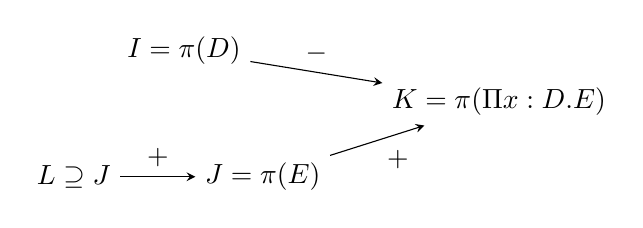
\begin{tikzpicture}[>=stealth,baseline=(current bounding box.center)]
\node (I) at (0,1.1) {$I=\pi(D)$};
\node (L) at (-1.4,-.5) {$L\supseteq J$};
\node (J) at (1,-.5) {$J=\pi(E)$};
\node (K) at (4,.45) {$K=\pi(\Pi x:D.E)$};
\draw[->] (I) -- node[above] {$-$} (K);
\draw[->] (J) -- node[below right] {$+$} (K);
\draw[->] (L) -- node[above] {$+$} (J);
\end{tikzpicture}
\caption{The domain and open codomain point to their product. An
instantiated codomain has profile $L\supseteq J$ and also has a
positive path to the product. The edge $L\to J$ is omitted if $L=J$.}
\label{fig:profile-dependencies}
\end{figure}

Order the strongly connected components so that every predecessor
component is processed first. At a given stage let $S$ be the current
component and $U$ the union of the already processed components.
Thus $U$ is predecessor-closed, and every predecessor of $S$ lies in
$U\cup S$. The graph immediately gives the following facts:
\begin{enumerate}
\item the domain and open codomain of an $S$ product have profiles
      in $U\cup S$;
\item every instantiated codomain of that product has profile in
      $U\cup S$;
\item any feasible enlargement of a profile in $S$ lies in $U\cup S$;
\item any feasible enlargement of a profile in $U$ lies in $U$.
\end{enumerate}
All statements also hold after valid thinning or context conversion.

\subsection{Application tests and candidates}

Use the saturated context $\Omega$ from the preliminaries. A judgment
over $\Omega$ means a judgment over some finite prefix; finitely many
judgments may always be thinned to a common prefix. Profile invariance
makes their profiles independent of this choice. An \emph{actual
type} is a normal sorted expression over $\Omega$, or a literal sort.
For such a type put
\[
 \operatorname{Ty}(T)=\{h:\Omega\vdash h:T\},\qquad
 \top_T=\operatorname{Ty}(T)\cap\operatorname{SN}_\beta.
\]
Here and below strong normalization includes reduction in annotations.

A \emph{tested stack at $T$} is a finite list defined inductively.
The empty list is always a tested stack. If $T=\Pi x:D.E$,
$n\in\top_D$, and $\vec m$ is a tested stack at
\[
                     T_n=(E[x:=n])^\#,
\]
then $(n,\vec m)$ is a tested stack at $T$. This definition follows
these exact successive types; it does not range over alternative
typings of a term. Define
\[
 G_T=\{h\in\operatorname{Ty}(T):
            h\,\vec n\in\operatorname{SN}_\beta
            \text{ for every tested stack }\vec n\text{ at }T\}.
\]
We shall establish, component by component, the invariant
\begin{equation}
                    G_T=\top_T\qquad(\pi(T)\in U).
\label{eq:processed-invariant}
\end{equation}

\begin{lemma}[Elementary properties of the tests]
\label{lem:test-properties}
For every actual type $T$, $G_T\subseteq\top_T$. If $T$ is a literal
sort, equality holds. Every variable typed at $T$ belongs to $G_T$.
If $T=\Pi x:D.E$, $h\in G_T$, and $n\in\top_D$, then
$h\,n\in G_{T_n}$.
\end{lemma}

\begin{proof}
The empty stack gives the inclusion; at a literal sort it is the only
stack. A variable followed by finitely many strongly normalizing
arguments is strongly normalizing: its head never contracts, and a
reduction decreases the sum of the arguments' reduction heights.
This proves the assertion for variables. For propagation, append any
tested stack at $T_n$ to $n$ and apply the definition of $G_T$.
Application and conversion give the required exact typing at $T_n$.
\end{proof}

\begin{lemma}[Head expansion for strong normalization]
\label{lem:sn-head-expansion}
Suppose that $D,P,n,m_1,\ldots,m_k$ are strongly normalizing and that
\[
                    P[x:=n]m_1\cdots m_k
\]
is strongly normalizing. Then
$(\lambda x:D.P)n m_1\cdots m_k$ is strongly normalizing.
\end{lemma}

\begin{proof}
Every strongly normalizing expression has a finite maximal reduction
length. Indeed, reduction is finitely branching; if lengths were
unbounded, at least one immediate reduct would again have unbounded
lengths, and iterating this choice would give an infinite reduction.
Write $\ell(Q)$ for this maximal length and induct on
\[
        \ell(D)+\ell(P)+\ell(n)+\sum_{i=1}^k\ell(m_i).
\]
The head reduct is strongly normalizing by hypothesis. Every other
immediate reduct changes one displayed component and strictly lowers
this sum. Its head contractum is either unchanged or is a reduct of
the old head contractum. For a step in $n$, contract the corresponding
step in each of its finitely many copies in $P[x:=n]$; there may be
zero copies. For a step in the annotation, the contractum is unchanged.
Thus the new contractum is strongly normalizing, and the induction
applies. Every immediate reduct is strongly normalizing, which proves
the claim.
\end{proof}

\begin{definition}[Candidate at an actual type]
\label{def:candidate}
A candidate at $T$ is a set $C$ satisfying
$G_T\subseteq C\subseteq\top_T$ and the following head-expansion
property: if
\[
 r=(\lambda x:D.P)n\,\vec m\in\operatorname{Ty}(T),
\]
all displayed components $D,P,n,\vec m$ are strongly normalizing, and
$P[x:=n]\vec m\in C$, then $r\in C$. Denote the candidates at $T$
by $\mathcal C(T)$.
\end{definition}

Reduction closure is not part of this definition. All subsequent
candidate arguments use only the properties just stated.
This is a local variant of the reducibility-candidate method
\cite[Chapters~6 and~14]{Girard1989}; the next lemma proves its required
lattice and product closure directly.

\begin{lemma}[Candidate lattice and product tests]
\label{lem:candidate-lattice}
The inclusion-ordered set $\mathcal C(T)$ is a complete lattice with
largest element $\top_T$. Write $\bot_T$ for its least element.
For an actual product $T=\Pi x:D.E$, choose a set
$A\subseteq\top_D$. For each $n\in A$ choose any family of candidates
$C_{n,a}\in\mathcal C(T_n)$ indexed by a set $Q_n$. Then
\begin{equation}
 \{h\in\top_T:\text{for every }n\in A\text{ and }a\in Q_n,
                                  \ h n\in C_{n,a}\}
\label{eq:product-test-candidate}
\end{equation}
is a candidate at $T$.
\end{lemma}

\begin{proof}
Lemma~\ref{lem:sn-head-expansion} shows that $\top_T$ is a candidate.
Intersections of candidates preserve all three requirements of
Definition~\ref{def:candidate}; take the empty intersection to be
$\top_T$. Therefore every family has a meet, and its join is the
intersection of its common upper bounds. This family of upper bounds
is nonempty because it contains $\top_T$. In particular, the least
candidate is the intersection of all candidates.

For \eqref{eq:product-test-candidate}, a term in $G_T$ passes every
test by Lemma~\ref{lem:test-properties} and the containment
$G_{T_n}\subseteq C_{n,a}$. Suppose a head contractum belongs to
\eqref{eq:product-test-candidate} and its expansion has strongly
normalizing components. Lemma~\ref{lem:sn-head-expansion} gives the
expansion's membership in $\top_T$. Append a prescribed $n\in A$ to
its spine. The enlarged head contractum lies in $C_{n,a}$ for every
$a$, and all enlarged components are strongly normalizing. Head
expansion in $C_{n,a}$ gives the required membership of the enlarged
spine. This proves every test, without using reduction closure of a
candidate.
\end{proof}

At profiles in $U$, the invariant
\eqref{eq:processed-invariant} forces every candidate to equal
$\top_T$. This is why previously processed types need no further
choices.

\subsection{The interface for one component}
\label{subsec:candidate-interface}

We now specify exactly what a component construction must supply.
The context $\Gamma$ and its syntax will be called \emph{generic};
a typed substitution $\xi:\Gamma\to\Omega$ supplies raw actual
images. An environment also contains auxiliary parameters $\theta$
for the declarations. Each construction below specifies their sets.
Require an empty parameter environment and compatible parameter
extensions along every typed context extension. Restrictions to
preceding declarations are understood when interpreting declaration
types.

For each normal generic expected type $T$ with
$\pi_\Gamma(T)\in S$, the construction supplies a candidate
\[
       R_{\Gamma,T}(\xi,\theta)
                     \in\mathcal C\bigl((T\xi)^\#\bigr).
\]
For any other normal generic expected type use the convention
\[
              R_{\Gamma,T}(\xi,\theta)=\top_{(T\xi)^\#}.
\]
When no ambiguity arises write simply $R_T$. Actual profiles obtained
from generic profiles in $S$ lie in $U\cup S$, and an actual profile
in $U$ makes the candidate equal to top.

The required properties are the following.
\begin{enumerate}
\item\label{item:interface-invariance}
\emph{Invariance.} Valid thinning, context conversion, and pointwise
convertible actual images preserve the candidates on old syntax when
the old parameters are unchanged. Capture-avoiding renaming of generic declared and bound variables preserves
the interpretation, with the substitution and parameter environment reindexed
on declared variables and all actual images and parameter values unchanged.

\item\label{item:interface-product}
\emph{Product equality.} Let $T=\Pi x:D.E$ have generic profile in
$S$ and actual profile in $S$. For each $n\in R_D$, specify a
nonempty collection $Q_{T,n}$ of compatible parameter extensions to
$\Gamma,x:D$ with substitution $\xi[x\mapsto n]$. Then $R_T$
equals the following product-test candidate. Its members are exactly
the $h\in\top_{(T\xi)^\#}$ such that, for every $n\in R_D$:
\begin{itemize}
\item if the actual type $(E(\xi[x\mapsto n]))^\#$ has profile
      in $S$, then $h n\in R_E(\xi[x\mapsto n],\theta')$ for
      every $\theta'\in Q_{T,n}$;
\item if that actual profile lies in $U$, then $h n$ is strongly
      normalizing at that exact normal type.
\end{itemize}
Application is well typed because the actual domain of the normal
product $(T\xi)^\#$ is $(D\xi)^\#$; substitution and normalization
identify its instantiated codomain with the displayed actual type.
The generic domain profile belongs to $U\cup S$, so $R_D$ is the
candidate supplied by the construction or the prescribed top in $U$.

\item\label{item:interface-specialization}
\emph{Specialization.} In the product situation, if
$\Gamma\vdash N:D$, $N\xi\in R_D$, and $h\in R_T$, then
\begin{equation}
          h(N\xi)\in
               R_{\Gamma,(E[x:=N])^\#}(\xi,\theta).
\label{eq:interface-specialization}
\end{equation}
It is enough to find one of the tested parameter extensions for which
the codomain candidate is contained in the candidate on the right.
If the actual codomain profile is in $U$, this follows directly from
the strong-normalization test.
\end{enumerate}
Both directions of the product-equality requirement are required: the lambda case uses its
introduction direction and application uses its elimination direction.

A typed environment $(\xi,\theta)$ is \emph{admissible} if, for each
declaration $x:B$ of $\Gamma$, its image satisfies the following
condition, evaluated over the preceding declarations:
\[
 \begin{cases}
 \xi(x)\in R_{B^\#},&\pi(B)\in S,\\
 \xi(x)\in\operatorname{SN}_\beta,&\pi(B)\in U,\\
 \xi(x)\in G_{(B\xi)^\#},&\pi(B)\notin U\cup S.
 \end{cases}
\]
The exact typings in these conditions follow from typed substitution
and conversion. Admissibility imposes no separate restriction on the
auxiliary parameters.

\begin{lemma}[Transport of strongly normalizing terms]
\label{lem:sn-fundamental}
Assume \eqref{eq:processed-invariant} and an implementation of
the three interface requirements in Section~\ref{subsec:candidate-interface}
for $S$. If $\Gamma\vdash M:A$, the expression $M$ is strongly
normalizing, and $(\xi,\theta)$ is admissible, then
\begin{equation}
                         M\xi\in R_{\Gamma,A^\#}(\xi,\theta).
\label{eq:sn-fundamental}
\end{equation}
\end{lemma}

\begin{proof}
Induct lexicographically on $(\ell(M),|M|)$, where $|M|$ is syntax
size including annotations. The induction is simultaneous over all
typings, contexts, and admissible environments. A proper subexpression
has no larger reduction height and smaller size; a beta reduct has
strictly smaller height. Typed substitution gives all required actual
typings throughout.

We shall repeatedly use a fresh-variable extension. If a binder has
raw generic annotation $B$, then $B\xi$ is sorted over a finite
prefix of $\Omega$. Saturation supplies a fresh variable $z$ declared
at that raw type, beyond a common prefix for the finite expressions
in question. Choose $z$ outside the free names of all other images.
It belongs to $G_{(B\xi)^\#}$ by
Lemma~\ref{lem:test-properties}, and hence satisfies whichever of
the three admissibility conditions applies. Any allowed parameter
extension can be used. Invariance retains the assumptions on old
variables. If the induction proves the body with $x$ sent to $z$
strongly normalizing, renaming $z$ back to a bound $x$ proves strong
normalization of the open substituted body.

For a sort, $M\xi=M$ is normal, and its expected normal type is a
literal sort. At a literal sort $G$ equals top, so this suffices for
membership in any candidate. For a product, apply the induction to
its domain and to its open codomain under a fresh-variable extension.
The two substituted components are strongly normalizing, so the
product is strongly normalizing. Its expected normal type is again
a literal sort, giving the conclusion.

Let $M=\lambda x:B.P$. The induction on $B$, and on $P$ under a
fresh-variable extension, proves strong normalization of the actual
annotation and open body. Hence $M\xi$ is strongly normalizing.
This already proves the conclusion unless both the generic and the
actual normalized expected types have profiles in $S$. In the latter
case write $A^\#=\Pi x:D.E$. Generation and product compatibility
identify $D$ with the normal form of $B$ and identify $E$ with the
normal body type, after context conversion under the binder.

Context-convert the generic body judgment to
$\Gamma,x:D\vdash P:E$. Take an arbitrary $n\in R_D$ and arbitrary
prescribed parameter extension in $Q_{A^\#,n}$. Convert $n$ to the
actualized type $D\xi$ and extend this context's substitution by
$x\mapsto n$. This is admissible:
the generic domain profile is in $U\cup S$, and the test condition is
exactly the required candidate or SN condition. Apply the induction
to the context-converted judgment for $P$ in this very extension.
It gives the required codomain candidate for the head contractum of
$(M\xi)n$. The actual annotation, open body and $n$ are strongly
normalizing. Head expansion in that codomain candidate proves the
test. If the actual codomain profile is in $U$, use any compatible
parameter extension, the body's strong normalization, and
Lemma~\ref{lem:sn-head-expansion}. We have verified every product
test; the introduction direction of
the product-equality requirement proves the conclusion.

For an application, inspect its entire left-associated spine. If its
head is a lambda, write
\[
                M=(\lambda x:B.P)N\,\vec L.
\]
Contract its first redex generically to $M'$. Subject reduction gives
$\Gamma\vdash M':A$ and $\ell(M')<\ell(M)$, so the induction gives
$M'\xi\in R_{A^\#}$. The components $B,P,N,\vec L$ are proper
subexpressions. Their inductions, using a fresh-variable extension for
the open $P$, give strong normalization of every component after
substitution. Substitution commutes with the displayed contraction up
to alpha conversion. Head expansion in $R_{A^\#}$ therefore proves
the result. This step does not invoke reduction closure of a candidate.

The remaining case is a neutral spine $xN_1\cdots N_k$, including
$k=0$. Starting at the normal form of the declaration type of $x$,
generation and neutral uniqueness determine its successive normal
expected types. Whenever a next argument occurs, the preceding type
is a product; convert that argument to its normalized domain and take
the normalized instantiated codomain as the next type. The induction
applied to each $N_i$ at this exact domain gives its candidate
membership and, in particular, strong normalization after substitution.
Typed substitution and confluence identify the actual successive
types with the normal forms of the corresponding generic types.

Track membership along the spine. A $G$ prefix propagates by
Lemma~\ref{lem:test-properties}. If the head declaration has profile
in $U$, admissibility and profile growth put it in actual top in $U$,
hence in $G$ by \eqref{eq:processed-invariant}. If a prefix has generic
profile in $S$, an actual profile in $U$ likewise gives $G$. Otherwise
its candidate product test applies to the next argument, and
\eqref{eq:interface-specialization} gives the next candidate. That
next generic profile lies in $U\cup S$ by the positive codomain path;
on reaching $U$ its membership is again in $G$. A head declaration
outside $U\cup S$ starts in $G$ by admissibility and requires no
further restriction on profiles. Thus the final prefix belongs either
to the desired candidate or to its subset $G$. No other spine head
can type as an application. This completes the induction.
\end{proof}

\begin{proposition}[Advancing one component]
\label{prop:advance-component}
Under the hypotheses of Lemma~\ref{lem:sn-fundamental},
\eqref{eq:processed-invariant} also holds for every actual type with
profile in $S$.
\end{proposition}

\begin{proof}
Fix $h\in\top_T$ with $\pi(T)\in S$ and any tested stack
$(n_1,\ldots,n_k)$ at $T$. Choose a common finite prefix $\Gamma$
of $\Omega$ supporting the relevant exact typings and use the
identity substitution. Choose parameters successively; all variable
images lie in $G$ and therefore the environment is admissible.
Apply Lemma~\ref{lem:sn-fundamental} separately to $h$ and to each
$n_i$ at its exact successive domain. Each is strongly normalizing
by hypothesis or by the definition of a tested stack.

Start with the resulting candidate membership of $h$ and iterate the
product tests and specialization along the stack. Each encountered
type has profile in $U\cup S$. In $S$ specialization supplies the
next candidate membership; in $U$ the invariant supplies $G$, which
propagates across every remaining frame. Thus $h n_1\cdots n_k$ is
strongly normalizing. The argument never assumes strong normalization
of an intermediate generic application and never applies the
fundamental lemma to such an application. Since the stack was
arbitrary, $h\in G_T$. The reverse inclusion is
Lemma~\ref{lem:test-properties}.
\end{proof}

\begin{proposition}[Completion of the interface argument]
\label{prop:interfaces-imply-sn}
If the interface can be implemented at every strongly connected
component, then every legal expression of the PTS is strongly
normalizing.
\end{proposition}

\begin{proof}
Process the finitely many components and apply
Proposition~\ref{prop:advance-component}. At the end, $G_T=\top_T$
for every actual type with nonempty profile. Empty-profile actual
types are literal sorts, for which this equality already holds by
Lemma~\ref{lem:test-properties}.

Suppose a typable expression is not strongly normalizing and choose
one of least syntax size, among all valid contexts and typings. Its
proper syntactic children are typable in the corresponding contexts,
including under binders, and so are strongly normalizing. A variable
or sort is normal; a product or lambda with strongly normalizing
children is strongly normalizing. The expression must therefore be
an application $f n$, with $f,n$ strongly normalizing. Generation
types $f$ at a product and $n$ at its domain. Normalize that product,
convert these typings, and embed the finite context into $\Omega$.
The resulting normal product is an actual type with nonempty profile:
it is sorted by correctness of types and cannot be a literal sort.
The equality $G_T=\top_T$ and its one-frame test now give strong
normalization of $f n$, a contradiction. This also handles an empty
feasible-profile graph, since the hypothetical application would
itself produce a feasible product profile.

Finally, every legal expression is typable by validity and correctness
of types, or is a literal sort. Literal sorts are normal. Hence the
conclusion holds with the full legal-expression and open-context scope.
\end{proof}

The remaining task is to construct the interface. We now do so in two
cases using only the profile graph. The other components require the
additional semantic construction developed later.

Figure~\ref{fig:component-contracts} separates the construction of an
interface from its use in the normalization induction. For the third
case, the observation construction has an additional graph hypothesis.
The typed obstruction proves that hypothesis from system-wide weak
normalization, independently of the candidate interpretation. Thus the
third branch, like the first two, supplies the full interface before
the processed invariant is advanced.

\begin{figure}[ht]
\centering
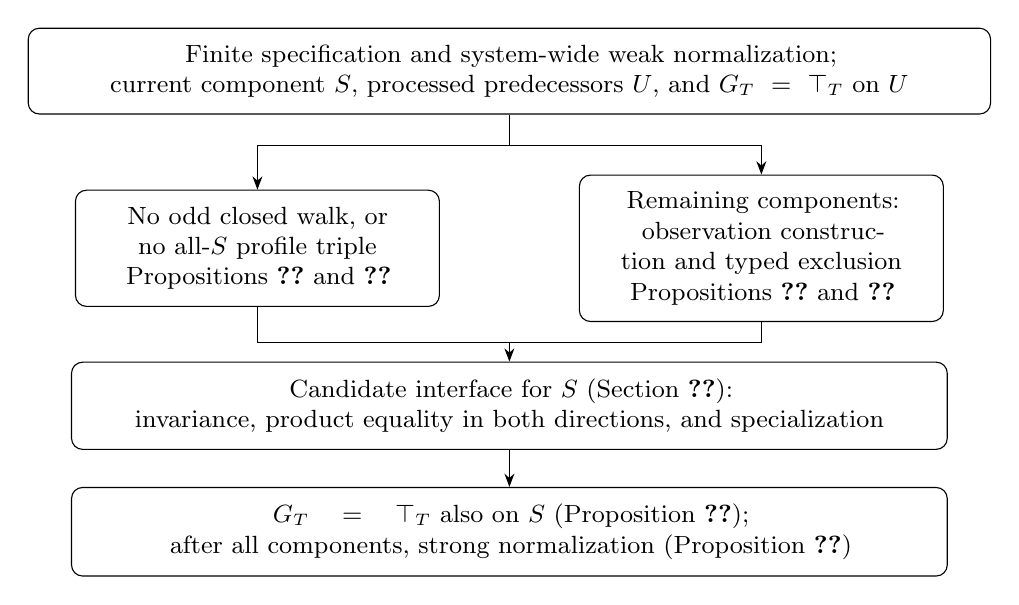
\begin{tikzpicture}[>=Stealth,
  contract/.style={draw,rounded corners,align=center,font=\small,
                   inner sep=6pt,text width=4.2cm}]
\node[contract,text width=11.8cm] (input) at (0,0)
  {Finite specification and system-wide weak normalization;\\
   current component $S$, processed predecessors $U$, and $G_T=\top_T$ on $U$};
\node[contract] (simple) at (-3.2,-2.25)
  {No odd closed walk, or no all-$S$ profile triple\\
   Propositions~\ref{prop:signed-component} and~\ref{prop:one-child-component}};
\node[contract] (remaining) at (3.2,-2.25)
  {Remaining components: observation construction and typed exclusion\\
   Propositions~\ref{obs:interface-theorem} and~\ref{prop:enc-exclusion}};
\node[contract,text width=10.7cm] (interface) at (0,-4.25)
  {Candidate interface for $S$ (Section~\ref{subsec:candidate-interface}):\\
   invariance, product equality in both directions, and specialization};
\node[contract,text width=10.7cm] (advance) at (0,-5.85)
  {$G_T=\top_T$ also on $S$ (Proposition~\ref{prop:advance-component});\\
   after all components, strong normalization (Proposition~\ref{prop:interfaces-imply-sn})};
\draw (input.south) -- (0,-.95);
\draw[->] (0,-.95) -| (simple.north);
\draw[->] (0,-.95) -| (remaining.north);
\draw (simple.south) -- (-3.2,-3.45) -- (0,-3.45);
\draw (remaining.south) -- (3.2,-3.45) -- (0,-3.45);
\draw[->] (0,-3.45) -- (interface.north);
\draw[->] (interface) -- (advance);
\end{tikzpicture}
\caption{The contracts of one component step. The right branch combines
the conditional observation construction with the independent proof of
its graph hypothesis. The arrows to the interface assert the complete
three-part contract, before any use of component advancement.}
\label{fig:component-contracts}
\end{figure}
\FloatBarrier

\section{Two component constructions}
\label{sec:simple-components}

Keep a current component $S$ and the invariant on its processed
predecessors $U$. The first construction uses signs to compensate for
the opposite variances of domain and codomain. The second uses a
single chain in each normal type when its two product children cannot
both remain in $S$.

\subsection{Components without an odd closed walk}

\begin{proposition}[The signed fixed-point construction]
\label{prop:signed-component}
If $S$ has no odd closed walk, it admits the candidate interface.
\end{proposition}

\begin{proof}
Choose a vertex of $S$. Assign to each vertex the parity of any path
from the chosen vertex to it. This is well defined: append a return
path to two proposed paths; different parities would produce an odd
closed walk. Give even vertices sign $+$ and odd vertices sign $-$.
Every internal positive edge preserves sign, and every internal
negative edge reverses sign.

Let $\mathcal T_S$ be the set of actual types with profile in $S$.
It is a set, since these are finite syntax over the countable context
$\Omega$. On
\[
                      \mathcal L=
                  \prod_{T\in\mathcal T_S}\mathcal C(T)
\]
use inclusion in coordinates with sign $+$ and reverse inclusion in
coordinates with sign $-$. This is a complete lattice by
Lemma~\ref{lem:candidate-lattice}. Extend a vector $v$ to actual
types in $U$ by $v_T=\top_T$.

Define an operator $F:\mathcal L\to\mathcal L$. At a nonproduct
type set $F(v)_T=\top_T$. At $T=\Pi x:D.E$, let
\[
 F(v)_T=\{h\in\top_T:\text{for every }n\in v_D,
                                      \ h n\in v_{(E[x:=n])^\#}\}.
\]
All indices belong to $U\cup S$ by the dependency graph, and this
is a candidate by Lemma~\ref{lem:candidate-lattice}.

The operator is monotone in the mixed order. In the usual inclusion
order its product clause is antitone in the domain coordinate and
monotone in every instantiated-codomain coordinate. An internal domain
has the opposite sign to $T$ by its negative edge. An instantiated
codomain in $S$ has the same sign as $T$ by its positive path through
the open codomain: the intermediate vertex must also lie in $S$,
since a vertex in $U$ has all its predecessors in $U$. Coordinates
in $U$ are constant. These observations
give exactly the required coordinatewise monotonicity, in either sign
of the output.

Tarski's fixed-point theorem \cite[Theorem~1]{Tarski1955} gives a fixed
point. We recall its short existence proof, which needs no continuity
assumption. Let $a$ be the supremum of all
$v$ satisfying $v\le F(v)$. For every such $v$, monotonicity gives
$v\le F(v)\le F(a)$, so $a\le F(a)$. Then
$F(a)\le F(F(a))$, making $F(a)$ one of the elements whose supremum
is $a$; hence $F(a)\le a$. Fix such a vector $a$.

No auxiliary parameters are needed. For a generic normal type $T$
with profile in $S$, define $R_T=a_{(T\xi)^\#}$ if its actual
profile is in $S$, and top otherwise. At a generic product with
actual profile in $S$, its actual normalized domain and all actual
instantiated codomains are exactly the indices in the operator clause.
Thus the fixed-point equality gives the required product equality,
with the unique parameter extension.

The actual normalized type determines the candidate, so thinning,
context conversion and pointwise convertible images preserve it.
For specialization the two actual type expressions
\[
 E(\xi[x\mapsto N\xi])
       \quad\hbox{and}\quad ((E[x:=N])^\#)\xi
\]
are convertible by substitution composition and normalization.
Their normal forms are identical. The two candidates are consequently
equal when that profile is in $S$, and both are top in $U$. A generic
child in $U$ remains there under substitution, so no additional case
arises. This proves all interface requirements.
\end{proof}

\subsection{Components with at most one internal product child}

Suppose now that there is no profile triple $(I,J,K)$ with
$I,J,K\in S$. For a normal type $T$ of profile in $S$, start at its
root. At a product continue to its child of profile in $S$, if it has
one; there is at most one. Stop at a nonproduct or at a product with
no such child. This is a finite path in the syntax tree.

If the path ends at a neutral expression whose head $y$ is free in
the starting context of $T$, define the \emph{support} of $T$ to be
$y$. Define its \emph{polarity} to be $+$ or $-$ according to whether
the path takes an even or odd number of domain steps. In every other
case the support is empty. Also declare support empty at a generic
profile outside $S$. In particular a head bound strictly inside
$T$ is not its support. The support of a codomain, considered in its
own extended context, may of course be its immediately preceding
binder.

Assign each declaration of a generic context a bit $0$ or $1$;
these are the parameters $\theta$. At a neutral we use the candidate
extremum selected by its head's bit, with $0$ selecting bottom and $1$
selecting top. Define candidates recursively on normal generic types
as follows. At an actual profile in $U$ use top. At a generic profile
outside $S$ also use top, as in the interface. Otherwise:
\begin{itemize}
\item at a sort use top;
\item at a neutral with head $y$ use
      $\bot_{(T\xi)^\#}$ or $\top_{(T\xi)^\#}$ according to
      $\theta(y)$;
\item at a product $T=\Pi x:D.E$ use the product-test candidate
      in Section~\ref{subsec:candidate-interface}. There is one prescribed
      bit for $x$: use $0$ if the support of $E$ is $x$ with positive
      polarity, $1$ if it is $x$ with negative polarity, and $1$ if
      $x$ is not supported. If $E$ has profile in $U$, its bit is
      irrelevant and we again choose $1$.
\end{itemize}
Every recursive child is smaller syntax; candidate existence follows
from Lemma~\ref{lem:candidate-lattice}. Context variables can always
be assigned bits, and the prescribed extension is nonempty.

\begin{lemma}[Dependence on support]
\label{lem:support-dependence}
For fixed typed actual images, the candidate of an $S$ type depends
on the bits of its starting context only through its support, if any.
Valid thinning and context conversion preserve the support, its
polarity, and the candidates. Pointwise convertible actual images
preserve the candidates when old bits agree.
\end{lemma}

\begin{proof}
Induct on the normal type. Sorts and actual-$U$ cases do not use
bits. A neutral uses only its head bit. At a product, any child in
$U$ is interpreted as top; only the unique $S$ child can depend on
old bits. Its support is propagated to the parent unless it is the
product's own binder, whose bit is fixed by the displayed rule.
This proves the dependence assertion. Profile invariance preserves
the same product path and its domain parity under thinning and
context conversion. In those operations and under convertible images,
the actual normal types agree. The recursive product tests then have
identical domains, codomains and prescribed bits, proving the stated
invariances.
\end{proof}

Use the notation $A\preceq_+B$ for $A\subseteq B$ and
$A\preceq_-B$ for $A\supseteq B$. Regard signs as $+1$ and $-1$
when multiplying them.

\begin{lemma}[Comparison after generic substitution]
\label{lem:support-substitution}
Let $\Gamma,y:B,\Delta$ be valid, let $\Gamma\vdash N:B$, and
let $T$ be a normal type of profile in $S$ in that context. Put
\[
 \Gamma'=\Gamma,\Delta[y:=N],\qquad
                         T'=(T[y:=N])^\#.
\]
Take typed substitutions of the two contexts into $\Omega$ whose
images are compatible with composition: the pre-substitution image
of $y$ is convertible to the actual image of $N$, and the other
images agree up to conversion. Equip the substitutions with bits
$\theta,\theta'$. Fix a comparison sign $\delta\in\{+,-\}$ and
assume:
\begin{enumerate}
\item the bits agree on any variable supported by both $T$ and $T'$;
\item if $y$ supports $T$ with polarity $\varepsilon$, then its
      pre-substitution bit is $0$ when $\delta\varepsilon=+$ and
      $1$ when $\delta\varepsilon=-$.
\end{enumerate}
Then, at their common actual normal type,
\[
             R_T(\xi,\theta)
                  \preceq_\delta R_{T'}(\xi',\theta').
\]
\end{lemma}

\begin{proof}
Induct on the pre-substitution syntax of $T$. The actual normal
types agree by substitution composition and confluence. If their
profile lies in $U$, both candidates are top. Otherwise that profile
lies in $S$, and so does the generic profile of $T'$: profile growth
puts it in $U\cup S$, and a generic profile in $U$ could only have
actual profile in $U$.

A sort is unchanged. A neutral whose head is not $y$ remains a
neutral with the same head after substitution and normalization; if
its actual profile is in $S$, the supported head is common and its
bit agrees. At a neutral headed by $y$, its polarity is positive and
the prescribed bit chooses the least candidate for forward inclusion,
or the greatest candidate for reverse inclusion. This compares it
with every possible candidate of $T'$. In particular we do not
recurse into the possibly larger normal expression obtained by
substituting for $y$.

Let $T=\Pi x:D.E$, choosing $x$ fresh for $N$ and for the
substitution data. The post-substitution type is again a product,
with its two substituted components normalized. Context-convert the
open codomain to the normalized post domain. To compare the product
test candidates in direction $\delta$, compare their domain
candidates in direction $-\delta$. On each common test compare their
codomain candidates in direction $\delta$, extending the actual
images by that same raw test and using the respective prescribed
bits for $x$. For example, for forward inclusion every post domain
test must be a pre domain test, and its pre codomain candidate must
be contained in its post codomain candidate.

If a pre child is in $U$, its generic substitute remains in $U$ and
both actual child candidates are top. If its generic substitute
grows into $U$, the common actual child profile is again in $U$,
with the same conclusion. In all other required child comparisons,
both generic child profiles are in $S$. Such a post child must be
the same unique $S$ child as before substitution: a pre off-path
child in $U$ cannot grow into $S$. Every common supported variable
other than the new binder $x$ therefore inherits the agreement
condition from the parent. If $y$ supports the child, the prescribed
extremum condition is also inherited: a domain step reverses both
the comparison direction and the support polarity, and a codomain
step reverses neither.

It remains to check the bits of $x$ when it is supported in both
open codomains. The pre support path ends at a neutral with head
$x$, which substitution for $y$ cannot change. Every product on
that path persists. The post support path must follow the same
positions: a pre off-path child remains in $U$, while truncation
of the path into $U$ would prevent the post codomain from being
supported by $x$. Thus both paths have the same number of domain
steps, their polarities agree, and the prescribed bits of $x$
agree. If substitution exposes $x$ through a neutral headed by
$y$, that portion of the induction instead stops at the extremum
case already proved; it imposes no further shared-support condition.

All hypotheses of the child inductions now hold. Their inclusions
give the desired product inclusion by the universal test definition,
in either direction. This completes the induction.
\end{proof}

\begin{proposition}[The one-child construction]
\label{prop:one-child-component}
If no profile triple has all three vertices in $S$, then the
bit-parametrized candidates above implement the candidate interface.
\end{proposition}

\begin{proof}
Candidate existence and product equality follow from the recursion.
Lemma~\ref{lem:support-dependence} gives the required invariances.
To verify specialization, let
$T=\Pi x:D.E$, take $\Gamma\vdash N:D$ with $N\xi\in R_D$,
and let $h\in R_T$. Its product test gives
\[
 h(N\xi)\in R_E(\xi[x\mapsto N\xi],\theta_x)
\]
when the actual codomain profile lies in $S$; here $\theta_x$ is
the prescribed binder extension. Apply
Lemma~\ref{lem:support-substitution} to substitution for $x$ in
$E$, with comparison direction $+$. All old bits agree. The
prescribed bit of $x$ is exactly $0$ for positive support and $1$
for negative support, as that lemma requires. It follows that the
last candidate is contained in
$R_{(E[x:=N])^\#}(\xi,\theta)$, proving specialization. At an
actual codomain profile in $U$, the strong-normalization test gives
specialization directly. Arbitrary bits are allowed on the starting
context, and every prescribed or arbitrary binder extension exists.
All interface requirements are satisfied.
\end{proof}

Consequently, only components having both an odd closed walk and a
profile triple entirely inside the component remain. The next
construction will provide their interface under a stated graph
exclusion. Once that exclusion is proved from system-wide weak
normalization, Proposition~\ref{prop:interfaces-imply-sn} completes
the normalization argument.

\section{Observation spaces and substitution-stable candidates}
\label{obs:section}

We now construct the candidate interpretation for the remaining primary
component.  Throughout this section, $S$ is the current component of the
primary graph and $U$ is its predecessor-closed processed part.  We retain
the hypothesis of weak normalization for every legal expression.  We use
the preceding profile and candidate lemmas, including
$G_T=\operatorname{Ty}(T)\cap\mathrm{SN}_\beta$ when $\pi(T)\in U$.
The new input will be the exclusion of a particular finite graph
configuration, stated below and proved in the next part of the argument.
No strong-normalization hypothesis is imposed on substitutions in this
section.

The interpretation of a neutral type must account for substitutions
that replace its head by a product.  We therefore give variables parameters
that record candidates, and interpret the syntax of a substituted term
to determine which candidate to read.  At a function type
$T=\Pi x:D.E$, such a parameter records a base observation.  The
construction supplies spaces only at selected types; whenever the
instantiated result $(E[q/x])^\#$ has a space, a normal argument
$q:D$, together with a parameter for $q$ when its type requires one,
selects a next value in that result space.  The function's space can
therefore depend on the spaces for both its arguments and its results.  These dependencies
can cycle, so ordinary recursion on the displayed type does not suffice.

The graph below identifies which spaces are needed and separates two
ways to construct them.  Some admit a description by finite observation
paths or a decreasing count of type nodes.  For the others we build two
spaces together: unrestricted tables on one side and tables with a
uniform finite bound on their payload dependence on the other.  After
constructing the spaces, we prove that every finite typed syntax tree
can be evaluated in them.  Substitution and reduction require an
additional condition, called goodness, which holds for the normal
syntax used to define our candidates.  That final transport result will
supply the specialization property of
the candidate interface.

\subsection{Which values require observations?}
\label{obs:graphs}

There are two different profiles to keep apart.  A neutral type sorted
at $s$ has expression profile $\{s\}$; a value interpreting that type
is indexed by its expected type $s$, whose profile is
$\operatorname{Ax}(s)$.  These axiom profiles are the starting points
for deciding which parameter spaces are needed.  The remaining graph
definitions follow the dependencies of those spaces toward
domains that are tested by products within $S$.

Let $H$ be the closure under primary positive paths of
\[
 \{\operatorname{Ax}(s):\{s\}\in S,
                         \ \operatorname{Ax}(s)\ne\varnothing\}.
\]
The \emph{secondary graph} has vertex set $H$.  It retains all primary
positive edges between these vertices.  It retains the negative edge
$I\longrightarrow K$ belonging to a profile triple $(I,J,K)$ precisely
when $I,J,K\in H$.  A vertex $I\in H$ is \emph{direct} if some profile
triple $(I,J,K)$ has $J,K\in S$; here $J,K$ need not belong to $H$.
A vertex is \emph{active} if it has a secondary path to a direct vertex.
Only the induced graph on active vertices will be used below.

An active vertex is \emph{plain} if paths from it to direct vertices
occur with both parities.  Otherwise it is \emph{free}; its sign is $+$
if those paths are even and $-$ if they are odd.  A path of length zero
is even, so a free direct vertex has sign $+$.

This last observation will control the later uniform bounds.  A product
test whose product and instantiated codomain profiles remain in $S$
has its open codomain profile in $S$ as well, by their positive ascent.
A domain profile that is active is therefore direct.  Such a test may
quantify over parameters at plain or free plus profiles, but never at
free minus profiles.
This fact will let one finite dependence bound survive all the parameter
choices in a product test.

\begin{lemma}[Signs and dependencies]\label{obs:graph-lemma}
An active predecessor of a plain vertex is plain.  Along an edge between
free vertices, the sign is preserved on a positive edge and reversed on
a negative edge.

Let $T=\Pi x:D.E$ be a normalized actual type, put
$I=\pi(D)$, $J=\pi(E)$, and $K=\pi(T)$, and let
$q\in\operatorname{Ty}(D)$.  Put $T_q=(E[q/x])^\#$ and $L=\pi(T_q)$.
If $K,L$ are active, then $J$ is active, and $I$ is active whenever
$I\in H$.  If instead $K,L\in S$, then $J\in S$ and every active $I$
is direct.
\end{lemma}
\begin{proof}
Prepending the edge in question to paths to a direct vertex proves the
sign statements.  Profile growth and the product edge give the positive
path
\[
                         L\longrightarrow J\longrightarrow K,
\]
where the first edge is omitted when $L=J$.  Since $L\in H$ and $H$ is
positive-path closed, $J\in H$.  Its path to the active vertex $K$ makes
$J$ active.  If $I\in H$, the negative edge of $(I,J,K)$ is retained,
so $I$ is active too.  When $K,L\in S$, the displayed path cannot leave
their primary strongly connected component.  Thus $J\in S$, and the
definition of direct applies.
\end{proof}

The \emph{layer} of a type $T$ is $\pi(T)$.  A type is active, plain, or
free of a given sign when its layer is so; an empty layer is inactive.
These terms concern the type of a value, not the profile of the value
itself.

Here is the promised graph hypothesis.
\begin{equation}\label{obs:forbidden}
\begin{gathered}
\text{There is no plain active secondary strongly connected component $C$}\\[-2pt]
\text{with an internal negative edge, a profile triple $(I,J,K)$ with $J,K\in C$,}\\[-2pt]
\text{and a sort $s$ such that $\{s\}\in C$, $\operatorname{Ax}(s)\ne\varnothing$, and}\\[-2pt]
                  \operatorname{Ax}(s)\longrightarrow I
                  \text{ by a primary positive path.}
\end{gathered}
\end{equation}
All results in this section are conditional on
\eqref{obs:forbidden}.  The later typed contradiction will derive this
condition from the same system-wide weak-normalization hypothesis.

\subsection{Actual frames and plain observation spaces}
\label{obs:plain-spaces}

Let $\mathcal B$ be the set of assignments choosing one candidate at
every actual type.  Its distinguished member $\mathbf t$ chooses every
top candidate.  All types and expressions here are syntax over finite
prefixes of $\Omega$, modulo $\alpha$-equivalence, so their collections
and $\mathcal B$ are sets.

We construct a nonempty set $\mathcal K_T$ of parameters for every
active actual type $T$.  For a plain type we require the following
precise prefix description.  If $T=\Pi x:D.E$, a \emph{legal frame at
$T$} consists of a normal term $q\in\operatorname{Ty}(D)$ for which
$T_q=(E[q/x])^\#$ is active, together with a parameter
$v\in\mathcal K_D$ if $D$ is active.  If $D$ is inactive there is one
absent-payload symbol in place of $v$.  Its target is $T_q$.  A
nonproduct type has no legal frames.  Write $\mathcal F_T$ for this
set of frames.  The desired description is the bijection
\begin{equation}\label{obs:plain-prefix}
 \mathcal K_T\ \simeq\
 \mathcal B\times
       \prod_{a\in\mathcal F_T}\mathcal K_{\operatorname{target}(a)}.
\end{equation}
We call its first coordinate the base and its $a$-coordinate the next
value.  By Lemma~\ref{obs:graph-lemma}, all active spaces occurring on
the right are plain when $T$ is plain, and their secondary components
precede or equal that of $T$.

\begin{lemma}[Construction of plain spaces]\label{obs:plain-construction}
Under \eqref{obs:forbidden}, the plain spaces admit
\eqref{obs:plain-prefix}.  They also admit distinguished values whose
bases are $\mathbf t$ and whose next values are distinguished values.
\end{lemma}
\begin{proof}
Process the finitely many plain secondary components in source order.
Suppose first that a component $C$ has no internal negative edge.
Every active domain used by a legal frame at a type of layer in $C$
then lies in an earlier component: otherwise the frame's triple, whose
open codomain is active, would contribute an internal negative edge.
Thus all frame alphabets can be specified without using a space whose
layer belongs to $C$.

For $\pi(T)\in C$, consider finite paths of legal frames beginning at
$T$.  A continuing path has all its target layers in $C$, and includes
the empty path.  An exiting path has all but its final target layer in
$C$ and its final target in an earlier component.  Define $\mathcal K_T$
to be the set of tables assigning a member of $\mathcal B$ to each
continuing path and a member of the final target space to each exiting
path.  Split a table according to the empty path and the first frame.
For a frame staying in $C$, its suffix table is exactly a table of the
same kind starting at its target.  For an exiting frame its output is
already a value of the target space.  This gives the bijection
\eqref{obs:plain-prefix} in both directions.  The constant top outputs
and previously chosen exit defaults define the distinguished table.

Now let $C$ have an internal negative edge.  For every normalized type
$T$ of layer in $C$, define a positive integer $p_C(T)$ as follows.
Count its root.  At a product with child layers $I,J$, continue into
the codomain when $J\in C$, and into the domain when $I\in C$ and
$J$ is active.  Apply the same rule recursively at counted children,
using the binder context in the codomain.  This counts a subset of a
finite syntax tree.  Profile invariance makes the count independent of
the prefix and unchanged by valid thinning or context conversion.

For a legal frame at $T=\Pi x:D.E$, write
$I=\pi(D)$, $J=\pi(E)$, $K=\pi(T)$, and $L=\pi(T_q)$.
A same-$C$ domain has smaller count.  We claim
that its same-$C$ target also satisfies
\begin{equation}\label{obs:potential-drop}
               p_C(T_q)\le p_C(E)<p_C(T).
\end{equation}
Here $J\in C$ follows from the positive ascent in
Lemma~\ref{obs:graph-lemma}; hence $p_C(E)$ is defined.

To prove the first inequality, thin $T$ and $q$ to a common prefix,
choosing the displayed binder fresh.  Associate to every counted node
of $(E[q/x])^\#$ its position string.  We show that the same position
is a counted node of $E$.  The induction along a position maintains
that the corresponding pre- and post-substitution parent profiles both
lie in $C$; at the root these are $J$ and $L$.  At a pre-substitution
product the post normal form is a product with componentwise substituted
normal forms.  Write $I_0,J_0,K_0$ for its pre domain, codomain, and
parent profiles, and $I_1,J_1,K_1$ for the post profiles.  Profile growth
gives $I_1\supseteq I_0$ and $J_1\supseteq J_0$, also under binders
after context conversion.

If the post codomain is counted, then $J_1\in C$, and the positive
path $J_1\longrightarrow J_0\longrightarrow K_0$ has both endpoints
in $C$.  Hence $J_0\in C$, so the pre codomain is counted too.  If
the post domain is counted, then $I_1\in C$ and $J_1$ is active.
The inclusion paths put $I_0,J_0$ in $H$.  Since $K_0\in C\subseteq H$,
the pre triple has a retained negative edge $I_0\longrightarrow K_0$.
The path
\[
                  I_1\longrightarrow I_0\longrightarrow K_0
\]
again has endpoints in $C$, so $I_0\in C$.  Also the positive edge
$J_0\longrightarrow K_0$ makes $J_0$ active.  Thus the pre domain is
counted.  In either case the pre- and post-substitution profiles of the
selected child lie in $C$, which preserves the induction invariant for
the next position.  Inclusion edges in these paths are omitted when
the profiles are equal.

The association could fail only if a pre neutral leaf became a product.
Sorts are unchanged, and a neutral with any other head remains neutral
after substitution and normalization.  Its head must therefore be the
substituted variable $x$.  Let its singleton profile be $\{s\}$;
this lies in $C$.  The sort $s$ is sorted, so
$\operatorname{Ax}(s)\ne\varnothing$.  Trace the original $x$-headed
spine backward through its normalized successive typing products.
At each application the result layer has a primary positive path to
the function layer.  Starting with the layer
$\operatorname{Ax}(s)$ of its type $s$, concatenate these paths to
obtain a positive path to $\pi(D)=I$.  The outer product has
$J,K\in C$.  This is forbidden by \eqref{obs:forbidden}.  No leaf
therefore expands.  Position strings give the required injection of
counted nodes and prove \eqref{obs:potential-drop}.

Define \eqref{obs:plain-prefix} by induction on $p_C(T)$, simultaneously
for all types with the same count.  Every same-component space on its
right is already constructed by the strict inequalities just proved;
all other spaces come from earlier components.  The product of the
specified nonempty sets is nonempty, with the explicit element whose
base is $\mathbf t$ and whose next values are the already specified
defaults.  This completes the construction.
\end{proof}

\subsection{Free observation spaces}
\label{obs:free-spaces}

The construction in this subsection is purely set-theoretic.  The typing
conditions on frames will be imposed by evaluation; they do not restrict
the tables constructed here.  Fix the set $\mathcal Q$ of normal syntax
over $\Omega$, with bound names identified up to $\alpha$-conversion.
Let $\mathcal T_{\mathrm{pl}}$ be the set of actual plain active types,
and suppose that the nonempty spaces $\mathcal K_D$ have already been
constructed for $D\in\mathcal T_{\mathrm{pl}}$.  The fixed set of tagged
plain values is
\begin{equation}
  \mathcal V_{\mathrm{pl}}
   =\coprod_{D\in\mathcal T_{\mathrm{pl}}}
       \bigl(\{D\}\times\mathcal K_D\bigr).
  \label{obs:free-plain-values}
\end{equation}
Thus a member of $\mathcal V_{\mathrm{pl}}$ remembers both its type $D$ and its value
$v\in\mathcal K_D$.  Let $\mathcal B$ be the set of base observations:
a member chooses a candidate at every actual type.  Write
$\mathbf t\in\mathcal B$ for the choice of the top candidate everywhere.
For the present construction only the set $\mathcal B$ and its
distinguished member $\mathbf t$ are needed.  Put
\[
  \mathcal O=\{\star\}\sqcup\mathcal V_{\mathrm{pl}},
\]
where the union is disjoint.  In particular, both output sets
$\mathcal B$ and $\mathcal O$ have specified default elements, even if
there are no plain active types.

\paragraph{Frames, stacks, and tables.}
For any set $Y$ define the payload set
\[
  V(Y)
   =\{\mathrm{none}\}
      \sqcup\bigl(\{\mathrm{opp}\}\times Y\bigr)
      \sqcup\bigl(\{\mathrm{plain}\}\times\mathcal V_{\mathrm{pl}}\bigr).
\]
The three tags make these alternatives disjoint.  Define continue and
exit frames by
\[
  F_c(Y)=\mathcal Q\times V(Y)\times\{c\},
  \qquad
  F_e(Y)=\mathcal Q\times V(Y)\times\{e\}.
\]
Here $Y$ is the space of opposite-sign payloads.  The set of non-exiting
stacks and the set of exiting stacks are, respectively,
\begin{equation}
  S_c(Y)=\coprod_{n\geq 0} F_c(Y)^n,
  \qquad
  S_e(Y)=\coprod_{n\geq 0}
                 \bigl(F_c(Y)^n\times F_e(Y)\bigr).
  \label{obs:free-stacks}
\end{equation}
Thus $S_c(Y)$ contains the empty stack $\epsilon$, and an exit frame
occurs exactly once, at the end of a stack in $S_e(Y)$.  Set
\begin{equation}
  \operatorname{Tab}(Y)
      =\mathcal B^{S_c(Y)}\times\mathcal O^{S_e(Y)}.
  \label{obs:free-tab}
\end{equation}
A table $t=(t_c,t_e)$ gives a base observation on each non-exiting
stack and an exit observation on each exiting stack.  Its default
$d_Y$ is specified by
\[
  (d_Y)_c(\sigma)=\mathbf t,
  \qquad
  (d_Y)_e(\tau)=\star.
\]
Consequently $\operatorname{Tab}(Y)$ is nonempty for every $Y$,
including $Y=\emptyset$.

We seek two spaces whose tables take values of the opposite sign as
payloads.  Their construction must solve two different problems.  A plus
value should accept every finite stack of minus values.  A minus value
must be representable at a finite stage, even though it is tested on
arbitrarily many plus values and arbitrarily long stacks.  Choosing a
stage separately for each stack would not give that representation.

The construction below supplies a space $C_*$ of minus values and the
full space $P_*=\operatorname{Tab}(C_*)$ of plus tables.  Increasing
stages $C_r$ give restrictions
$\rho_r:P_*\to P_r=\operatorname{Tab}(C_r)$ of plus tables.
A table on plus payloads represents a minus value precisely when
one index $r$ works for every observation: replacing each plus payload
$p$ by $p'$ with $\rho_r(p)=\rho_r(p')$ leaves the table output
unchanged.  Finally, fixing any continue prefix must again give a value
of the same sign; on the minus side it must retain the same representing
stage.  These are the representation and slicing properties that typed
evaluation will use.  We first construct the stages and then prove this
characterization.

\paragraph{Relabeling and contravariance.}
A map $f:Y\to Z$ induces stack maps
$S_a(f):S_a(Y)\to S_a(Z)$ for $a\in\{c,e\}$.
These replace $(\mathrm{opp},y)$ by $(\mathrm{opp},f(y))$ in each
payload position.  Keys, flags, and the other payload alternatives
are unchanged.  Define
\begin{equation}
  \operatorname{Tab}(f):\operatorname{Tab}(Z)
                  \longrightarrow\operatorname{Tab}(Y),
  \qquad
  \bigl(\operatorname{Tab}(f)(t)\bigr)_a
                   =t_a\circ S_a(f).
  \label{obs:free-contravariance}
\end{equation}
Relabeling preserves identities and composition.  Hence
\[
  \operatorname{Tab}(\operatorname{id}_Y)
     =\operatorname{id}_{\operatorname{Tab}(Y)},
  \qquad
  \operatorname{Tab}(g\circ f)
     =\operatorname{Tab}(f)\circ\operatorname{Tab}(g).
\]
It also preserves the default tables:
$\operatorname{Tab}(f)(d_Z)=d_Y$.

We will use the following two elementary facts.
\begin{enumerate}
\item If $f$ is injective, then $S_c(f)$ and $S_e(f)$ are injective,
and $\operatorname{Tab}(f)$ is surjective.  Indeed, given a table on
$Y$, define a table on $Z$ by transporting its values to the images
of $S_c(f)$ and $S_e(f)$, and assigning $\mathbf t$ or $\star$ on the
respective complements.  Injectivity makes the transported values
unambiguous, and restriction recovers the given table.
\item If $f$ is surjective, then $S_c(f)$ and $S_e(f)$ are surjective,
and $\operatorname{Tab}(f)$ is injective.  To lift a stack, lift its
finitely many opposite payloads through $f$.  If two tables become
equal after precomposition with these surjective stack maps, they
agree on every stack and therefore are equal.
\end{enumerate}
In particular these statements apply when an opposite payload set is
empty; the stacks without opposite payloads remain available.

\paragraph{The alternating chain.}
Define, for $r=0,1,2,\ldots$,
\begin{equation}
  C_0=\emptyset,
  \qquad P_r=\operatorname{Tab}(C_r),
  \qquad C_{r+1}=\operatorname{Tab}(P_r).
  \label{obs:free-stages}
\end{equation}
Let $i_0:C_0\to C_1$ be the empty map.  Inductively, once
$i_r:C_r\to C_{r+1}$ is defined, put
\begin{equation}
  j_r=\operatorname{Tab}(i_r):P_{r+1}\longrightarrow P_r,
  \qquad
  i_{r+1}=\operatorname{Tab}(j_r):C_{r+1}\longrightarrow C_{r+2}.
  \label{obs:free-bonding}
\end{equation}
The preceding facts prove by induction that every $i_r$ is injective
and every $j_r$ is surjective.  Each $j_r$ is restriction to stacks
whose opposite payloads lie in the embedded copy of $C_r$; its
surjectivity has the explicit default-extension proof above.

For $r\leq s$, write $i_{r,s}:C_r\to C_s$ for the composite of the
injections, with $i_{r,r}$ the identity.  Let $C_*$ be the set colimit
of this chain.  Explicitly, take the disjoint union of the $C_r$ and
identify $(r,x)$ with $(s,y)$ precisely when, at some common stage
$m\geq r,s$,
\[
  i_{r,m}(x)=i_{s,m}(y).
\]
The canonical maps $e_r:C_r\to C_*$ are injective and satisfy
$e_{r+1}\circ i_r=e_r$.  Their images form an increasing union
equal to $C_*$.  We may therefore regard the stages as nested
subsets after these identifications.  Every finite family of elements
of $C_*$ lies in a common stage: choose a representing stage for
each element and then take their maximum.  Every element in fact
has a representative in some $C_{r+1}$, since $C_0$ is empty.

\paragraph{Final plus tables and finite-stage agreement.}
Put
\begin{equation}
  P_*=\operatorname{Tab}(C_*),
  \qquad
  \rho_r=\operatorname{Tab}(e_r):P_*\longrightarrow P_r.
  \label{obs:free-final-plus}
\end{equation}
Each $\rho_r$ is surjective, by default extension along the injection
$e_r$.  Contravariance and the identities for $e_r$ give
\begin{equation}
  \rho_r=j_r\circ\rho_{r+1}.
  \label{obs:free-restriction-compatibility}
\end{equation}
For $p,p'\in P_*$ write
\begin{equation}
  p\equiv_r p' \quad\Longleftrightarrow\quad
           \rho_r(p)=\rho_r(p').
  \label{obs:free-equivalence}
\end{equation}
Agreement at a larger stage implies agreement at every smaller
stage, by repeated use of
\eqref{obs:free-restriction-compatibility}.

Every stack in $S_a(C_*)$, for $a\in\{c,e\}$, belongs to the image
of $S_a(e_r)$ for some $r$: it has only finitely many opposite
payloads, which lie in a common stage.  The same holds for any
finite family of stacks, with one common $r$.  It follows that
\begin{equation}
  \bigl(p\equiv_r p'\text{ for every }r\bigr)
       \quad\Longleftrightarrow\quad p=p'.
  \label{obs:free-separation}
\end{equation}
For the forward implication, lift any specified final stack from a
common stage and evaluate the equality $\rho_r(p)=\rho_r(p')$ on
that lift.  The reverse implication is immediate.  No assertion
that a plus table itself belongs to a finite stage is needed.

\paragraph{Final minus behaviors.}
For each $r\geq0$, define
\begin{equation}
  \beta_r=\operatorname{Tab}(\rho_r):
        C_{r+1}=\operatorname{Tab}(P_r)
            \longrightarrow\operatorname{Tab}(P_*).
  \label{obs:free-behavior-stage}
\end{equation}
In coordinates, for $u\in C_{r+1}$ and $\sigma\in S_a(P_*)$,
\[
  \bigl(\beta_r(u)\bigr)_a(\sigma)
       =u_a\bigl(S_a(\rho_r)(\sigma)\bigr).
\]
Thus each plus payload of a final stack is first restricted to
$P_r$.  Since $\rho_r$ is surjective, $\beta_r$ is injective.
Moreover,
\begin{align*}
  \beta_{r+1}\circ i_{r+1}
    &=\operatorname{Tab}(\rho_{r+1})
                          \circ\operatorname{Tab}(j_r)\\
    &=\operatorname{Tab}(j_r\circ\rho_{r+1})
      =\operatorname{Tab}(\rho_r)=\beta_r.
\end{align*}
These maps consequently induce a well-defined map
\begin{equation}
  \beta:C_*\longrightarrow\operatorname{Tab}(P_*),
  \qquad
  \beta(e_{r+1}(u))=\beta_r(u).
  \label{obs:free-behavior}
\end{equation}
It is injective: represent any two proposed equal-behavior elements
at a common stage $C_{r+1}$ and use the injectivity of $\beta_r$.
We henceforth evaluate a minus value through this behavior map.

The defaults are compatible with all bonding maps.  In particular,
the default elements $d_{P_r}\in C_{r+1}$ represent one element of
$C_*$, whose behavior is $d_{P_*}$.  The plus default is
$d_{C_*}\in P_*$.  Both free spaces are therefore nonempty.

\paragraph{Exact characterization by a uniform stage bound.}
Fix $r$.  For $a\in\{c,e\}$ and $\sigma,\tau\in S_a(P_*)$ write
$\sigma\sim_r\tau$ when they have identical lengths, keys, flags,
and payload alternatives, their plain payloads are identical, and
each corresponding pair of opposite payloads $p,p'$ satisfies
$p\equiv_r p'$.  Equivalently,
\begin{equation}
  \sigma\sim_r\tau
    \quad\Longleftrightarrow\quad
  S_a(\rho_r)(\sigma)=S_a(\rho_r)(\tau).
  \label{obs:free-stack-equivalence}
\end{equation}
This equivalence follows directly from the disjoint payload tags
and the definition of stack relabeling.

For a final table $t\in\operatorname{Tab}(P_*)$, the following
conditions are equivalent:
\begin{enumerate}
\item $t$ belongs to the image of $\beta_r$.
\item For both $a=c$ and $a=e$, the equality
      $\sigma\sim_r\tau$ implies $t_a(\sigma)=t_a(\tau)$.
\end{enumerate}
The first condition implies the second by
\eqref{obs:free-behavior-stage}.  Conversely, each
$S_a(\rho_r)$ is surjective, since a finite stack of elements of
$P_r$ can be lifted through the surjection $\rho_r$.  For
$\eta\in S_a(P_r)$ define $u_a(\eta)$ to be $t_a(\sigma)$ for
any lift $\sigma$ of $\eta$.  Such a lift exists, and any two lifts
are $\sim_r$-equivalent by
\eqref{obs:free-stack-equivalence}.  The second condition therefore
makes the definition unambiguous.  It defines a unique
$u\in\operatorname{Tab}(P_r)=C_{r+1}$ with $\beta_r(u)=t$.
This proves the equivalence and uniqueness of the factor.

Consequently
\begin{equation}
  \beta(C_*)
    =\bigcup_{r\geq0}\beta_r(C_{r+1})
    =\left\{
       t\in\operatorname{Tab}(P_*):
       \begin{array}{l}
       \text{for some }r,\text{ each }t_a\text{ is constant}\\
       \text{on every }\sim_r\text{-class},\quad a\in\{c,e\}
       \end{array}
       \right\}.
  \label{obs:free-uniform-factorization}
\end{equation}
The one stage $r$ here is uniform over all stack lengths, keys,
payloads, and both kinds of ending.  The preceding argument proves
factorization for precisely this uniform condition.

\paragraph{Continue-prefix slicing.}
If $\sigma\in S_c(Y)$ and $t\in\operatorname{Tab}(Y)$, define
the slice $t|\sigma\in\operatorname{Tab}(Y)$ by
\begin{equation}
  (t|\sigma)_a(\tau)=t_a(\sigma\tau),
       \qquad \tau\in S_a(Y),\quad a\in\{c,e\},
  \label{obs:free-slice}
\end{equation}
where juxtaposition denotes concatenation.  The prefix has only
continue frames, so concatenation preserves the kind of ending.
This immediately gives slices of plus tables, by taking $Y=C_*$.

For minus tables, slicing preserves the representing stage.
For $u\in C_{r+1}$ and $\sigma\in S_c(P_*)$,
stack relabeling commutes with concatenation and gives
\begin{equation}
  \beta_r(u)|\sigma
     =\beta_r\bigl(u|S_c(\rho_r)(\sigma)\bigr).
  \label{obs:free-slice-bound}
\end{equation}
To check this equality, evaluate either side on
$\tau\in S_a(P_*)$; both values are
\[
  u_a\bigl(S_c(\rho_r)(\sigma)\,
                 S_a(\rho_r)(\tau)\bigr).
\]
The sliced table inside $\beta_r$ belongs to
$\operatorname{Tab}(P_r)=C_{r+1}$.  Thus a minus value represented
at $C_{r+1}$ has every continue-prefix slice represented at that
same stage.  Because $\beta$ is injective, this defines an intrinsic
slice on $C_*$, independent of the chosen representing stage.
Equivalently, fixing a prefix preserves invariance under
$\sim_r$ on all remaining payloads.  Default tables slice to
default tables.  Define
\[
 \mathcal K_T=\begin{cases}P_*,&T\text{ is free plus},\\
 C_*,&T\text{ is free minus}.\end{cases}
\]
Evaluate a minus value through the injective behavior map $\beta$.
Thus a plus value is an arbitrary table, whereas a proposed minus
behavior defines a value only after one uniform stage bound has been
proved.  The evaluation of a lambda at a free minus type will be the
place where this distinction matters.


\subsection{Finite typing trees and environments}
\label{obs:trees}

Evaluation must remember the particular product used to type an
application.  We therefore equip the finite syntax tree of a judgment
$\Gamma\vdash M:T$ with generation data.  At each node we store its
expected-type judgment and a core typing converting to that expectation:
the declaration at a variable; the axiom target at a sort; the two child
sorts and the formation triple at a product; the annotation sort, body
type and supporting product typing at a lambda; and the function's
exact product expectation and the argument's domain expectation at an
application.  We include the annotation's typing at a lambda.  These
data exist by generation; their witnesses are finite.  They do not
require uniqueness of sorts or formation rules.

The following operations on these trees will be used.  Valid thinning
and context conversion transport all judgments and generation witnesses.
At a variable the implicit core declaration is changed accordingly.
Retargeting a root changes its expected type to a convertible type at
which the same expression is typed; it retains the core data and all
children.  Capture-avoiding substitution transports the stored judgments
and grafts copies of the argument tree at occurrences of the substituted
variable, thinning and retargeting those copies as needed.  These
operations use only the previously established metatheory.

An environment for a finite generic context $\Gamma$ is a typed
substitution $\xi:\Gamma\to\Omega$, with arbitrary raw term images,
together with a parameter $\theta_x\in\mathcal K_{(A\xi)^\#}$ for each
declaration $x:A$ whose actual type $(A\xi)^\#$ is active.  Declaration
types are evaluated at their prefixes.  The notation $A\xi$ may also
use the whole substitution, since no later variable is free in $A$.
An extension by $x:=n$ is typed whenever $n$ has the actual normalized
domain type; conversion gives its required raw type.  At an active
domain it may be accompanied by any parameter in the corresponding
space.  At an inactive domain no parameter is supplied.

Two environments are \emph{compatible} if their raw images are
pointwise convertible and their corresponding parameters are equal.
Their actual normalized types are equal, so this equality of parameters
is well-typed.  All prefix changes are understood by thinning.

\subsection{Evaluation and reading candidates}
\label{obs:evaluation}

For a typing tree $t$ of $M:T$ and an environment $(\xi,\theta)$, define
\[
 \operatorname{Val}(t;\xi,\theta)\in\mathcal K_{(T\xi)^\#}
 \quad\text{when $(T\xi)^\#$ is active.}
\]
For a tree of $M:s$ with literal expected sort, define
$\operatorname{Read}(t;\xi,\theta)$ to be a candidate at the actual
expression $(M\xi)^\#$.  The two constructions are distinct: the
space index of the first is the actual \emph{type}; the candidate index
of the second is the actual \emph{expression}.

Every active space has a base in $\mathcal B$: its prefix base when
plain, and its empty-stack output when free.  Write
$\operatorname{base}(v)[A]$ for the candidate at actual type $A$ selected
by that base.

First specify the product candidate used in both constructions.
For a product tree with children $D:a,E:b$, put
\[
 D_0=(D\xi)^\#,
 \qquad A=((\Pi x:D.E)\xi)^\#,
 \qquad A_n=(E\xi[x:=n])^\#.
\]
The binder is chosen fresh for the images.
When $\pi(A)\in S$, define $\mathcal P(t;\xi,\theta)$ to consist of
the strongly normalizing $h\in\operatorname{Ty}(A)$ satisfying the
following test.  The tester $n$ ranges over
\[
 \begin{cases}
 \operatorname{Read}(D:a;\xi,\theta),&\pi(D_0)\in S,\\
 \operatorname{Ty}(D_0)\cap\mathrm{SN}_\beta,&\pi(D_0)\notin S.
 \end{cases}
\]
If $\pi(A_n)\in S$, require
\begin{equation}\label{obs:product-test}
 h\,n\in\operatorname{Read}(E:b;\xi[x:=n],\theta[x:=v])
\end{equation}
for every $v\in\mathcal K_{D_0}$ when $D_0$ is active, and for the
unique parameter-free extension otherwise.  If $\pi(A_n)\notin S$,
require just that $h\,n$ be strongly normalizing at its exact type
$A_n$.  Normalization and conversion identify $A_n$ with the
instantiation of the normalized product $A$.  The candidate test lemma
therefore shows that $\mathcal P$ is a candidate whenever its child
Reads are defined.

The clauses for $\operatorname{Val}$ are as follows.
\begin{enumerate}
\item A variable looks up its parameter.  A sort has the distinguished
      value of its actual type.
\item At a product with literal core sort $s$, start with the
      distinguished value.  If $\{s\}\in S$ and the profile of the
      actual product expression is in $S$, replace its base coordinate
      at that expression by $\mathcal P$.  All other coordinates and
      later observations stay distinguished.
\item At a lambda $\lambda x:D.P$, the base is $\mathbf t$.
      If its actual type is plain, prescribe its next value at every
      legal frame $(q,v)$ to be
      \begin{equation}\label{obs:lambda-equation}
       \operatorname{Val}(P;\xi[x:=q],\theta[x:=v]).
      \end{equation}
      The absent-payload convention applies when the domain is
      inactive.  Product compatibility gives the asserted target type.

      At a free actual type, give the following behavior on raw stacks.
      For a nonempty stack, check that its first key $q$ is a normal
      term at the actual normalized domain and that its next actual
      type is active.  Check its payload: absent at an inactive domain,
      an opposite-sign free value at a free domain, or a plain value
      with exactly the domain's type tag at a plain domain.  Finally
      require a continue flag exactly when the next type is free, and
      an exit flag exactly when it is plain.  Lemma~\ref{obs:graph-lemma}
      gives the same sign at a free next type and the opposite sign at
      a free domain.  On a valid continue frame, observe
      \eqref{obs:lambda-equation} on the remaining stack.  On a valid
      exit frame, return that value tagged with its plain target type.
      On an invalid stack, return the distinguished output for its
      ending.  The finite-bound lemma below proves that this behavior
      represents a member of the minus space when the lambda is minus.
\item At an application $F\,N$ with active actual result type, return
      its distinguished value if the function's actual type is
      inactive.  Otherwise use the frame with key $(N\xi)^\#$ and
      payload $\operatorname{Val}(N)$ when its actual domain is active.
      At a plain function take its next value.  At a free function take
      a continue slice when the result is free.  When the result is
      plain, take the exit output and project its correctly tagged
      value, using the distinguished target value for a missing or
      wrong tag.  The graph lemma and subject reduction make this a
      legal frame with the asserted target.
\end{enumerate}

The clauses for $\operatorname{Read}(M:s)$ are these.  If the actual
expression profile is outside $S$, or if $M$ is a literal sort, use the
top candidate.  At product syntax with actual profile in $S$, use
$\mathcal P$.  At all other syntax with actual profile in $S$, use
\begin{equation}\label{obs:read-base}
 \operatorname{base}(\operatorname{Val}(M:s))[\,(M\xi)^\#\,]
\end{equation}
if $\{s\}\in S$ and $\operatorname{Ax}(s)$ is active; use top otherwise.
The layer required for the Val in \eqref{obs:read-base} is exactly
$\operatorname{Ax}(s)$.

Val calls Read only on strict syntax children.  Read may call Val at
the same root.  Thus the intended recursion order is syntax size,
with Val preceding Read at a fixed size.  The next lemma establishes
totality as well as the only representability issue, at a minus lambda.
It also establishes compatible-image invariance without assuming that
the raw images are strongly normalizing.

\subsection{Uniform finite bounds for typed evaluation}
\label{obs:bound-section}

We verify that the preceding clauses define actual values in the stated
spaces, including at free minus layers.  In this subsection a typing tree
is fixed, but its typed substitution and its parameters may vary.  Bounds
will depend only on the finite tree and an integer, and not on any of
these images or parameters.  We use the images of $C_k$ in $C_*$ without
further notation.

Two environments for the same tree are called \emph{image-compatible} if their
term images are pointwise convertible.  Their actual normalized
declaration types consequently agree.  For $r\geq 0$, say that they
\emph{agree to level $r$} if, in addition, corresponding plain and minus
parameters are equal and corresponding plus parameters are
$\equiv_r$-equivalent.  Parameters at inactive declarations are absent.
An environment is \emph{minus-bounded by $k$} if all its minus parameters
belong to $C_k$.  In particular, being minus-bounded by zero means having
no minus parameters.  Every finite environment is minus-bounded by some
$k$, since $C_*$ is the increasing union of its stages.

\paragraph{The three binder facts.}
\label{obs:bound-binder-facts}
The following consequences of the graph definitions will be used
repeatedly.  Suppose a normalized product has profile $K$, domain profile
$I$, open codomain profile $J$, and instantiated codomain profile $L$.
If $K$ and $L$ are active, the positive ascent $L\longrightarrow
J\longrightarrow K$ makes $J$ active.  If also $I\in H$, the retained
negative edge $I\longrightarrow K$ makes $I$ active.  Therefore:
\begin{enumerate}
\item If $K$ is plain, every active frame payload and every active
continuation is plain: an active edge into a plain vertex starts at a
plain vertex, and the same holds for a positive path into a plain vertex.
\item If $K$ and $L$ are free, they have the same sign; a free domain
payload has the opposite sign to $K$.
\item If $K,L\in S$, then $J\in S$, since $J$ lies on a path between two
vertices of the primary strongly connected component $S$.  Hence an
active $I$ is direct.  A free direct vertex is plus, so such a domain is
never free minus.
\end{enumerate}
The last assertion is the reason that universal quantification over
payloads in a product candidate preserves a fixed minus bound.

\begin{lemma}[Uniform finite bounds]\label{obs:bound-statement}
For every fixed finite tree $t$ there are bounds for each of its
$\operatorname{Val}$ and $\operatorname{Read}$ evaluations, denoted below
by $F_t(k)$ when the evaluation is understood, with
$F_t(k)\geq k+1$, satisfying the following assertions.
\begin{enumerate}
\item Every evaluation is defined for every typed environment.
\item In any environment minus-bounded by $k$, a free minus
$\operatorname{Val}$ output belongs to $C_{F_t(k)}$.
\item For two environments minus-bounded by $k$ and agreeing to level
$F_t(k)$, plain and minus $\operatorname{Val}$ outputs are equal,
$\operatorname{Read}$ outputs are equal, and plus
$\operatorname{Val}$ outputs are $\equiv_k$-equivalent.
\end{enumerate}
The output spaces and their indices in the two environments agree:
pointwise convertibility of the images gives the same normalized actual
types, expression profiles, normalized argument keys, and plain type
tags.  Increasing a chosen bound preserves all three assertions.
\end{lemma}
\begin{proof}
We prove the statement together with totality by induction on syntax
size, proving $\operatorname{Val}$ before $\operatorname{Read}$ at a
given size.  All calls to $\operatorname{Read}$ from a product
$\operatorname{Val}$ concern proper children; the only same-size call
is from the remaining $\operatorname{Read}$ clause to
$\operatorname{Val}$.  Thus this is a well-founded order.  A bound for a
node is the maximum of the finitely many bounds described below for its
possible clauses.  Conditional variation of the actual profiles does
not introduce infinitely many cases: the estimates distinguish only
inactive, plain, plus, and minus layers and the finitely many syntactic
evaluation clauses.

\paragraph{Lookup and defaults.}
\label{obs:bound-leaves}
A minus lookup already lies in $C_k$, and a plus lookup agrees under
$\equiv_k$ whenever the environments agree to any level at least $k$.
Plain lookups agree exactly.  Constant-by-ending defaults lie in $C_1$
on the minus side.  Sort defaults and skipped-application defaults
therefore satisfy the assertions with bound $k+1$.

\paragraph{Lambdas at plain and plus layers.}
\label{obs:bound-positive-lambdas}
Write $l$ for the bound of the body evaluation at $k$.  A lambda at a
plain layer is defined using the plain prefix bijection.  Each of its
frames introduces an identical plain parameter, or no parameter, when
two matching frames are compared.  Its active continuation is also
plain, by the first binder fact.  The extended environments remain
minus-bounded by $k$, so body comparison gives equal frame outputs.
Together with the equal default base, the prefix bijection gives equal
lambda values.  This holds simultaneously for all frames and all
continuations; the same $l$ works for every one.

A lambda at a plus layer is a full table.  It is defined on every raw
stack using the gate in the evaluation definition.  For each individual
valid first frame, its minus payload, if present, belongs to some finite
stage of $C_*$.  Together with the finitely many original environment
parameters this gives a finite bound for the extended environment.
Totality of the smaller body tree therefore defines the requested body
value.  This use of totality does not require a single bound for all
possible payloads in the full table.

For comparison under $\equiv_k$, however, only stacks whose minus
payloads all lie in $C_k$ are inspected.  Compare the same such stack in
the two tables.  The gate agrees in the two environments.  If it is
valid, its first frame introduces either the same minus parameter in
$C_k$, the same plain parameter, or none.  Body comparison at $k$ thus
applies.  For a continue frame the body has plus sign and its
$\equiv_k$-agreement gives the same observation on the restricted tail.
For an exit frame the body is plain and agrees exactly.  Invalid stacks
and the empty stack have matching defaults.  This proves
$\equiv_k$-agreement of the plus lambda using the bound $l$.

\paragraph{Lambdas at minus layers.}
\label{obs:bound-minus-lambdas}
Again let $l$ be the body's bound at $k$, so $l\geq k+1\geq 1$.
First define the lambda's behavior on raw stacks by the stated gate and
body clauses.  Every valid first frame introduces a plus parameter, a
plain parameter, or none; no new minus parameter is introduced.  The
body is therefore total in an environment still minus-bounded by $k$.

Consider two original environments agreeing to level $l$, and two
stacks with identical keys, flags, none/plain payloads, and pairwise
$\equiv_l$-equivalent plus payloads.  Their gates agree.  At a valid
first frame the extended environments still agree to level $l$ and
remain minus-bounded by $k$.  If the frame continues, the two body
outputs are the same minus value $c\in C_l$.  Its behavior factors
through $\equiv_{l-1}$, and hence also through $\equiv_l$, on the plus
payloads of the tails.  It therefore gives equal observations on the
two tails.  If the frame exits, body comparison gives equal plain
values.  Defaults and empty observations also agree.

Apply this argument first with the same original environment on both
sides.  It proves uniform invariance of the lambda behavior under
$\equiv_l$ in all plus payloads.  The exact factorization result for
free spaces then represents it by an element of $C_{l+1}$.  Apply the
argument next to different original environments and the same stack on
both sides.  Their represented behaviors agree on every stack; the
behavior representation is injective, so their minus values are equal.
Thus $l+1$ is a valid output and comparison bound for the minus lambda.

\paragraph{Applications.}
\label{obs:bound-applications}
Let $f$ and $n$ be bounds for the function and argument evaluations,
respectively.  Actual normalized argument keys agree in image-compatible
environments.  A function at an inactive layer returns the default.  A
function at a plain layer has only plain active dependencies, by the
first binder fact.  The function and any evaluated argument payload
therefore agree exactly by their induction hypotheses at $k$, and the
plain prefix operation gives equal outputs.

Suppose the function is plus.  Argument comparison at $k$ makes a minus
payload exactly equal in the two environments and puts it in
$C_{n(k)}$.  Set
\[
                 a=\max\{k,n(k)\}.
\]
The original environments are also minus-bounded by $a$.  Function
comparison at $a$ gives $\equiv_a$-agreement, provided the environments
agree to level $f(a)$.  Every prefixed stack needed to compare a
continuing output under $\equiv_k$ has its new minus payload in
$C_{n(k)}\subseteq C_a$ and all tail minus payloads in
$C_k\subseteq C_a$.  The function observations therefore agree on
these stacks.  An exit is a single such frame and gives equal tagged
plain values, hence equal results after projection.  If the payload is
none or plain, the same estimate applies with no use of $C_{n(k)}$.

Suppose instead the function is minus.  Function comparison at $k$
gives the same value in $C_j$, where
\[
                         j=f(k).
\]
Apply argument comparison at $b=\max\{k,j\}$.  If the argument payload
is plus, the two payloads agree under $\equiv_b$, hence under
$\equiv_j$.  Since the function behavior already factors through
$\equiv_{j-1}$, inserting these payloads gives the same observations
on identical arbitrary tails.  A continue slice remains in $C_j$ by
the slicing result, and the two slices are equal by injectivity of the
behavior representation.  An exit gives equal plain values.  Equal
plain payloads and absent payloads are immediate special cases.

All these calls, together with the required output stages, are dominated
by the finite expression
\begin{equation}
  1+\max\bigl\{k,f(k),n(k),
       f(\max\{k,n(k)\}),n(\max\{k,f(k)\})\bigr\}.
  \label{obs:bound-application-formula}
\end{equation}
No monotonicity of $f$ or $n$ is needed: the displayed arguments are
the precise ones used above.  A plus active function can only have a
free plus active continuation, and a minus one only a free minus
active continuation, so the cases prove the required output assertion
as well as comparison.

\paragraph{Product candidates and product overrides.}
\label{obs:bound-products}
Consider a product candidate whose actual expression profile is in $S$.
Use the domain child's $\operatorname{Read}$ comparison at $k$ whenever
that Read is requested.  It gives exactly the same domain candidate in
the two environments, and hence exactly the same set of testers.  If
the domain Read is not requested, the typed strongly normalizing tester
set is already identical because the actual normalized domains agree.

For each common tester $n$, the instantiated actual codomain types
agree.  When their profile lies in $S$, the third binder fact says
that an active domain payload is plain or plus, never minus.  Pair
each payload choice with the identical choice in the other environment.
This preserves the minus bound $k$ and agreement at every level
already required for the original environments.  The codomain child's
$\operatorname{Read}$ comparison at $k$ therefore gives equal codomain
candidates for every tester and every payload choice.  Its bound is
uniform in the raw term $n$ and the payload: both are variable images
or parameters for the same fixed smaller tree.  If the instantiated
profile is outside $S$, the required typed strong-normalization
condition is identical on the two sides.  Thus all the universally
quantified membership conditions defining the product candidate agree,
so the candidate itself is equal.  The maximum of the two child bounds
and $k+1$ suffices.

The product $\operatorname{Val}$ override places this candidate in one
component of the empty-stack $\mathcal B$ observation, leaving the
other components and all nonempty observations at their defaults.
The actual component index is the same in image-compatible environments.
For a minus output such a table is represented already in $C_1$,
because its nonempty observations are constant by ending and its empty
observation contains no payload.  For a plus output its observations
agree exactly, in particular under $\equiv_k$.  At a plain layer the
default continuations and equal base give equality by the prefix
bijection.  This proves the override case with the same child bounds.

\paragraph{The remaining Read clauses.}
\label{obs:bound-read}
The default Read clauses are immediate.  At a nonproduct whose Read
uses its $\operatorname{Val}$ base, use the already proved
same-size $\operatorname{Val}$ bound.  Plain and minus values agree
exactly; plus values agree under $\equiv_k$.  The latter also gives
equal empty observations, even when $k=0$, since the empty stack
belongs to every restriction.  Reading the same actual-expression
component therefore gives the same candidate.  This completes the
simultaneous induction.
\end{proof}

\paragraph{Exact invariance for identical parameters.}
\label{obs:bound-exact-invariance}
As a consequence, image-compatible environments with identical parameters
give identical outputs of every kind.  For plain, minus, and Read
outputs choose a common finite minus bound and use the comparison
statement.  For plus outputs, fix any raw observation stack.  Its
finitely many minus payloads and the finitely many minus parameters of
the original environments lie in some common $C_k$.  The environments
agree to every level because their parameters are identical, so the
comparison statement gives $\equiv_k$-agreement of the plus outputs
and hence equality on this stack.  The stack was arbitrary, proving
equality of the full tables.

The finite-bound proof applies to arbitrary typed trees; it assumes
neither normal syntax nor goodness.  In particular its uniformity is
unaffected by the lengths of reductions needed to normalize varying
raw images.  Nonfunctional axioms and product rules also cause no new
case: the fixed tree stores its selected judgments, while compatibility
aligns the corresponding actual normalized indices.


\begin{lemma}[Structural invariance]\label{obs:structural-invariance}
Compatible environments give identical Val and Read outputs.  Valid
thinning and context conversion, with transported trees and compatible
old environments, preserve both outputs.  Retargeting a root to a
convertible expected type preserves Val.  All these operations commute with capture-avoiding renaming of generic
declared and bound variables, reindexing the substitution and parameters
while leaving their actual images and values unchanged.
\end{lemma}
\begin{proof}
For compatible environments, apply the finite-bound lemma.  Plain,
minus, and Read equality follows at once.  For plus equality, fix any
finite raw stack.  Its finitely many minus payloads lie in some common
$C_k$; equality through level $k$ gives equality on that stack.  Thus
the tables are equal.

For the structural operations, induct in the Val/Read syntax order.
Actual normalized types and frame keys agree.  At a binder, the raw
domain types are equal or convertible sorted types, so the same actual
term gives a typed extension on both sides and the induction hypothesis
applies for every matching payload.  This proves equality of all
prefix coordinates or raw observations.  At a product candidate it
proves equality of domain tests and, for every raw tester and payload,
of the codomain candidates.  The application clause then extracts the
same coordinate or slice.  The other clauses are immediate from lookup,
defaults, and base projection.  Retargeting changes no core clause or
child and leaves the actual index unchanged.  Bound variables may be chosen fresh throughout. Reindexing a generic
declaration leaves its actual image, parameter, and every subsequent actual
type unchanged; the same induction therefore also proves equivariance
under renaming generic declarations.
\end{proof}

\subsection{Good evaluations and substitution}
\label{obs:goodness}

Arbitrary stored trees need not respect substitution: the default used
at an inactive function can hide syntax that later becomes relevant.
We identify the trees for which this cannot occur.  Goodness will
depend on the raw images $\xi$, but never on their parameters $\theta$.

For an active Val evaluation, define goodness by the following clauses.
A lambda is good if its body is good under every typed raw extension
$x:=n$ for which the actual next type is active.  An application with
inactive actual function layer is good if its syntactic head is a
variable.  An application with active function layer is good if the
function is good and the argument is good whenever its actual layer is
active.  A product whose base is overridden is good if its product
candidate is good.  Lookups and all other default clauses are good
without further conditions.

The goodness of a used product candidate means that its domain Read is
good when used, and its codomain Read is good under \emph{every} typed
raw extension having actual codomain profile in $S$.  There is no
candidate-membership restriction on these extensions.  For Read,
defaults outside actual profile $S$, and sorts, are good.  A product
Read in $S$ is good when its product candidate is good.  A remaining
Read in $S$, with expected sort $s$, is good if $\{s\}\in S$ and,
when $\operatorname{Ax}(s)$ is inactive, its syntactic head is a
variable; when that layer is active, its Val must be good.
These are again definitions by the Val/Read syntax order, and their
binder clauses quantify over raw terms, not over reduction sequences.

\begin{lemma}[Basic goodness facts]\label{obs:goodness-basic}
Goodness has the structural invariances of
Lemma~\ref{obs:structural-invariance}.  If the actual expression profile
and $\{s\}$ are in $S$ and $\operatorname{Ax}(s)$ is active, then
Read$(M:s)$ is always the base projection
\eqref{obs:read-base}, at every syntactic shape, and its goodness is
equivalent to Val goodness.

Every normal syntax tree is good for active Val, under every typed raw
substitution.  A normal tree $M:s$ is good for Read whenever its generic
expression profile belongs to $U\cup S$.
\end{lemma}
\begin{proof}
Structural invariance follows by the same recursion as for evaluation,
matching all typed raw binder extensions by conversion.  For the base
projection assertion, the sort case gives top on both sides, the
product case is exactly the override, and all other cases use
\eqref{obs:read-base}.  In the product case its literal core sort equals
$s$ because it is convertible to $s$.  The goodness clauses agree for
the same reason.

Prove the normal-syntax claims simultaneously in the Val/Read syntax
order and universally over typed raw substitutions.  Normal applications
are variable-headed, so skipped ones are good.  Lambda bodies are
normal and the induction hypothesis applies to every typed extension.
At an overridden normal product, its generic profile contains the
core sort $s$, with $\{s\}\in S$.  The positive inclusion edge places
that generic profile, and hence both child profiles, in $U\cup S$.
The child Read induction hypotheses prove all required goodness
conditions.  The same predecessor argument applies at product Read.
For a nonsort, nonproduct normal Read whose actual profile is in $S$,
the generic profile cannot be in $U$, since growth from $U$ stays in
$U$.  It is therefore in $S$.  The normal expression is neutral and
has singleton generic profile $\{s\}$, giving exactly the required
Read condition; its Val, when needed, is good by induction.
\end{proof}

\begin{lemma}[Substitution of a good value]\label{obs:substitution}
Let a tree over $\Gamma,x:D,\Delta$ be given, and let $u$ be a tree of
$\Gamma\vdash N:D$.  Substitute $u$ capture-avoidably at occurrences
of $x$, transporting the context, expectations, and generation data.
Give the resulting context a typed environment, and give the original
context a compatible environment whose image of $x$ is convertible to
the actual expression $N\xi$.  Require the remaining corresponding
parameters to agree.

Let $I=\pi((D\xi)^\#)$.  Assume that $I$ is active whenever $I\in H$.
If $I$ is active, assume Val$(u;\xi)$ is good and use its value as the
original parameter of $x$.  Then a good Val or Read evaluation before
substitution is good after substitution, and the two outputs are equal.
\end{lemma}
\begin{proof}
Composition of capture-avoiding substitutions makes corresponding
actual images convertible and corresponding actual types equal.
Induct on the original tree in the Val/Read order.  An active lookup
of $x$ is exactly the chosen value of $u$; thinning and retargeting
preserve it by structural invariance.  Other lookups agree.

At a binder, rename its variable fresh for $N$.  The same raw binder
image and payload extend both environments, the hypotheses on $I$
remain unchanged, and the induction hypothesis applies.  This gives
equality at every legal frame or every raw observation and proves all
universally quantified goodness requirements.  At a product the root
persists.  Domain Reads agree by induction; for every raw tester and
payload the codomain Reads agree by the binder argument.  Thus the
entire product candidates agree and remain good.  At an unskipped
application, the evaluated children agree by induction and its normal
argument keys agree by conversion, so it extracts the same output.

It remains to justify the skipped clauses, where an arbitrary change of
head would invalidate the argument.  Suppose a skipped, variable-headed
application had head $x$.  Trace its successive actual typing products
backward along the spine.  There is a primary positive path from its
active result layer to $I$, passing through its supposedly inactive
function layer.  The path stays in $H$ by positive closure.  By
hypothesis $I$ is active; consequently every vertex on the path reaches
a direct vertex and is active.  This is a contradiction.  The head is
therefore a different variable and persists under substitution, so the
skipped application stays good and keeps its default.

For a skipped nonproduct Read, goodness supplies $\{s\}\in S$ and a
variable head.  If that head were $x$, the same spine argument would
start at $\operatorname{Ax}(s)$.  This is nonempty because a neutral
typed at $s$ has sorted $s$, and it is a seed in $H$.  It would reach
the active vertex $I$, forcing $\operatorname{Ax}(s)$ active, contrary
to this being a skipped Read.  Thus that head also persists.  In the
active case use the all-shape base projection of
Lemma~\ref{obs:goodness-basic} and the Val induction already proved,
even if substitution changes the root shape.  Read outside actual
profile $S$ stays the same default.  This exhausts the clauses.
\end{proof}

\subsection{Reduction and normal-tree independence}
\label{obs:reduction}

\begin{lemma}[Reduction transport]\label{obs:reduction-transport}
A one-step full beta reduction of a typed expression transports its
tree to a tree of the reduct at the same expected type.  For every
environment, good Val and Read evaluations remain good and their
outputs are preserved.  This includes reductions in annotations.
\end{lemma}
\begin{proof}
Construct the transported tree independently of its environment.  At
contextual steps transport the changed child.  A change in a product
domain context-converts its open codomain tree.  A change in a lambda
annotation also transports the supporting product typing by subject
reduction and context-converts the open body.  A change in an
application argument changes its core result type to a convertible
one; subject reduction retains the root expectation.

Induct on the reduction position, simultaneously for Val and Read.
At evaluated children use the induction hypothesis.  At binders apply
it under every typed raw extension required by goodness; structural
invariance handles the context-converted unchanged children.  Actual
types, gates, and argument keys are unchanged.  At a skipped
variable-headed spine, a reduction can only be inside its arguments;
the head and skipped condition persist.  Ignored children need no
semantic property, only the transported typing.  For a remaining Read
with active base projection, apply the Val statement already proved
at the same root.  A Read outside actual profile $S$ remains default.

At a root contraction $(\lambda x:D.P)N\longrightarrow P[N/x]$,
generation and product compatibility align the lambda annotation and
body type with the application's stored product.  Retarget the
argument to the annotation type, substitute its tree in the body, and
retarget the result to the old expectation.

Consider a good active Val.  The application cannot have been skipped,
since its syntactic head is a lambda.  Let $K,L$ be the actual function
and result layers, respectively.  They are active.  By
Lemma~\ref{obs:graph-lemma}, the actual domain layer $I$ is active
whenever it belongs to $H$.  The argument is good if $I$ is active.
Evaluation uses the valid normal key $(N\xi)^\#$ and, when required,
the payload Val$(N)$.  The lambda equation gives its body value with
this key, including at an exit where the lambda supplied the correct
tag.  The raw image $N\xi$ is convertible to its normal form.
Structural invariance therefore identifies this body value with the
one at the raw image, with the same payload.  Lambda goodness supplies
body goodness for both typed extensions.  Lemma~\ref{obs:substitution}
now identifies that value with the beta contractum and proves its
goodness.  No strong normalization of $N\xi$ was used.

For a Read with actual profile in $S$, a skipped clause at the root is
impossible because the head is a lambda.  Its goodness therefore
provides the active all-shape base projection, and the preceding Val
argument applies.  This proves the root case and the lemma.
\end{proof}

\begin{lemma}[Independence on normal syntax]\label{obs:normal-independence}
On a fixed normal expression in a fixed generic context, Val is
independent of its stored tree whenever the root expectations are
convertible.  Read is independent of the stored tree and of its chosen
literal expected sort.
\end{lemma}
\begin{proof}
Induct in the Val/Read syntax order, comparing the same environments.
Variables use the same declaration parameter and sorts use defaults.
For product Val, convertible expected types force its two literal core
sorts to agree.  The override condition is therefore identical.  For
product Read, the product candidate compares the child Reads
independently of their sort choices, by induction.  Its raw extensions
and actual indices agree, so the candidates are equal.

For a lambda, product compatibility aligns the body expectations up to
conversion.  The annotation is fixed syntax.  The body Val induction
therefore compares every frame and observation.  In a normal
application the function is variable-headed, so its generic type is
unique up to conversion.  Product compatibility aligns the domains and
codomains in the two application trees.  The function and argument
Val induction hypotheses give the same keys, payloads, and selected
outputs.  Finally, a normal nonsort, nonproduct expression is neutral
and has a unique literal sort.  Thus any nondefault Read uses the same
Val base.  These are all normal syntactic shapes.  Only neutral type
uniqueness has been used; functionality of the specification is not
assumed.
\end{proof}

\subsection{The candidate interface}
\label{obs:interface}

We can now return from raw observations to the candidate interpretation.
For a generic normalized type $T$ with $\pi(T)\in S$, choose any
literal sort typing of $T$ and put
\begin{equation}\label{obs:R-definition}
        R_T(\xi,\theta)=\operatorname{Read}(T;\xi,\theta).
\end{equation}
It is independent of the choice by
Lemma~\ref{obs:normal-independence}.  At generic profiles outside $S$
use the typed-SN top, as in the candidate interface.  At actual
profiles in $U$, all candidates are top by the already established
equality with $G$.

\begin{proposition}[Observation interpretation]\label{obs:interface-theorem}
Assume system-wide weak normalization and \eqref{obs:forbidden}.
Then \eqref{obs:R-definition} gives candidates with the required
weakening and context-conversion invariance and nonempty parameter
extensions.  It has the product test clause and the specialization
property: if $T=\Pi x:D.E$ is generic normalized of profile in $S$,
$\Gamma\vdash N:D$, and $N\xi$ passes its domain test, then the test
of a candidate member $h$ entails
\[
                   h\,(N\xi)\in R_{(E[N/x])^\#}(\xi,\theta).
\]
The ordinary typed-SN clause applies when the instantiated actual
profile lies in $U$.
\end{proposition}
\begin{proof}
Candidate membership and the product clause are the Read construction
and the candidate test lemma.  The interpretation's invariances follow
from structural invariance and normal-tree independence.  Every active
space has its distinguished member, so arbitrary context extensions
can always be supplied with parameters.

For specialization, if the actual product profile is in $U$, its
candidate is the top and hence equals $G$.  The domain tester is
strongly normalizing.  Propagation of $G$ along this typed argument
gives the required typed strong normalization at the instantiated
profile, which also lies in $U$.  We may therefore suppose the actual
product profile $K$ is in $S$.  First suppose that the actual
instantiated codomain profile $L$ is in $S$, and let $I$ be the actual
domain profile.  Lemma~\ref{obs:graph-lemma} places the open codomain profile in $S$.
Thus if $I\in H$, the definition makes $I$ direct and hence active;
in particular, every active $I$ is direct.  Normalize the generic argument
$N$ to $N^\#$, retaining its type $D$ by subject reduction.  If $I$ is
active, choose as binder payload
\[
                     v=\operatorname{Val}(N^\#:D;\xi,\theta).
\]
This exists and is good by normal-syntax goodness.  The product test
quantifies over every payload and therefore includes this choice.

Its open codomain $E$ is normal, with generic profile in $U\cup S$,
so its Read is good.  Apply Lemma~\ref{obs:substitution} to substitute
$N^\#$ there, using the raw image $N\xi$.  This image is convertible
to $N^\#\xi$, as required.  The lemma identifies the tested open
codomain Read with the good Read of the generic expression
$E[N^\#/x]$.  This expression is typed by substitution and hence
weakly normalizing by the system hypothesis.  Transport its tree along
a normalizing sequence using Lemma~\ref{obs:reduction-transport}.
Its normal form is precisely $(E[N/x])^\#$, because $N$ and $N^\#$
are convertible.  Normal-tree independence identifies the final Read
with \eqref{obs:R-definition} at that type.

For completeness, its generic profile belongs to $U\cup S$: it has a
positive ascent to the original product profile.  It cannot belong
to $U$ when its actual profile is $L\in S$, because profile growth
from $U$ stays in $U$.  Thus \eqref{obs:R-definition} is indeed the
appropriate generic $S$ entry.  If the actual instantiated profile is
in $U$, the test demands typed strong normalization and the processed
component identity identifies this with the required top candidate.
These are the only actual profiles reached from the current component.
\end{proof}

Nothing in this construction requires $H$ to be nonempty.  If it is
empty there are no active spaces or parameters.  A normal neutral Read
of generic profile in $S$ would have profile $\{s\}$ with sorted $s$,
which would supply the nonempty seed $\operatorname{Ax}(s)$ in $H$.
Thus that case cannot occur, and the sort/product clauses complete the
same construction without an extra assumption.

The uses of weak normalization in this section are now explicit.  It
provides the normal forms of actual types, argument keys, and raw typed
substitutions, and it normalizes the generic expressions used in the
specialization proof.  Strong normalization enters only through the
candidate tests already specified in the normalization interface.  The
remaining task is to derive \eqref{obs:forbidden} from weak normalization.

\section{A typed calculus for the forbidden configuration}
\label{sec:enc-wrappers}

We now prove the exclusion used in constructing the payload spaces.  Throughout
this section, $S$ is a primary strongly connected component containing an odd
closed walk and a profile triple $(a_0,b,k_0)$ with all three vertices in $S$.
We construct a small logical calculus inside the given PTS.  Its judgments will
be genuine PTS judgments in one finite open context.  The later contradiction
will therefore fall under the system-wide weak-normalization hypothesis.

We say that a type is \emph{sorted at a profile} $I$ if it has each sort in $I$.
Its actual profile may be larger than $I$.  All constructions below use only
these separate sort judgments, and never uniqueness of sorts or product rules.
Since $S$ is strongly connected and has an odd closed walk, any two of its
vertices are joined inside $S$ by paths of both parities: join the first vertex
to the walk and the walk to the second, and either insert the odd walk or omit
it.  A path's parity is the number of its negative edges modulo two.

\subsection{Modes and the ambient context}
\label{subsec:enc-modes}

Partition variable names into two infinite classes, of modes $\mathsf d$
and $\mathsf p$.  Sorts have mode $\mathsf d$.  Products, abstractions and
applications carry a label
\[
 (i,j)\in\{(\mathsf d,\mathsf d),(\mathsf d,\mathsf p),
                 (\mathsf p,\mathsf p)\}.
\]
In a binder, $i$ is the bound variable's mode.  A product
$\Pi^{i,j}x:A.B$ has mode $\mathsf d$ and both $A,B$ have mode
$\mathsf d$.  An abstraction $\lambda^{i,j}x:A.M$ has annotation of mode
$\mathsf d$ and body and result of mode $j$.  In an application with label
$(i,j)$, the argument has mode $i$ and the function and result have mode $j$.
Consequently, an expression of mode $\mathsf d$ has no free variable of mode
$\mathsf p$.  Declaration types and expected types always have mode
$\mathsf d$.

The typing rules are the original PTS rules with the displayed label retained
on the product in abstraction and application rules.  A beta step contracts
an abstraction and application with matching labels; reduction is closed under
all syntax positions, including annotations.  Conversion is generated by this
labelled reduction.  We suppress application labels only when the displayed
function type determines them.  The labelled metatheory and its relation to
ordinary reduction are proved in Lemma~\ref{lem:enc-labelled-metatheory}.
In particular, the weakening, substitution, conversion and generation
arguments used below apply in these modes.

\subsection{Reduction after forgetting the modes}
\label{sec:normal-erasure}

Before constructing the witnesses and wrappers, we establish the
labelled metatheory and its relation to the given pure type system.  Write $|M|$ for the term obtained by
forgetting every mode label.  Erasure keeps all applications, binders, and
annotations.  In particular, a redex in an annotation remains a redex after
erasure.

Labelling and erasure also occur in the structural transformations of
Roux and van Doorn \cite[Sections~3--4]{RouxVanDoorn2014}.
Here the exact interface is preservation of typing together with lifting
of every erased beta step. Keeping annotations is part of that interface;
the domain-erasure comparison studied by Barthe and Coquand
\cite[Theorem~17]{BartheCoquand2006} concerns a different operation.

\begin{lemma}[Labelled metatheory and reduction lifting]
\label{lem:enc-labelled-metatheory}
The labelled typing rules have context validity, correctness of types,
weakening, typed substitution by terms of the declared modes, context
conversion, generation, and subject reduction at the exact expected type.
Labelled beta reduction is confluent, and convertible
labelled products have the same pair of labels and convertible corresponding
components.  Erasing a labelled typing derivation gives a typing derivation
in the original pure type system.

If $\Gamma\vdash M:A$ is a labelled judgment and
$|M|\longrightarrow_\beta N$, there is a labelled $M'$ with
\[
 M\longrightarrow_\beta M',\qquad |M'|=N,
 \qquad \Gamma\vdash M':A,
\]
up to alpha conversion.  The mode of $M'$ is the mode of $M$.
Consequently, every finite reduction of $|M|$ lifts to a typed labelled
reduction.  If $|M|$ is weakly normalizing, some labelled reduct of $M$ has
beta-normal erasure.
\end{lemma}

\begin{proof}
Substitution preserves modes by induction on syntax.  A data expression has
no free proof variable, so substitution for a proof variable cannot introduce
proof syntax into a data expression.  Substitution for a data variable uses
a data term.  At binders, choose fresh names in the same mode class.

Context validity follows by rule induction, retaining the sort typing of
each declaration from its introduction premise.
The proofs of weakening and typed substitution are inductions on typing
derivations.  Each binder retains its label, and each substituted term has
the mode required by that binder or declaration.  Context conversion follows
by the identity substitution, typing the changed variable at its old type
by conversion.  Generation follows by removing final conversions and
weakenings.  None of these arguments compares distinct possible sort
assignments.

Correctness of types is another rule induction: an expected type is a literal
sort or is itself
sorted.  At application, the function's product type is sorted by induction;
generation on that product and typed substitution sort the application's
result type.  This remains true through conversion and weakening.

For confluence, use parallel reduction with homomorphic clauses at every
constructor, including annotation children, and a contracting clause only
when the application and lambda labels match.  Parallel substitution is
proved by syntax induction.  Every parallel reduct of a term parallel-reduces
to its complete development: contract the matching redexes already present
in the original term and develop all children.  At an unmatched
lambda--application pair only the homomorphic clause applies.  This proves
the triangle property, hence confluence.  The reflexive transitive closures
of parallel and ordinary reduction agree, since parallel contractions can be
performed from the children upwards.  Reduction never changes a product's
outer constructor or labels.  Common reducts therefore give labelled product
compatibility, and a product cannot be convertible to a sort.

Subject reduction now follows by induction on a typing derivation.  At a root
beta step, generation and product compatibility identify the lambda's
annotation with the application's domain up to conversion.  Convert the
argument to the annotation type, substitute in the body, and convert the
result to the original expected type.  A reduction of an application
argument changes its substituted result type by conversion.  A reduction
of a product domain is handled by context conversion in the codomain
premise.  For a lambda annotation step, reduce the corresponding domain in
its supporting product judgment, context-convert its body premise,
re-form the lambda, and convert back to the original sorted product type.
The other positions, including positions inside
annotations, follow by induction.  These constructions keep every label.
Erasure of typing follows directly by induction on the labelled derivation.

It remains to check that an erased redex can be contracted with the labels
present.  Every syntactic subterm of a typable term has a typing in the
appropriate binder context; for an annotation this follows from context
validity.  Consider the subterm at the erased redex.  Its shape is
\[
 (\lambda^{i,j}x:D.P)\mathbin{@^{i',j}}Q.
\]
The result modes already force the displayed common $j$.  Lambda generation
gives a product type with labels $(i,j)$; application generation gives a
convertible product type with labels $(i',j)$.  Product compatibility forces
$i=i'$.  Thus this is a matching labelled redex.  Contract it at the same
position.  Capture-free substitution commutes with erasure, so its erasure
is $N$; subject reduction gives the asserted judgment and substitution
preserves its mode.  This applies to any position, including one in a
lambda or product annotation.  Induction on a finite erased reduction proves
the remaining assertions.
\end{proof}

\subsection{Witnesses and terminal transformations}
For each feasible profile $I$ needed in the finite construction, choose a
normal witness $D_I$ sorted at $I$, using only data names and labels
$(\mathsf d,\mathsf d)$.  Such witnesses follow from the profile-generation
construction: literals realize nonempty axiom profiles, variables of sorted
literal type realize the singleton generators, and dummy products realize
$\operatorname{Out}(I,J)$.  Combine the finitely many witness contexts by
renaming their data variables disjointly and weakening.  Extend the result
by a data variable $e_I:D_I$ for each needed witness.  Denote this finite
valid data context by $\Delta_{\mathsf d}$.

Here and below every profile triple means
$K=\operatorname{Out}(I,J)$.  If $T$ is sorted at $J$, the positive edge
$J\longrightarrow K$ associated with this triple sends $T$ to
\[
   \Pi^{\mathsf d,j}z:D_I.T,
   \qquad j=\mathsf p\text{ for proof values},\quad
          j=\mathsf d\text{ for data values},
\]
where $z$ is fresh and absent from $T$.  This type is sorted at every sort
$c\in K$: choose $a\in I,b'\in J$ with $(a,b',c)\in\mathcal R$ and use
those two available sort judgments.  The corresponding lift and projection
are
\[
    \operatorname{up}(t)=\lambda^{\mathsf d,j}z:D_I.t,
    \qquad \operatorname{pr}(w)=w\,e_I.
\]
They have the displayed types and
$\operatorname{pr}(\operatorname{up}(t))=_\beta t$.
A positive inclusion edge $I'\longrightarrow I$ with $I\subseteq I'$
uses the identity type, lift and projection.

A negative edge $I\longrightarrow K$ associated with $(I,J,K)$ sends a
type $T$ sorted at $I$ to
$\Pi^{j,j}z:T.F$, where $F$ is a fixed type sorted at $J$ and $j$ is
$\mathsf p$ or $\mathsf d$ according to the construction.  Formation uses
exactly the same argument for each $c\in K$.  Thus a path $\rho$ defines
a wrapper $W_\rho(T)$ by successive applications of these operations,
with specified tails at negative edges.  Empty paths are permitted, and
\[
     W_{\rho\sigma}(T)=W_\sigma(W_\rho(T))
\]
by the definition.  We always specify whether the wrapper carries proof
values or data values.

For every internal negative edge of $S$ with triple $(I,J,K)$, fix the
proof tail $F_J=D_J$ before choosing any paths. Call these finitely many types the
\emph{terminals}; include $F_b=D_b$ by the negative edge of
$(a_0,b,k_0)$.  Each terminal is normal and has only
$(\mathsf d,\mathsf d)$ labels.

\begin{lemma}[Terminal transformations]
\label{lem:enc-terminal-converters}
There is a finite valid extension $\Delta=\Delta_{\mathsf d},
\Delta_{\mathsf p}$ and, for every pair of terminals $F,F'$, a proof
term $\tau_{F,F'}(p):F'$ in $\Delta,p:F$.  Every declaration of
$\Delta_{\mathsf p}$ has the form
\[
       c:\Pi^{\mathsf p,\mathsf p}u:T.F_J,
\]
where $T$ is a normal, constant telescope of
$(\mathsf d,\mathsf p)$ products ending at a terminal.  Its suffixes
are sorted, and its type contains no free proof variables.
\end{lemma}
\begin{proof}
Associate each terminal with a negative edge producing it.  Lift the input
terminal along the positive edge of its associated triple, reaching $S$.
Choose a path in $S$ to the domain vertex of an edge producing the target
terminal, and append that negative edge.  Carry a proof along this route.
At a positive edge use the lift above.  At a negative edge $(I,J,K)$,
if the currently carried type is $T$, introduce a fresh proof variable
$c:\Pi^{\mathsf p,\mathsf p}u:T.F_J$ and replace the carried proof $t$
by $c\,t:F_J$.  Unless this is the last edge, lift $c\,t$ along the
positive edge $J\longrightarrow K$ of this same triple before continuing.
The product type of $c$ is sorted at $K$, so the declaration is valid.

Initially the carried type is a terminal.  Positive edges add constant
$(\mathsf d,\mathsf p)$ prefixes, and negative edges reset the carried
type to a terminal before the prescribed lift.  Thus every converter domain
has precisely the asserted form.  Its normality and the sorting of each
suffix follow from its construction.  The types depend on chosen types and
paths, not on the input proof.  Choose the finitely many pairwise routes
first and predeclare all their converters in $\Delta_{\mathsf p}$;
weakening makes every resulting transformation available in the same
context.  Types use data only, so the converter declarations do not depend
on one another.
\end{proof}

\subsection{Proof transport and derived logic}
\label{subsec:enc-proof-transport}

Let $\rho$ be a proof path inside $S$ from a profile at which $T$ is sorted, and put
$W=W_\rho(T)$.  The following operations are defined in every valid
extension of $\Delta$.  All displayed inputs after a semicolon describe
an open term under the indicated fresh variable.
For an even path they have types
\[
  \operatorname{in}_\rho(p:T):W,
  \qquad \operatorname{out}_\rho(w:W;e.k):F
       \quad(e:T\vdash k:F),
\]
and for an odd path they have types
\[
  \operatorname{in}_\rho(e.k):W
       \quad(e:T\vdash k:F),
  \qquad \operatorname{out}_\rho(w:W,p:T):F,
\]
where $F$ is any terminal.  Path and terminal subscripts will often be
omitted, but remain part of each chosen operation.
For the empty path, $\operatorname{in}(p)=p$ and
$\operatorname{out}(w;e.k)=k[e:=w]$.
Appending a positive edge lifts the previous $\operatorname{in}$ and
projects the input to the previous $\operatorname{out}$.
For a negative edge with tail $F'$ appended to an even path $\rho$, set
\begin{align*}
 \operatorname{in}_{\rho-}(e.k)
    &=\lambda^{\mathsf p,\mathsf p}u:W_\rho(T).
        \operatorname{out}_\rho(u;e.\tau_{F,F'}(k)),\\
 \operatorname{out}_{\rho-}(w,p)
    &=\tau_{F',F}(w\,\operatorname{in}_\rho(p)).
\end{align*}
For a negative edge appended to an odd path $\rho$, set
\begin{align*}
 \operatorname{in}_{\rho-}(p)
    &=\lambda^{\mathsf p,\mathsf p}u:W_\rho(T).
        \operatorname{out}_\rho(u,p),
       &&\text{with output terminal }F',\\
 \operatorname{out}_{\rho-}(w;e.k)
    &=\tau_{F',F}(w\,\operatorname{in}_\rho(e.k)).
\end{align*}
These are recursion equations on path length.  Each abstraction uses the
already formed negative-edge product.  Each application uses its domain
exactly, and the terminal transformations have the displayed input and
output types.  This proves the typings by induction; callbacks are thinned
by insertion before introducing each fresh variable.

Call a type \emph{stable} if it is a syntactic telescope of proof-result
products, with labels $(\mathsf d,\mathsf p)$ or
$(\mathsf p,\mathsf p)$, ending at a terminal.  A telescope of length
zero is allowed.  Let $Q$ be a sorted stable type independent of a proof
variable $e:T$.  The even-path operation $\operatorname{out}(w;e.k)$
extends from terminal-valued callbacks to $k:Q$: introduce the successive
raw arguments $\vec x$ of $Q$, thin $w$ and the callback into that
context, apply terminal-valued $\operatorname{out}$ to
$e.k\,\vec x$, and abstract the same arguments $\vec x$.
Generation on the sorted telescope provides the domain sortings and the
supporting product judgments for all these abstractions.  In particular,
if $T$ is stable, the identity callback gives
\[
                    \operatorname{down}_\rho(w):T
                 \qquad (\rho\text{ even}).
\]
A proof wrapper preserves stability of its input.  A proof path containing
a negative edge produces a stable type even if its input was not stable,
because the first such edge ends at a terminal.

A \emph{formula} will mean a stable data type sorted at every sort of
$b$. A formula is therefore a data-mode expression used as a type; a proof
of that formula means a proof-mode inhabitant. The mode of an inhabitant
is not determined by its expected type.  The next operations give a typed classical logical calculus of
formulas.  These operations are defined terms, not additional PTS rules.

Fix even proof paths $\alpha:b\to a_0$, $\beta:b\to b$, and
$\gamma:k_0\to b$.  Define
\[
 P\Rightarrow Q=
 W_\gamma\bigl(\Pi^{\mathsf p,\mathsf p}p:W_\alpha(P).
                                      W_\beta(Q)\bigr).
\]
The product rule is supplied by $(a_0,b,k_0)$, and all wrappers are
already typed.  Given $q:Q$ in a context extended by $p:P$, define
\begin{align*}
 \lambda^*p.q
   &=\operatorname{in}_\gamma\bigl(
       \lambda^{\mathsf p,\mathsf p}p':W_\alpha(P).
       \operatorname{in}_\beta(q[p:=\operatorname{down}_\alpha(p')])
                                      \bigr),\\
 f\cdot p
   &=\operatorname{down}_\beta\bigl(
       \operatorname{down}_\gamma(f)\,
                          \operatorname{in}_\alpha(p)\bigr).
\end{align*}
They have types $P\Rightarrow Q$ and $Q$, respectively.  Data formulas
cannot contain $p$, so the product codomain is independent of this proof
variable.

For a data type $T$ sorted at a direct vertex $I$, fix once and for all
a triple $(I,J,K)$ with $J,K\in S$, and even proof paths
$\alpha_I:b\to J$ and $\gamma_I:K\to b$.  For a formula $Q$ in
context $x:T$, put
\[
  \forall x:T.Q=
  W_{\gamma_I}\bigl(\Pi^{\mathsf d,\mathsf p}x:T.
                                       W_{\alpha_I}(Q)\bigr).
\]
The associated introduction and elimination are
\[
 \Lambda x.q=\operatorname{in}_{\gamma_I}
       (\lambda^{\mathsf d,\mathsf p}x:T.
                                  \operatorname{in}_{\alpha_I}(q)),
 \qquad
 f[t]=\operatorname{down}_{\alpha_I}
                   (\operatorname{down}_{\gamma_I}(f)\,t).
\]
They are typed using precisely the chosen triple.  The direct vertex and
paths are part of the domain annotation and remain fixed under
substitution; paths are never reselected from a newly enlarged profile.
These constructions show that implication and universal quantification
again yield formulas.

Set $\bot=F_b$, $\neg P=P\Rightarrow\bot$, and
$\top=\bot\Rightarrow\bot$.  There are derived operations
\[
        \operatorname{abs}_P:\bot\longrightarrow P,
        \qquad \operatorname{dn}_P:\neg\neg P\longrightarrow P,
\]
where the arrows describe input and output judgments, not an assertion that
these are primitive function types.  To construct either operation, expose
the raw telescope arguments $\vec x$ of $P$, ending at a terminal $F$.
For $f:\bot$, abstract the terminal body $\tau_{\bot,F}(f)$.
For $w:\neg\neg P$, abstract the terminal body
\[
 \tau_{\bot,F}\left(
       w\cdot(\lambda^*p.\tau_{F,\bot}(p\,\vec x))\right).
\]
The applications $p\,\vec x$ use the original labels and annotations
of $P$.  Sorting and abstraction support follow from generation on $P$,
as in the definition of $\operatorname{down}$.

For completeness, the other logical operations used below are the
following explicit abbreviations and term constructors:
\begin{align*}
 P\land Q&=\neg(P\Rightarrow\neg Q),&
 (p,q)_\land&=\lambda^*h.(h\cdot p)\cdot q,\\
 \operatorname{fst}(w)
   &=\operatorname{dn}_P
       (\lambda^*n.w\cdot(\lambda^*p.\lambda^*q.n\cdot p)),&
 \operatorname{snd}(w)
   &=\operatorname{dn}_Q
       (\lambda^*n.w\cdot(\lambda^*p.\lambda^*q.n\cdot q)),\\
 P\leftrightarrow Q&=(P\Rightarrow Q)\land(Q\Rightarrow P),&
 \operatorname{to}(e,p)&=\operatorname{fst}(e)\cdot p,\\
 &&\operatorname{back}(e,q)&=\operatorname{snd}(e)\cdot q,\\
 P\lor Q&=\neg(\neg P\land\neg Q),&
 \operatorname{inl}(p)&=\lambda^*h.\operatorname{fst}(h)\cdot p,\\
 &&\operatorname{inr}(q)&=\lambda^*h.\operatorname{snd}(h)\cdot q.
\end{align*}
Given $w:P\lor Q$ and branches $p:P\vdash u:R$ and
$q:Q\vdash v:R$, their case term is
\[
 \operatorname{dn}_R\left(
   \lambda^*n.w\cdot
       (\lambda^*p.n\cdot u,\lambda^*q.n\cdot v)_\land\right).
\]
Excluded middle has the term
\[
      \operatorname{em}(P)=
        \lambda^*h.\operatorname{snd}(h)\cdot\operatorname{fst}(h)
          :P\lor\neg P.
\]
For the same permitted quantified domains as above, put
\[
 \exists x:T.Q=\neg\forall x:T.\neg Q.
\]
If $t:T$ and $p:Q[x:=t]$, a witness term is
$\operatorname{wit}(t,p)=\lambda^*h.h[t]\cdot p$.
If $w:\exists x:T.Q$ and $u:R$ under $x:T,p:Q$, where $R$ is
independent of $x,p$, existential elimination is
\[
 \operatorname{open}_R(w;x,p.u)=
  \operatorname{dn}_R\bigl(
    \lambda^*n.w\cdot(\Lambda x.\lambda^*p.n\cdot u)\bigr).
\]
Each display can be checked from the introduction and elimination
judgments already proved.  All new assumptions are introduced with their
formula or data type as annotation, and terms are weakened when necessary.

\begin{lemma}[Finite propositional derivations]
\label{lem:enc-propositional}
If formulas $P_1,\ldots,P_m$ propositionally entail a formula $R$, there
is a specified finite term
$\mathsf{pl}_R(p_1,\ldots,p_m):R$ under $p_i:P_i$.
Here $\bot$ has truth value false; specified Boolean connectives are
parsed, and other subformulas, including quantifiers, may be treated as
atoms.
\end{lemma}
\begin{proof}
List the finitely many atoms and nest cases on their terms
$\operatorname{em}$.  Each resulting branch supplies either the atom or
its negation.  Recursively build a proof of every true parsed formula and
a proof of the negation of every false parsed formula.  For $\bot$ the
required negation is the identity term.  For conjunction, a true case
uses pairing, and a false case contradicts the false conjunct's projection.
For disjunction, a true case uses its true injection, and a false case
uses case analysis to contradict either disjunct.  For implication, a true
case either returns a proof of the consequent or derives it by
$\operatorname{abs}$ from the false antecedent; a false case contradicts
the application of an assumed implication to the already proved antecedent.
Negation is implication to $\bot$, and biconditional is its displayed
conjunction.  If some premise is false, apply its constructed negation to
the given proof and use $\operatorname{abs}_R$.  Otherwise the assumed
truth-table entailment makes $R$ true, so use its constructed proof.
The recursively typed case terms discharge all branch assumptions.
\end{proof}

We also use three explicit congruence constructors.  For a proof
$e:P\leftrightarrow Q$ under data $x:T$, define
\[
 \mathsf{All}_x(e)=
 \bigl(\lambda^*h.\Lambda x.\operatorname{to}(e,h[x]),
       \lambda^*h.\Lambda x.\operatorname{back}(e,h[x])\bigr)_\land.
\]
It compares $\forall x:T.P$ and $\forall x:T.Q$ with exactly the same
annotated domain.  Define $\mathsf{Ex}_x(e)$ by pairing the two functions
which open an existential input, retain its data witness, and use
$\operatorname{to}$ or $\operatorname{back}$ on its proof witness.
For a proof $e:P\leftrightarrow Q$ under $v:D$, where $D$ is a formula,
put
\[
 \mathsf{Gd}_{v:D}(e)=
 \bigl(\lambda^*h.\lambda^*v.\operatorname{to}(e,h\cdot v),
       \lambda^*h.\lambda^*v.\operatorname{back}(e,h\cdot v)\bigr)_\land.
\]
This compares $D\Rightarrow P$ and $D\Rightarrow Q$.
Multiple indices mean iteration of the corresponding constructor.

These conventions make later derivations finite algorithms for labelled
terms.  A stated propositional consequence invokes
Lemma~\ref{lem:enc-propositional}; proving the two directions of an
 equivalence means abstracting the two assumptions and pairing; opening an
existential means the displayed $\operatorname{open}$ term at the stated
target.  A schematic data parameter is an open parameter, not an implicit
universal quantifier.  Only displayed $\Lambda$ operations quantify over
data.  Logical equivalences are used to construct proofs and never to
replace a data subterm.  All fixed paths, roles and syntax choices are
preserved under substitution.

\subsection{Data wrappers and exact cancellation}
\label{subsec:enc-data-transport}

For a sort $u$ with $\{u\}\in S$ and
$\operatorname{Ax}(u)\ne\varnothing$, fix an even proof path from $b$
to $\{u\}$.  For a formula $P$, its wrapper type along this path is a
data expression of type $u$; denote it by $\operatorname{encode}_u(P)$.
Fix also an even proof path from $\{u\}$ to $b$ containing a negative
edge.  Such a path is obtained from any even one by inserting an odd
closed detour twice.  Wrapping a data expression $t:u$ along this second
path defines a stable formula $\operatorname{decode}_u(t)$.
The two proof-path inclusions and the two stable retractions give a proof
\begin{equation}
 \operatorname{decode}_u(\operatorname{encode}_u(P))
                             \leftrightarrow P.
 \label{eq:enc-code-decode}
\end{equation}
Explicitly, the forward implication applies the two $\operatorname{down}$
operations and the reverse implication applies the two
$\operatorname{in}$ operations.  No equality of the two formulas is asserted.

Recall that $H$ is the positive-path closure of the nonempty
$\operatorname{Ax}(u)$ with $\{u\}\in S$.  For each tail vertex $J$
of a retained negative secondary edge, choose such a $u$ and an all-positive
primary path $\eta:\operatorname{Ax}(u)\to J$.  Define the data type
\[
                 U_J=W_\eta(u),
\]
using data labels.  It is sorted at $J$.  Define
$\operatorname{send}_J(P):U_J$ by positively lifting
$\operatorname{encode}_u(P):u$, and define
$\operatorname{read}_J(t)$ by positively projecting $t:U_J$ to type
$u$ and applying $\operatorname{decode}_u$.  Positive
projection--lift beta conversion and \eqref{eq:enc-code-decode} give a
specified proof
\begin{equation}
        \operatorname{read}_J(\operatorname{send}_J(P))
                                     \leftrightarrow P.
        \label{eq:enc-read-send}
\end{equation}
These choices are fixed once for each retained edge.

Now use data wrappers on secondary paths, and on all-positive primary
paths when indicated.  At a retained negative edge $(I,J,K)$, the tail is
$U_J$ and the label is $(\mathsf d,\mathsf d)$.  For an even data path
$\rho$ from the sorting profile of $T$, define
\[
 \operatorname{pack}_\rho(t:T):W_\rho(T),\qquad
 \operatorname{use}_\rho(w:W_\rho(T);x.\Phi)\quad\text{a formula},
\]
where $\Phi$ is a formula under data $x:T$.  For an odd data path define
\[
 \operatorname{mk}_\rho(x.\Phi):W_\rho(T),\qquad
 \langle w:W_\rho(T),t:T\rangle_\rho\quad\text{a formula}.
\]
At the empty path use $\operatorname{pack}(t)=t$ and
$\operatorname{use}(w;x.\Phi)=\Phi[x:=w]$.
A positive extension uses the same lift and projection operations as
before.  If a negative edge with tail $U_J$ is appended to an even path,
put
\begin{align*}
 \operatorname{mk}_{\rho-}(x.\Phi)
   &=\lambda^{\mathsf d,\mathsf d}v:W_\rho(T).
           \operatorname{send}_J(\operatorname{use}_\rho(v;x.\Phi)),\\
 \langle w,t\rangle_{\rho-}
   &=\operatorname{read}_J(w\,\operatorname{pack}_\rho(t)).
\end{align*}
If it is appended to an odd path, put
\begin{align*}
 \operatorname{pack}_{\rho-}(t)
   &=\lambda^{\mathsf d,\mathsf d}v:W_\rho(T).
                         \operatorname{send}_J(\langle v,t\rangle_\rho),\\
 \operatorname{use}_{\rho-}(w;x.\Phi)
   &=\operatorname{read}_J(w\,\operatorname{mk}_\rho(x.\Phi)).
\end{align*}
All expressions in these definitions have mode $\mathsf d$.
Path induction proves their typings: the body of each new lambda has type
$U_J$, the negative-edge product is sorted by $(I,J,K)$, and each
application supplies an argument at exactly its displayed domain.  The
formula returned by a read is stable by the negative-containing decode
path.  Fresh variables and weakening keep callbacks in scope.

\begin{lemma}[Exact data cancellation]
\label{lem:enc-data-cancellation}
For an even data path there is a proof of
\[
       \operatorname{use}_\rho(\operatorname{pack}_\rho(t);x.\Phi)
                             \leftrightarrow\Phi[x:=t],
\]
and for an odd data path there is a proof of
\[
             \langle\operatorname{mk}_\rho(x.\Phi),t\rangle_\rho
                             \leftrightarrow\Phi[x:=t].
\]
These are uniform term constructors in all the displayed open data
parameters.  The right-hand sides contain the original input $t$.
\end{lemma}
\begin{proof}
Induct on the path.  The empty-path equivalence is propositional
reflexivity.  A positive extension beta-reduces its projection of a lift,
so conversion reduces its assertion to the preceding one.  For a negative
extension, the displayed lambda beta-reduces the left side to
$\operatorname{read}_J(\operatorname{send}_J(\Psi))$, where $\Psi$
is the left side of the previous cancellation assertion.  Apply
\eqref{eq:enc-read-send}, the induction hypothesis, and
$\mathsf{pl}$ for transitivity of equivalence.  The expansions commute
with capture-free substitution because all paths, tails and names are
fixed hygienically.  Consequently the final callback is exactly
$\Phi[x:=t]$ up to labelled conversion, with no extensional substitution
inside data.
\end{proof}

The preceding constructions use finitely many sorts, profiles, witnesses,
paths and converters.  Each term in the remainder is built from finitely
many of their instances.  Thus all the resulting judgments have the one
finite ambient context $\Delta$, with any explicitly stated local
parameters.  The next construction uses these operations to encode the
forbidden profile configuration.

\section{Typed data channels}
\label{chan-section}

We retain the labelled proof and data fragment, its fixed ambient context,
the proof-formula constructors, and the data-path wrappers constructed
above.  In particular, a formula is a stable data type sorted at the logic
vertex $b$; its proofs have mode $\mathsf p$.  All data introduced in this
section have mode $\mathsf d$.  Saying that a type is \emph{sorted at a
vertex} means that it is typed at every sort belonging to that vertex.  This
asserts the indicated typings, and does not assert that the vertex is its
exact profile.

The aim is to construct a common type of probes that works with different
choices of a data type and a data parameter. We first build observations
and predicates for one type, then query objects and a bundle that retains
the chosen parameter. These give a probe type independent of those
choices and a second observation channel on that type. The permitted
logical quantifier domains are recorded at the end of the section.

For reference, an even data path $\rho$ from a vertex at which $T$ is sorted
has the operations
\[
 \operatorname{pack}_{\rho}(t):W_{\rho}(T),\qquad
 \operatorname{use}_{\rho}(w;x.\Phi),
\]
where $t:T$, $w:W_{\rho}(T)$, and $\Phi$ is a formula under $x:T$.
An odd data path has the operations
\[
 \operatorname{mk}_{\rho}(x.\Phi):W_{\rho}(T),\qquad
 \langle w,t\rangle_{\rho}.
\]
The last expressions in both displays are formulas.  We use the proof
builders of Lemma~\ref{lem:enc-data-cancellation} in the following form:
\begin{equation}
\begin{aligned}
 \operatorname{use}_{\rho}(\operatorname{pack}_{\rho}(t);x.\Phi)
       &\leftrightarrow \Phi[x:=t] &&(\rho\text{ even}),\\
 \langle\operatorname{mk}_{\rho}(x.\Phi),t\rangle_{\rho}
       &\leftrightarrow \Phi[x:=t] &&(\rho\text{ odd}).
\end{aligned}
\label{chan-cancellation}
\end{equation}
These are logical biconditionals with typed proof terms, rather than
equations permitting replacement inside data.  Subscripts may name a
particular resulting type instead of its fixed path.  Even when paths are
reused, their source type and their role are fixed by that subscript.

\subsection{The required paths and the first channel}

Assume the configuration to be excluded: $C$ is a plain active strongly
connected component of the secondary graph, it has an internal negative
edge, and
\begin{equation}
\begin{gathered}
 (I,J,k)\text{ is a profile triple},\qquad J,k,d=\{s\}\in C,\\
 \operatorname{Ax}(s)\ne\varnothing,\qquad
 \operatorname{Ax}(s)\longrightarrow I
 \text{ by a primary positive path}.
\end{gathered}
\label{chan-configuration}
\end{equation}
The logic component $S$ has its odd closed walk and all-$S$ triple, as in
the preceding construction.  We do not assume that $C$ itself has an odd
closed walk.

\begin{lemma}[Choice of paths]
\label{chan-paths}
There is a retained negative edge associated to a triple $(p,n,g)$, with
$p,g\in C$, and there are fixed secondary paths
\[
 \alpha:k\longrightarrow p\quad\text{odd},\qquad
 \beta:p\longrightarrow k\quad\text{odd},\qquad
 \kappa:g\longrightarrow J\quad\text{even},
\]
all inside $C$.  There are also fixed secondary paths
\[
 \lambda:k\longrightarrow j\quad\text{odd},\qquad
 \theta:k\longrightarrow h\quad\text{even},
\]
where $j$ and $h$ are direct vertices.  In particular,
$\eta=\beta\theta:p\longrightarrow h$ is odd.
\end{lemma}

\begin{proof}
If $C$ has an odd closed walk, between any two of its vertices there are
paths of both parities: choose paths to and from the base of that walk,
and insert the walk once to change parity.  Choose any internal retained
negative $(p,n,g)$ and then choose the three required parities for
$\alpha$, $\beta$, and $\kappa$.

Suppose instead that every closed walk in $C$ is even.  Color its vertices
by the parity of a path from a fixed vertex.  The color is well defined:
appending a fixed return path to two such paths shows that their parities
are equal.  A positive edge preserves color and a negative edge changes
it.  The positive edge $J\longrightarrow k$ of the triple in
\eqref{chan-configuration} is retained, since $J,k\in C\subseteq H$;
hence $J$ and $k$ have the same color.  There is a negative edge entering
this color.  Indeed, take any internal negative.  If it enters the other
color, follow a directed return path to its source; that path must contain
a negative edge entering the color of $k$.  Choose such an edge
$p\longrightarrow g$, with its retained triple $(p,n,g)$.  Thus $g$ has
the color of $J,k$, and $p$ has the opposite color.  Connectivity now gives
$\kappa$ even and $\alpha,\beta$ odd.

Finally, $k$ is plain.  By the definition of plainness it has an odd path
to a direct vertex $j$ and an even path to a direct vertex $h$.  They need
not have the same endpoint and need not stay inside $C$.  Choose them as
$\lambda$ and $\theta$.  Concatenating $\beta$ with $\theta$ gives the
claimed odd path $\eta$.
\end{proof}

Fix also a path $\delta:d\longrightarrow k$ inside $C$, with no parity
condition.  We use $\delta$ only to form a type.  Work for the moment under
the data declaration $A:s$.  This is a valid declaration because
$\operatorname{Ax}(s)$ is nonempty.  Define
\begin{equation}
\begin{aligned}
 B(A)&=W_{\delta}(A),&
 L_c(A)&=W_{\alpha}(B(A)),\\
 L(A)&=W_{\lambda}(B(A)),&
 \mathsf P_L(A)&=W_{\eta}(L_c(A)).
\end{aligned}
\label{chan-basic-types}
\end{equation}
When $A$ is fixed, omit it from the notation.  The sort ledger is
\[
\begin{array}{c|c|l}
\text{data type}&\text{sorted at}&\text{support}\\ \hline
A&d=\{s\}&A:s\\
B(A)&k&\delta:d\longrightarrow k\\
L_c(A)&p&\alpha:k\longrightarrow p\text{ odd}\\
L(A)&j&\lambda:k\longrightarrow j\text{ odd}\\
\mathsf P_L(A)&h&\eta:p\longrightarrow h\text{ odd}
\end{array}
\]
Each line follows from the corresponding data-path formation lemma.
For instance, $\operatorname{mk}_{L}(t.\Phi)$ binds $t:B(A)$, whereas
$\operatorname{mk}_{\mathsf P_L}(c.\Phi)$ binds $c:L_c(A)$.  These
different sources will be important below.

\begin{definition}[Logical and raw channel values]
\label{chan-raw-log}
For $y:L$, $c:L_c$, and $P:\mathsf P_L$, put
\[
\begin{aligned}
 \operatorname{Raw}(y)
   &=\operatorname{mk}_{L_c}(t.\langle y,t\rangle_L):L_c,\\
 \operatorname{Log}(c)
   &=\operatorname{mk}_{L}(t.\langle c,t\rangle_{L_c}):L,\\
 \operatorname{Round}(y)&=\operatorname{Log}(\operatorname{Raw}(y)):L,\\
 P@y&=\langle P,\operatorname{Raw}(y)\rangle_{\mathsf P_L}.
\end{aligned}
\]
For a formula $\Phi$ under $x:L$, define
\[
 \operatorname{pred}(x.\Phi)
   =\operatorname{mk}_{\mathsf P_L}
       (c.\Phi[x:=\operatorname{Log}(c)]):\mathsf P_L.
\]
Here $t:B(A)$ and $c:L_c(A)$ in their respective callbacks.
\end{definition}

\begin{lemma}[Rounding and predicate evaluation]
\label{chan-rounding}
There are proof builders, for $y:L$ and $t:B(A)$, of
\begin{equation}
 \langle\operatorname{Round}(y),t\rangle_L
       \leftrightarrow\langle y,t\rangle_L.
\label{chan-primitive-round}
\end{equation}
For every formula $\Phi$ under $x:L$ and every $w:L$, there is a proof of
\begin{equation}
 \operatorname{pred}(x.\Phi)@w
       \leftrightarrow\Phi[x:=\operatorname{Round}(w)].
\label{chan-predicate-evaluation}
\end{equation}
\end{lemma}

\begin{proof}
For \eqref{chan-primitive-round}, cancellation for $\operatorname{Log}$
gives the comparison with
$\langle\operatorname{Raw}(y),t\rangle_{L_c}$, and cancellation for
$\operatorname{Raw}$ compares this with $\langle y,t\rangle_L$.
Apply $\mathsf{pl}$ to these two biconditionals.  For
\eqref{chan-predicate-evaluation}, expand $@$ and cancel
$\operatorname{mk}_{\mathsf P_L}$ at the exact argument
$c=\operatorname{Raw}(w)$.  Its callback becomes
$\Phi[x:=\operatorname{Log}(\operatorname{Raw}(w))]$, which is the
displayed formula by definition.
\end{proof}

\subsection{Bits stored by pairs of odd wrappers}

Two odd wrappers store one bit while retaining formula observations of
the original input. Iterating this construction will distinguish the
finite query markers.

\begin{definition}[A double wrapper]
\label{chan-double}
Let $T_1=W_{\rho}(T)$ and $T_2=W_{\sigma}(T_1)$ for two odd data paths.
Use subscripts $1$ and $2$ for their respective constructors and
evaluations.  For $t:T$ define two data embeddings
\[
 \operatorname{emb}_1(t)
   =\operatorname{mk}_2(f.\langle f,t\rangle_1),\qquad
 \operatorname{emb}_0(t)
   =\operatorname{mk}_2(f.\neg\langle f,t\rangle_1),
 \qquad f:T_1.
\]
Both have type $T_2$.  Set
\[
 \operatorname{if}(G;H,H')=(G\land H)\lor(\neg G\land H'),
\]
and, for $v:T_2$ and a formula $\Phi$ under $u:T$, set
\[
\begin{aligned}
 \operatorname{bit}(v)
   &=\langle v,\operatorname{mk}_1(u.\top)\rangle_2,\\
 \operatorname{rec}(v;u.\Phi)
   &=\operatorname{if}\bigl(\operatorname{bit}(v);
          \langle v,\operatorname{mk}_1(u.\Phi)\rangle_2,
          \neg\langle v,\operatorname{mk}_1(u.\Phi)\rangle_2\bigr).
\end{aligned}
\]
\end{definition}

\begin{lemma}[Canonical bit and recovery proofs]
\label{chan-double-laws}
For $\epsilon\in\{0,1\}$ there are proofs of the signed bit
\[
 \begin{cases}
  \operatorname{bit}(\operatorname{emb}_1(t)),&\epsilon=1,\\
  \neg\operatorname{bit}(\operatorname{emb}_0(t)),&\epsilon=0,
 \end{cases}
\]
and a proof of
\[
 \operatorname{rec}(\operatorname{emb}_{\epsilon}(t);u.\Phi)
       \leftrightarrow\Phi[u:=t].
\]
\end{lemma}

\begin{proof}
Cancel the second wrapper, then the first.  Evaluation of
$\operatorname{emb}_1(t)$ against $\operatorname{mk}_1(u.\Phi)$ is
biconditional to $\Phi[u:=t]$; evaluation of
$\operatorname{emb}_0(t)$ against the same value is biconditional to
$\neg\Phi[u:=t]$.  Each comparison follows by $\mathsf{pl}$ from the two
cancellation proofs.  With $\Phi=\top$, the proof of $\top$ and these
comparisons give the signed bits.  If $\epsilon=1$, the definition of
$\operatorname{rec}$ then selects the positive comparison.  If
$\epsilon=0$, it selects the negation of the negative comparison.  The
propositional double-negation equivalence is available from
$\mathsf{pl}$ by Lemma~\ref{lem:enc-propositional}, since the logical
constructors and classical proof builders have already been derived in
the labelled fragment.  Thus
$\mathsf{pl}$ gives the recovery biconditional in both cases.
\end{proof}

To record the iteration explicitly, begin with $T_0=L_c$ and define, for
$1\le r\le4$,
\[
 T_{2r-1}=W_{\beta}(T_{2r-2}),\qquad
 T_{2r}=W_{\alpha}(T_{2r-1}),\qquad
 \operatorname{Big}=T_8.
\]
The even-indexed types are sorted at $p$ and the odd-indexed types at $k$.
Let $\operatorname{emb}^{(r)}$, $\operatorname{bit}_r$, and
$\operatorname{rec}_r$ refer to the $r$th pair.  For a string
$\epsilon=(\epsilon_1,\ldots,\epsilon_r)$ put
\[
 E_0(c)=c,\qquad
 E_r(c;\epsilon)=\operatorname{emb}^{(r)}_{\epsilon_r}
                (E_{r-1}(c;\epsilon_1,\ldots,\epsilon_{r-1})).
\]
The bit observations at level $r$ are the formulas
\[
\begin{aligned}
 H_{r,r}(v)&=\operatorname{bit}_r(v),\\
 H_{r,a}(v)&=\operatorname{rec}_r(v;u.H_{r-1,a}(u))
                      &&(1\le a<r).
\end{aligned}
\]
Similarly, for a formula $\Phi$ under $c:L_c$, define iterated recovery by
\[
 R_0(v;c.\Phi)=\Phi[c:=v],\qquad
 R_r(v;c.\Phi)=\operatorname{rec}_r(v;u.R_{r-1}(u;c.\Phi)).
\]
Induction using Lemma~\ref{chan-double-laws} and $\mathsf{pl}$ gives the
appropriate signed proof of every
$H_{r,a}(E_r(c;\epsilon))$ and gives
\begin{equation}
 R_r(E_r(c;\epsilon);u.\Phi)
       \leftrightarrow\Phi[u:=c].
\label{chan-iterated-recovery}
\end{equation}
The induction uses logical comparisons of the displayed formulas; it
does not replace an inner encoded datum by a logically equivalent datum.

\subsection{Marked queries and point values}

Let
\[
 \mathcal T=\{G,C_0,C_\ell,C_r,E_\ell,E_r,R,\operatorname{pt}\},
 \qquad
 \mathcal T_{\mathrm{str}}=\mathcal T\setminus\{\operatorname{pt}\}.
\]
Thus there are eight marker indices and seven structural indices.
Assign distinct four-bit strings to the data tag and these markers; for
example, in the displayed order, take
\[
\begin{array}{c|ccccccccc}
\text{tag}&\mathrm{data}&G&C_0&C_\ell&C_r&E_\ell&E_r&R&\operatorname{pt}\\ \hline
\text{string}&0000&0001&0010&0011&0100&0101&0110&0111&1000.
\end{array}
\]
Write $\epsilon(q)$ for the string of a tag $q$, and put
$E_q(c)=E_4(c;\epsilon(q)):\operatorname{Big}$.  For a string
$\epsilon\in\{0,1\}^4$, let $\operatorname{bits}_{\epsilon}(v)$ be the
fixed-bracketing conjunction whose $a$th conjunct is $H_{4,a}(v)$ if
$\epsilon_a=1$ and $\neg H_{4,a}(v)$ if $\epsilon_a=0$.
Abbreviate this formula by $\operatorname{bits}_{q}(v)$ for the string of
a tag $q$.  The canonical signed-bit proofs give
$\operatorname{bits}_{q}(E_q(c))$ and
$\neg\operatorname{bits}_{q'}(E_q(c))$ whenever $q'\ne q$: in the
latter case use a position where the two strings differ and apply
$\mathsf{pl}$.

Define
\[
 \operatorname{BP}=W_{\beta}(\operatorname{Big}),\qquad
 M(A)=W_{\alpha}(\operatorname{BP}).
\]
For $P:\mathsf P_L$ and $t\in\mathcal T$, put
\begin{equation}
 \operatorname{Enc}_t(P)=\operatorname{mk}_{\operatorname{BP}}\left(
 v.\bigl(\operatorname{bits}_{\mathrm{data}}(v)
        \land R_4(v;c.\langle P,c\rangle_{\mathsf P_L})\bigr)
        \lor\operatorname{bits}_{t}(v)\right).
\label{chan-enc}
\end{equation}
Here $v:\operatorname{Big}$ and $c:L_c$, so
$\operatorname{Enc}_t(P):\operatorname{BP}$.  Choose the fixed value
\[
 c_\top=\operatorname{mk}_{L_c}(u.\top):L_c,
 \qquad u:B(A),
\]
and define, for $bp:\operatorname{BP}$,
\[
\begin{aligned}
 \operatorname{Mark}_t(bp)
    &=\langle bp,E_t(c_\top)\rangle_{\operatorname{BP}},\\
 \operatorname{Dec}(bp)
    &=\operatorname{mk}_{\mathsf P_L}
                  (c.\langle bp,E_{\mathrm{data}}(c)\rangle_{\operatorname{BP}})
                    :\mathsf P_L,\\
 \operatorname{qry}_t(o,P)
    &=\langle o,\operatorname{Enc}_t(P)\rangle_M,
                      \qquad o:M(A).
\end{aligned}
\]
The sort and value ledger for these constructions is
\[
\begin{array}{c|c|l}
\text{data type}&\text{sorted at}&\text{values just constructed}\\ \hline
T_{2r}&p&E_r(c;\epsilon)\quad(0\le r\le4)\\
T_{2r-1}&k&\operatorname{mk}\text{ values in pair }r\quad(1\le r\le4)\\
\operatorname{Big}=T_8&p&E_q(c)\\
\operatorname{BP}&k&\operatorname{Enc}_t(P)\\
\mathsf P_L&h&\operatorname{Dec}(bp)\\
M(A)&p&\operatorname{mk}_M(bp.\Phi)
\end{array}
\]
All observations, marks, queries, and recovery expressions are formulas
sorted at $b$; none is a data value of type $\operatorname{Big}$ or
$\operatorname{BP}$.

\begin{lemma}[Marker and decoder laws]
\label{chan-marker-laws}
For $P:\mathsf P_L$ and $t,u\in\mathcal T$ there are proofs of
\[
 \operatorname{Mark}_t(\operatorname{Enc}_t(P)),\qquad
 \neg\operatorname{Mark}_u(\operatorname{Enc}_t(P))\quad(u\ne t).
\]
For every $c:L_c$ there is a proof of
\[
 \langle\operatorname{Dec}(\operatorname{Enc}_t(P)),c\rangle_{\mathsf P_L}
       \leftrightarrow\langle P,c\rangle_{\mathsf P_L},
\]
and consequently, for every $y:L$, a proof of
\begin{equation}
 \operatorname{Dec}(\operatorname{Enc}_t(P))@y\leftrightarrow P@y.
\label{chan-decode}
\end{equation}
\end{lemma}

\begin{proof}
For a marker, cancel \eqref{chan-enc} at $E_u(c_\top)$.  The data-string
test is false by the signed-bit proofs.  The remaining marker-string
test holds exactly when $u=t$, again by those proofs.  Apply
$\mathsf{pl}$ to obtain the asserted signed mark.

For the decoder, first cancel its $\mathsf P_L$ constructor at the exact
input $c$, then cancel \eqref{chan-enc} at
$E_{\mathrm{data}}(c)$.  Here the data-string test holds, the
marker-string test fails, and \eqref{chan-iterated-recovery} compares the
remaining recovery formula with $\langle P,c\rangle_{\mathsf P_L}$.
Combine these proofs with $\mathsf{pl}$.  To obtain \eqref{chan-decode},
use this result at $c=\operatorname{Raw}(y)$ and expand the definition of
$@$.  Thus this calculation inserts neither
$\operatorname{Round}(y)$ nor an additional rounding of its raw value.
\end{proof}

Define the data values and the formula
\begin{equation}
\begin{aligned}
 bp_\bot&=\operatorname{mk}_{\operatorname{BP}}(v.\bot)
                       :\operatorname{BP},\\
 \operatorname{dummy}&=\operatorname{mk}_M(bp.\top):M(A),\\
 D(o)&=\langle o,bp_\bot\rangle_M,\\
 \operatorname{point}(y)
   &=\operatorname{mk}_M
       (bp.\operatorname{Mark}_{\operatorname{pt}}(bp)
                   \land(\operatorname{Dec}(bp)@y)):M(A).
\end{aligned}
\label{chan-point}
\end{equation}

\begin{lemma}[Dummy and point laws]
\label{chan-point-laws}
There are proofs of
\[
 D(\operatorname{dummy}),\qquad
 \neg\operatorname{Mark}_t(bp_\bot)\quad(t\in\mathcal T),\qquad
 \neg D(\operatorname{point}(y)),
\]
and there is a proof, for $P:\mathsf P_L$, of
\begin{equation}
 \operatorname{qry}_{\operatorname{pt}}(\operatorname{point}(y),P)
                  \leftrightarrow P@y.
\label{chan-point-query}
\end{equation}
\end{lemma}

\begin{proof}
Cancellation compares $D(\operatorname{dummy})$ with $\top$, which has
its derived proof.  It compares every marker of $bp_\bot$ with $\bot$,
giving the asserted negations by $\mathsf{pl}$.  Cancellation at
$bp_\bot$ compares $D(\operatorname{point}(y))$ with a conjunction
having $\operatorname{Mark}_{\operatorname{pt}}(bp_\bot)$ as its first
conjunct, and hence gives its negation.  Finally, cancellation compares
the left side of \eqref{chan-point-query} with
\[
 \operatorname{Mark}_{\operatorname{pt}}
       (\operatorname{Enc}_{\operatorname{pt}}(P))
 \land
 \bigl(\operatorname{Dec}(\operatorname{Enc}_{\operatorname{pt}}(P))@y\bigr).
\]
The marker proof and \eqref{chan-decode} prove the required
biconditional by $\mathsf{pl}$.
\end{proof}

\subsection{A bundle carrying an exact parameter}

Define two more odd wrappers
\begin{equation}
 F(A)=W_{\beta}(M(A)),\qquad
 \operatorname{Single}(A)=W_{\alpha}(F(A)).
\label{chan-single}
\end{equation}
Thus $F(A)$ is sorted at $k$ and $\operatorname{Single}(A)$ is sorted at
$p$.  We use $\langle f,o\rangle_F$ for $f:F(A)$ and $o:M(A)$, and
$\langle w,f\rangle_{\operatorname{Single}}$ for
$w:\operatorname{Single}(A)$ and $f:F(A)$.

\begin{definition}[Bundle and access]
\label{chan-bundle-definition}
For $m:M(A)$ and $y:L(A)$, put
\[
 \operatorname{Bundle}(m,y)=\operatorname{mk}_{\operatorname{Single}}
 \left(f.\operatorname{if}\bigl(
    \langle f,\operatorname{dummy}\rangle_F;
    \langle f,m\rangle_F,
    \langle f,\operatorname{point}(y)\rangle_F\bigr)\right)
       :\operatorname{Single}(A).
\]
Let $\Psi(o,x)$ be a formula under $o:M(A),x:L(A)$, independent of the
new variable $w:\operatorname{Single}(A)$.  Its other free data parameters
are allowed and remain fixed.  Define
\begin{equation}
\begin{aligned}
 f_i(o)&=\operatorname{mk}_{F}\left(o'.
    \operatorname{if}\bigl(D(o');\bot,
       \operatorname{qry}_{\operatorname{pt}}
           (o',\operatorname{pred}(x.\Psi(o,x)))\bigr)\right),\\
 f_e(w)&=\operatorname{mk}_{F}\left(o.
    \operatorname{if}\bigl(D(o);\top,
             \langle w,f_i(o)\rangle_{\operatorname{Single}}\bigr)\right),\\
 \operatorname{Access}(w;o,x.\Psi)
     &=\langle w,f_e(w)\rangle_{\operatorname{Single}}.
\end{aligned}
\label{chan-access-definition}
\end{equation}
Here $o,o':M(A)$, both $f_i(o)$ and $f_e(w)$ have type $F(A)$, and
$\operatorname{Access}$ is a formula.  The dependence of $f_i$ and $f_e$
on $\Psi$ is suppressed only in their names.
\end{definition}

\begin{lemma}[Access]
\label{chan-access}
Under $A:s$, $m:M(A)$, $y:L(A)$ and the proof input $d_m:\neg D(m)$,
there is a proof of
\begin{equation}
 \operatorname{Access}(\operatorname{Bundle}(m,y);o,x.\Psi)
        \leftrightarrow\Psi(m,\operatorname{Round}(y)).
\label{chan-access-law}
\end{equation}
The definitions of $\operatorname{Bundle}$ and $\operatorname{Access}$
themselves do not use $d_m$.
\end{lemma}

\begin{proof}
Throughout this proof $w$ abbreviates the exact data expression
$\operatorname{Bundle}(m,y)$; it is not a fresh datum with an assumed
property.  For any $f:F(A)$, cancellation of the bundle gives a proof of
\begin{equation}
 \langle w,f\rangle_{\operatorname{Single}}
 \leftrightarrow
 \operatorname{if}\bigl(
    \langle f,\operatorname{dummy}\rangle_F;
    \langle f,m\rangle_F,
    \langle f,\operatorname{point}(y)\rangle_F\bigr).
\label{chan-bundle-evaluation}
\end{equation}

First apply cancellation to $f_e(w)$ at
$\operatorname{dummy}:M(A)$.  It gives
\[
 \langle f_e(w),\operatorname{dummy}\rangle_F
 \leftrightarrow
 \operatorname{if}\bigl(D(\operatorname{dummy});\top,
      \langle w,f_i(\operatorname{dummy})\rangle_{\operatorname{Single}}\bigr).
\]
Together with $D(\operatorname{dummy})$ from
Lemma~\ref{chan-point-laws} and the proof of $\top$, this gives, by
$\mathsf{pl}$, a proof of
$\langle f_e(w),\operatorname{dummy}\rangle_F$.
Cancellation at the exact input $m$ gives
\[
 \langle f_e(w),m\rangle_F
 \leftrightarrow
 \operatorname{if}\bigl(D(m);\top,
                  \langle w,f_i(m)\rangle_{\operatorname{Single}}\bigr).
\]
Use $d_m$ and $\mathsf{pl}$ to obtain
\[
 \langle f_e(w),m\rangle_F
       \leftrightarrow\langle w,f_i(m)\rangle_{\operatorname{Single}}.
\]
Now use \eqref{chan-bundle-evaluation} with $f=f_e(w)$.  Its condition has
the positive proof just constructed, so $\mathsf{pl}$ selects its first
branch and gives
\begin{equation}
 \operatorname{Access}(w;o,x.\Psi)
       \leftrightarrow\langle w,f_i(m)\rangle_{\operatorname{Single}}.
\label{chan-access-first-selection}
\end{equation}
This is where the first occurrence of the callback parameter is fixed:
it is the original $m$ by the exact substitution in cancellation.

For the second selection, cancellation of $f_i(m)$ at
$\operatorname{dummy}$ gives
\[
 \langle f_i(m),\operatorname{dummy}\rangle_F
 \leftrightarrow
 \operatorname{if}\bigl(D(\operatorname{dummy});\bot,
       \operatorname{qry}_{\operatorname{pt}}
          (\operatorname{dummy},\operatorname{pred}(x.\Psi(m,x)))\bigr).
\]
The proof of $D(\operatorname{dummy})$ therefore gives a proof of
$\neg\langle f_i(m),\operatorname{dummy}\rangle_F$ by $\mathsf{pl}$.
Cancellation of $f_i(m)$ at $\operatorname{point}(y)$, followed by
$\neg D(\operatorname{point}(y))$, gives
\[
 \langle f_i(m),\operatorname{point}(y)\rangle_F
 \leftrightarrow
 \operatorname{qry}_{\operatorname{pt}}
       (\operatorname{point}(y),\operatorname{pred}(x.\Psi(m,x))).
\]
The point-query proof \eqref{chan-point-query}, at the exact predicate
$\operatorname{pred}(x.\Psi(m,x))$, compares this right side with
$\operatorname{pred}(x.\Psi(m,x))@y$.  In turn,
\eqref{chan-predicate-evaluation} compares that formula with
$\Psi(m,\operatorname{Round}(y))$.  Combining these proofs gives
\[
 \langle f_i(m),\operatorname{point}(y)\rangle_F
        \leftrightarrow\Psi(m,\operatorname{Round}(y)).
\]
Use \eqref{chan-bundle-evaluation} once more, now with $f=f_i(m)$.  Its
condition has the negative proof above, so $\mathsf{pl}$ selects its
second branch and yields
\[
 \langle w,f_i(m)\rangle_{\operatorname{Single}}
        \leftrightarrow\Psi(m,\operatorname{Round}(y)).
\]
Finally combine this with \eqref{chan-access-first-selection} by
$\mathsf{pl}$.  Only predicate evaluation rounded an argument, and that
argument was $y$.  Every occurrence of $m$ in this derivation comes from
exact data substitution, without a logical replacement of data.
\end{proof}

\subsection{The common type of probes}

Recall the retained triple $(p,n,g)$ selected in
Lemma~\ref{chan-paths}.  Its tail type $U_n$ is the previously fixed
positive data wrapper of a literal sort.  It is sorted at $n$, with the
operations $\operatorname{send}_n$ and $\operatorname{read}_n$ and the
read--send biconditional \eqref{eq:enc-read-send}.  Since
$\operatorname{Single}(A)$ is sorted at $p$, form
\begin{equation}
 \operatorname{Fun}(A)
    =\Pi^{\mathsf d,\mathsf d}w:\operatorname{Single}(A).U_n,
 \qquad\text{sorted at }g.
\label{chan-fun}
\end{equation}
This uses precisely the formation rules represented by $(p,n,g)$.

Let $\zeta$ be the fixed primary positive path
$\operatorname{Ax}(s)\longrightarrow I$ of
\eqref{chan-configuration}, and positively wrap the literal $s$:
\begin{equation}
 Z=W_{\zeta}^{+}(s),\qquad
 A^\uparrow:Z\quad(A:s),\qquad
 z^\downarrow:s\quad(z:Z),\qquad
 (A^\uparrow)^\downarrow={}_\beta A.
\label{chan-z}
\end{equation}
The initial type $s$ is sorted at all of $\operatorname{Ax}(s)$, so $Z$
is sorted at $I$.  The superscripts in \eqref{chan-z} denote the fixed
positive lift and projection, not additional primitive operations.

Now define the data type
\begin{equation}
 V=\Pi^{\mathsf d,\mathsf d}z:Z.
             W_{\kappa}(\operatorname{Fun}(z^\downarrow)).
\label{chan-v}
\end{equation}
Under $z:Z$ the projection $z^\downarrow:s$ can be substituted for the
data parameter $A$ in every preceding channel type.  The resulting
$\operatorname{Fun}(z^\downarrow)$ is sorted at $g$, and its wrapper
along $\kappa:g\longrightarrow J$ is sorted at $J$.  The triple
$(I,J,k)$ therefore sorts $V$ at $k$.  This construction binds the former
parameter $A$ through $z^\downarrow$: $V$ has no free $A$ or $m$.

For $v:V$, $A:s$, $m:M(A)$ and $y:L(A)$, define the formula
\begin{equation}
 v\diamond_{A,m}y
   =\operatorname{use}_{\kappa}\left(
        v\,A^\uparrow;
        f.\operatorname{read}_n(f\,\operatorname{Bundle}(m,y))\right).
\label{chan-diamond}
\end{equation}
The applications displayed here have label $(\mathsf d,\mathsf d)$.
For clarity, their typing chain is
\[
\begin{aligned}
 v\,A^\uparrow
   &:W_{\kappa}(\operatorname{Fun}((A^\uparrow)^\downarrow))
       =_\beta W_{\kappa}(\operatorname{Fun}(A)),\\
 f&:\operatorname{Fun}(A),\qquad
 \operatorname{Bundle}(m,y):\operatorname{Single}(A),\\
 f\,\operatorname{Bundle}(m,y)&:U_n.
\end{aligned}
\]
The conversion in the first line is allowed because all paths, tails,
and role-dependent syntax choices were fixed before substitution.  Since
$\kappa$ is even, its $\operatorname{use}$ operation accepts exactly the
formula callback in \eqref{chan-diamond}.  Thus $\diamond$ is well typed
without a proof assumption about $m$.

The final data-sort ledger is
\[
\begin{array}{c|c|l}
\text{data type}&\text{sorted at}&\text{formation support}\\ \hline
M(A)&p&W_{\alpha}(\operatorname{BP}(A))\\
F(A)&k&W_{\beta}(M(A))\\
\operatorname{Single}(A)&p&W_{\alpha}(F(A))\\
U_n&n&\text{the retained negative's fixed tail}\\
\operatorname{Fun}(A)&g&(p,n,g)\\
Z&I&\zeta:\operatorname{Ax}(s)\longrightarrow I\text{ positive}\\
W_{\kappa}(\operatorname{Fun}(z^\downarrow))&J&\kappa:g\longrightarrow J\text{ even}\\
V&k&(I,J,k)
\end{array}
\]
In particular, neither the use of $M(A)$ as an open parameter nor that of
$V$ as an input type requires $p$ or $k$ to be direct.

\subsection{The second channel and permitted quantifiers}

Apply the first-channel construction to $V$ itself, which is sorted at
$k$, using the same three fixed odd paths:
\begin{equation}
 X_c=W_{\alpha}(V),\qquad
 X=W_{\lambda}(V),\qquad
 \mathsf P_X=W_{\eta}(X_c).
\label{chan-x-types}
\end{equation}
These types are sorted at $p,j,h$, respectively.  For $x:X$ and $c:X_c$
define
\[
\begin{aligned}
 \operatorname{Raw}_X(x)&=\operatorname{mk}_{X_c}
                          (v.\langle x,v\rangle_X),\\
 \operatorname{Log}_X(c)&=\operatorname{mk}_{X}
                          (v.\langle c,v\rangle_{X_c}),\\
 \operatorname{Round}_X(x)&=\operatorname{Log}_X(\operatorname{Raw}_X(x)),\\
 i@x&=\langle i,\operatorname{Raw}_X(x)\rangle_{\mathsf P_X}
                         \qquad(i:\mathsf P_X),\\
 \operatorname{pred}_X(x.\Phi)
   &=\operatorname{mk}_{\mathsf P_X}
                          (c.\Phi[x:=\operatorname{Log}_X(c)]).
\end{aligned}
\]
The callbacks defining $\operatorname{Raw}_X$ and
$\operatorname{Log}_X$ bind $v:V$.  Write
\[
 [xv]=\langle x,v\rangle_X\qquad(x:X,\ v:V).
\]
The proofs of Lemma~\ref{chan-rounding}, with these types substituted,
give
\begin{equation}
\begin{aligned}
 {}[\operatorname{Round}_X(x)v]&\leftrightarrow[xv],\\
 \operatorname{pred}_X(x.\Phi)@w
       &\leftrightarrow\Phi[x:=\operatorname{Round}_X(w)].
\end{aligned}
\label{chan-x-evaluation}
\end{equation}

All logical quantifiers in the subsequent relational construction have
one of the following fixed domain annotations:
\[
\begin{array}{c|c|c}
\text{domain}&\text{chosen sorting vertex}&\text{quantifier constructor}\\ \hline
L(A)&j&\text{the fixed direct-domain constructor at }j\\
X&j&\text{the fixed direct-domain constructor at }j\\
\mathsf P_L(A)&h&\text{the fixed direct-domain constructor at }h\\
\mathsf P_X&h&\text{the fixed direct-domain constructor at }h.
\end{array}
\]
Here $j$ and $h$ are direct by Lemma~\ref{chan-paths}, so each constructor
has its required profile triple and fixed proof paths.  Existentials use
the same domain annotation through their derived definition.  Other
generic data, including $A:s$, $m:M(A)$, and $v:V$, occur as open
parameters or as raw data binders whose supporting products have been
displayed above.  Schematic assertions about these parameters denote
proof builders in valid contexts, not further logical quantifiers.
Every data definition in this section is independent of proof variables;
the proof input $d_m$ is used only in the proof of
Lemma~\ref{chan-access}.

\section{Relational coding of the diagonal argument}
\label{rel-section}

We continue with the fixed labelled wrappers, their data cancellation law
(Lemma~\ref{lem:enc-data-cancellation}), and their predicate evaluation laws
\eqref{chan-predicate-evaluation} and \eqref{chan-x-evaluation}.
In particular, for either of the
predicate spaces under consideration,
\[
 \operatorname{pred}(y.\Phi)@w
       \ \leftrightarrow\ \Phi[\operatorname{Round}w/y].
\]
Until a specialization is explicitly made, \(A:s\) and \(m:M(A)\) are
open data parameters.  Write \(L=L(A)\).  The variables \(y,z,w,a\)
range over \(L\), \(P,P'\) over \(\mathsf P_L\), \(x,x'\) over \(X\),
and \(i,i'\) over \(\mathsf P_X\).  The spaces \(V,X,\mathsf P_X\)
are independent of \(A,m\).  All displayed quantifiers use the fixed
direct-vertex annotations: \(j\) for \(L,X\) and \(h\) for
\(\mathsf P_L,\mathsf P_X\).  The other parameters are parameters of
term builders, not additional logical quantifiers.

The operations \(\mathsf{pl}\), \(\mathsf{All}\), \(\mathsf{Ex}\),
\(\mathsf{Gd}\), \(\operatorname{to}\), and
\(\operatorname{back}\) have the typed expansions already constructed.
For clarity, when a proof below says that specified proofs yield a
formula by \(\mathsf{pl}\), that formula is its target.  Quantifiers
are treated as propositional atoms until explicitly introduced or
instantiated.  An existential is eliminated only into the displayed
target, which is independent of its locally opened witnesses.

Our goal is a proof of the terminal formula $F_b$ in the ambient labelled
context. First we construct relations and probes for open parameters
$A,m$. Next we choose $A_0,m_0$ and prove admissibility. At that
specialization, three tagged copies turn the query formulas into class
and pairing laws. Section~\ref{rel-diagonal} then uses these laws to
construct the terminal proof.

\subsection{Generic relations and probes}

\begin{definition}[Admissible queries and observational equivalence]
\label{rel-admissible}
Define
\[
\begin{aligned}
 P\approx P'&=\forall y.\,(P@y\leftrightarrow P'@y),\\
 i\approx i'&=\forall x.\,(i@x\leftrightarrow i'@x),\\
 \operatorname{Adm}
   &=\neg D(m)\land
       \bigwedge_{t\ {\rm structural}}\forall P,P'.\,
       \bigl(P\approx P'\Rightarrow
          (\operatorname{qry}_t(m,P)\leftrightarrow
           \operatorname{qry}_t(m,P'))\bigr),\\
 \operatorname{Good}(P)
   &=\bigl(\forall y.\,(P@y\leftrightarrow
                     P@\operatorname{Round}y)\bigr)
           \land\operatorname{qry}_G(m,P),\\
 y\sim z&=\forall P.\,
       \bigl(\operatorname{Good}(P)\Rightarrow
                      (P@y\leftrightarrow P@z)\bigr).
\end{aligned}
\]
The finite Boolean operations have fixed bracketing.  From
\(ad:\operatorname{Adm}\) obtain \(d_m:\neg D(m)\) by projection.
For each structural \(t\), projection followed by two instantiations
and application defines
\[
 \operatorname{qr}_t(e):
 \operatorname{qry}_t(m,P)\leftrightarrow
 \operatorname{qry}_t(m,P')
 \qquad(e:P\approx P').
\]
\end{definition}

\begin{lemma}[Equivalence and rounding]
\label{rel-equivalence}
The relation \(\sim\) has reflexivity, symmetry, and transitivity
builders.  There is a builder
\(\operatorname{RoundRel}(y):y\sim\operatorname{Round}y\).
For \(e:a\sim a'\) and \(f:c\sim c'\) there is a builder
\[
 \operatorname{cong}(e,f):
       (a\sim c)\leftrightarrow(a'\sim c').
\]
These builders require no admissibility assumption.
\end{lemma}
\begin{proof}
Reflexivity is
\(\Lambda P.\lambda^*h.\mathsf{pl}_{P@y\leftrightarrow P@y}()\).
For symmetry, under \(e:y\sim z\), introduce \(P,h\), instantiate
\(e[P]\cdot h\), and apply \(\mathsf{pl}\) to reverse its
biconditional.  For transitivity, under
\(e:y\sim z\) and \(f:z\sim w\), introduce \(P,h\) and apply
\(\mathsf{pl}_{P@y\leftrightarrow P@w}\) to
\(e[P]\cdot h,f[P]\cdot h\).
For rounding introduce \(P,h\), project
\(\forall w.(P@w\leftrightarrow P@\operatorname{Round}w)\)
from \(h:\operatorname{Good}(P)\), and instantiate it at \(y\).
Write these builders as \(\operatorname{refl}\),
\(\operatorname{sym}\), and \(\operatorname{trans}\).
The two components of the last biconditional are
\[
\begin{aligned}
 &\lambda^*u.\operatorname{trans}
       (\operatorname{sym}(e),\operatorname{trans}(u,f)),\\
 &\lambda^*u.\operatorname{trans}
       (e,\operatorname{trans}(u,\operatorname{sym}(f))).
\end{aligned}
\]
In the first line \(u:a\sim c\), and in the second
\(u:a'\sim c'\), so the endpoints are respectively
\(a'\sim c'\) and \(a\sim c\).
\end{proof}

\begin{definition}[Class, union, and pairing predicates]
\label{rel-pair-definition}
Put
\[
\begin{aligned}
 c_y&=\operatorname{pred}(w.w\sim y),\\
 u_{yz}&=\operatorname{pred}(w.(w\sim y)\lor(w\sim z)),\\
 \operatorname{Is}_t(y)&=\operatorname{qry}_{C_t}(m,c_y)
                         &&(t=0,\ell,r),\\
 T_t(y,z)&=\operatorname{Is}_0(y)\land
             \operatorname{Is}_t(z)\land
             \operatorname{qry}_{E_t}(m,u_{yz})
                         &&(t=\ell,r),\\
 \operatorname{form}(P,a,z)
       &=\bigl(\exists y.\,(T_\ell(y,z)\land P@y)\bigr)
                         \lor T_r(a,z),\\
 \operatorname{Pair}(P,a)&=
             \operatorname{pred}(z.\operatorname{form}(P,a,z)).
\end{aligned}
\]
These are data definitions, independent of any proof of
\(\operatorname{Adm}\).
\end{definition}

\begin{lemma}[Congruence of the relational predicates]
\label{rel-pair-congruence}
There are unrounded evaluation proofs
\[
 c_y@w\leftrightarrow(w\sim y),\qquad
 u_{yz}@w\leftrightarrow((w\sim y)\lor(w\sim z)).
\]
Equivalent parameters give \(c_y\approx c_{y'}\) and
\(u_{yz}\approx u_{y'z'}\).  Under \(ad:\operatorname{Adm}\),
the predicates \(\operatorname{Is}_t,T_t\) respect \(\sim\).
Moreover, still under \(ad\), and under \(P\approx P'\),
\(a\sim a'\), and \(z\sim z'\)
there are proofs of
\[
 \operatorname{form}(P,a,z)\leftrightarrow
       \operatorname{form}(P',a',z'),
\]
and, under the first two of these assumptions, of
\(\operatorname{Pair}(P,a)\approx\operatorname{Pair}(P',a')\).
In particular, under \(ad\) there is
\[
 \operatorname{pv}(P,a,z):
  \operatorname{Pair}(P,a)@z
       \leftrightarrow\operatorname{form}(P,a,z).
\]
\end{lemma}
\begin{proof}
Predicate evaluation first gives
\[
 c_y@w\leftrightarrow(\operatorname{Round}w\sim y).
\]
Apply relation congruence with
\(\operatorname{RoundRel}(w)\) and \(\operatorname{refl}(y)\);
propositional chaining gives the first displayed evaluation.
For the union do this separately for \(y\) and \(z\), then chain
their disjunctions.  For \(e:y\sim y'\), congruence with
\(\operatorname{refl}(w),e\), together with the two class
evaluations, gives \(c_y@w\leftrightarrow c_{y'}@w\).
Introduce \(w\) to obtain the class comparison.  For the union
use the two parameter congruences inside the disjunction before
introducing \(w\).

Apply \(\operatorname{qr}_{C_t}\) to the class comparison to
obtain the \(\operatorname{Is}_t\) comparison.  For \(T_t\),
combine the two resulting \(\operatorname{Is}\) comparisons and
\(\operatorname{qr}_{E_t}\) applied to the union comparison.
For \(\operatorname{form}\), fix \(y\).  The \(T_\ell\)
comparison with its first argument unchanged, together with
\((P\approx P')[y]\), gives
\[
 (T_\ell(y,z)\land P@y)\leftrightarrow
           (T_\ell(y,z')\land P'@y).
\]
Apply \(\mathsf{Ex}_y\), then combine its result with the
\(T_r(a,z)\leftrightarrow T_r(a',z')\) comparison by
\(\mathsf{pl}\).  Predicate evaluation for \(\operatorname{Pair}\)
has right side
\(\operatorname{form}(P,a,\operatorname{Round}z)\).
The just-proved form congruence, with \(P,a\) unchanged and
\(\operatorname{RoundRel}(z)\), gives \(\operatorname{pv}\).
Finally fix \(z\), combine both \(\operatorname{pv}\) proofs
with form congruence at unchanged \(z\), and introduce \(z\).
\end{proof}

\begin{definition}[Lifts and uniform probes]
\label{rel-lifts}
Define data, still with open \(A,m\), by
\[
\begin{aligned}
 \operatorname{Part}(v)&=\operatorname{pred}(y.v\diamond_m y),\\
 \operatorname{sb}(v,m,a)&=\operatorname{qry}_R
                    (m,\operatorname{Pair}(\operatorname{Part}(v),a)),\\
 \operatorname{lift}_m(a)&=\operatorname{mk}_X(v.\operatorname{sb}(v,m,a)).
\end{aligned}
\]
For \(i:\mathsf P_X\), define \(z_i:V\) by the following data
lambda.  At \(z:Z\), pack along the even path \(g\to J\) the
data function
\[
 \lambda^{\mathsf d,\mathsf d}w:
             \operatorname{Single}(z^\downarrow).
 \operatorname{send}_n
    \bigl(\operatorname{Access}
          (w;o,y.i@\operatorname{lift}_o(y))\bigr),
\]
where all channel types and the lift in its body use
\(A=z^\downarrow\).  This defines the body of
\(\lambda^{\mathsf d,\mathsf d}z:Z.\,\cdots\).
The variable \(o\) is the data parameter supplied by
\(\operatorname{Access}\).  Thus \(z_i\) has no free \(A,m\).
Put
\[
\begin{aligned}
 \operatorname{le}(i,x)&=[x z_i],\\
 x\simeq x'&=\forall i.\,(\operatorname{le}(i,x)\leftrightarrow \operatorname{le}(i,x')),\\
 \operatorname{Valid}(x)&=\forall i,i'.\,
       \bigl(i\approx i'\Rightarrow
                    (\operatorname{le}(i,x)\leftrightarrow \operatorname{le}(i',x))\bigr),\\
 \operatorname{Ext}(i)&=\forall x,x'.\,
       \bigl(x\simeq x'\Rightarrow(i@x\leftrightarrow i@x')\bigr),\\
 \operatorname{Resp}(v)&=\forall y,z.\,
       \bigl(y\sim z\Rightarrow
                    (v\diamond_m y\leftrightarrow v\diamond_m z)\bigr).
\end{aligned}
\]
\end{definition}

\begin{lemma}[Evaluation, validity, and response]
\label{rel-lift-properties}
The relation \(\simeq\) is an equivalence relation, with the
congruence builder of Lemma~\ref{rel-equivalence}, and
\[
 \operatorname{RoundRel}_X(x):x\simeq\operatorname{Round}_Xx.
\]
Data cancellation supplies
\[
 \operatorname{LP}(i,a):
       \operatorname{le}(i,\operatorname{lift}_m a)\leftrightarrow \operatorname{sb}(z_i,m,a).
\]
Under \(ad:\operatorname{Adm}\) there are builders
\begin{align}
 z_i\diamond_m y&\leftrightarrow
             i@\operatorname{lift}_m(\operatorname{Round}y),
                  \label{rel-probe-rounded}\\
 \operatorname{LC}(e)&:
       \operatorname{lift}_m(a)\simeq\operatorname{lift}_m(a')
                    \qquad(e:a\sim a'), \label{rel-lift-congruence}\\
 &\operatorname{Valid}(\operatorname{lift}_m a). \label{rel-lift-valid}
\end{align}
If also \(ex:\operatorname{Ext}(i)\), then
\begin{equation}
 z_i\diamond_m y\leftrightarrow i@\operatorname{lift}_m y
 \quad\hbox{and}\quad \operatorname{Resp}(z_i).
 \label{rel-probe-exact}
\end{equation}
If \(h:\operatorname{Resp}(v)\), then
\begin{equation}
 \operatorname{Part}(v)@y\leftrightarrow v\diamond_m y.
 \label{rel-part-exact}
\end{equation}
\end{lemma}
\begin{proof}
For \(\simeq\), introduce \(i\) and use propositional
reflexivity, symmetry, or transitivity of the instantiated
biconditionals.  Its congruence builder is the pair displayed
in Lemma~\ref{rel-equivalence}, with the relation replaced by
\(\simeq\).  Primitive \(X\)-evaluation is preserved by
\(\operatorname{Round}_X\).  Apply this preservation at \(z_i\)
and introduce \(i\) to obtain \(\operatorname{RoundRel}_X\).
Cancellation of \(\operatorname{mk}_X\) gives \(\operatorname{LP}\)
at the exact input \(z_i\).

For \eqref{rel-probe-rounded}, the application \(z_iA^\uparrow\)
beta-reduces to the same pack and data lambda at \(A\), since
\((A^\uparrow)^\downarrow=_\beta A\) and the wrapper choices
are fixed.  The pack/use cancellation leaves the read of that
function applied to \(\operatorname{Bundle}(m,y)\).
After its raw beta contraction, read/send cancellation leaves
\[
 \operatorname{Access}
   (\operatorname{Bundle}(m,y);o,w.i@\operatorname{lift}_o(w)).
\]
The Access builder, applied to \(d_m\), compares this with
\(i@\operatorname{lift}_m(\operatorname{Round}y)\).
Chain these three biconditionals by \(\mathsf{pl}\).

To obtain \(\operatorname{LC}(e)\), introduce \(i\).
Pair congruence applied to the reflexive comparison of
\(\operatorname{Part}(z_i)\) and to \(e\), followed by
\(\operatorname{qr}_R\), compares \(\operatorname{sb}(z_i,m,a)\) and
\(\operatorname{sb}(z_i,m,a')\).  Combine it with the two \(\operatorname{LP}\)
proofs and introduce \(i\).

For validity introduce \(i,i'\) and \(e:i\approx i'\).
There is a comparison
\(\operatorname{Part}(z_i)\approx\operatorname{Part}(z_{i'})\):
at \(y\), predicate evaluation gives the two expressions
\(z_i\diamond_m\operatorname{Round}y\) and
\(z_{i'}\diamond_m\operatorname{Round}y\).
Apply \eqref{rel-probe-rounded} at precisely
\(\operatorname{Round}y\), and use
\[
 e[\operatorname{lift}_m
               (\operatorname{Round}(\operatorname{Round}y))].
\]
These proofs propositionally entail the required evaluation
comparison; introduce \(y\).  Apply Pair congruence with \(a\)
unchanged, then \(\operatorname{qr}_R\), and finally the two
\(\operatorname{LP}\) proofs.  Introducing \(i,i',e\) proves
\eqref{rel-lift-valid}.

For \eqref{rel-probe-exact}, apply \(ex\) at
\(\operatorname{lift}_m y,\operatorname{lift}_m(\operatorname{Round}y)\)
to \(\operatorname{LC}(\operatorname{RoundRel}(y))\).
Combine its result with \eqref{rel-probe-rounded}.  Under
\(e:y\sim z\), apply \(ex\) at the two lifts to
\(\operatorname{LC}(e)\), and combine this with the exact
probe evaluations at \(y,z\).  Introducing \(y,z,e\) proves
\(\operatorname{Resp}(z_i)\).
Finally predicate evaluation gives
\(\operatorname{Part}(v)@y\leftrightarrow
v\diamond_m\operatorname{Round}y\).
Combine it with \(h[y][\operatorname{Round}y]\cdot
\operatorname{RoundRel}(y)\) to obtain \eqref{rel-part-exact}.
\end{proof}

\subsection{The laws needed for the diagonal argument}
\label{rel-target-laws}

The relations and uniform probes are now defined.  Before choosing
$A$ and $m$, we identify the laws their specialization must provide.
For $i:\mathsf P_X$, define
\begin{equation}
 \operatorname{Ind}(i)=
 \forall x:X.\bigl(\operatorname{Valid}(x)\Rightarrow
       (\operatorname{le}(i,x)\Rightarrow i@x)\bigr).
 \label{rel-ind-definition}
\end{equation}
This formula says that $i$ contains every valid $x$ for which
$\operatorname{le}(i,x)$ holds.  The name records its role in the
well-foundedness diagonal; it does not assume a pre-existing order on $X$.

We shall construct data operations $x\mapsto\delta x:X$ and
$i\mapsto Si:\mathsf P_X$, and a data term
$\operatorname{WF}:X$.  Their required properties are
\begin{align*}
 &\operatorname{Valid}(\delta x),\qquad
                    \operatorname{Valid}(\operatorname{WF}),\\
 &\operatorname{Ext}(i)\ \Longrightarrow\
     \operatorname{Ext}(Si)\ \text{ and }\
                  (Si@x\leftrightarrow i@\delta x),\\
 &\operatorname{Ext}(i),\ \operatorname{Valid}(x)
       \ \Longrightarrow\
       \bigl(\operatorname{le}(i,\delta x)
                      \leftrightarrow\operatorname{le}(Si,x)\bigr),\\
 &\operatorname{Ext}(i)\ \Longrightarrow\
       \bigl(\operatorname{le}(i,\operatorname{WF})
                              \leftrightarrow\operatorname{Ind}(Si)\bigr).
\end{align*}
Here the outer implication signs describe proof builders with the
displayed inputs, as elsewhere in the construction.  We also require
$x\simeq x'$ to imply $\delta x\simeq\delta x'$.
The logical binders introduced in the final diagonal proof range only
over $X$ or $\mathsf P_X$; it also uses the previously proved laws at
their original domains.

These laws already explain the intended role of $\operatorname{WF}$.
For an extensional $i$, a proof of $\operatorname{Ind}(i)$ gives a
proof of $\operatorname{Ind}(Si)$: apply the proof of
$\operatorname{Ind}(i)$ at
the valid point $\delta x$, using the predecessor comparison to turn
$\operatorname{le}(Si,x)$ into $\operatorname{le}(i,\delta x)$.
The shift evaluation then gives the required conclusion $Si@x$.
The last displayed law then gives
$\operatorname{le}(i,\operatorname{WF})$, so validity of
$\operatorname{WF}$ gives $i@\operatorname{WF}$.  Section~\ref{rel-diagonal}
uses this consequence with a specified negative predicate to derive
$\bot$; it will prove the construction with every guard in place.

To obtain the predecessor comparison, we will encode three distinguishable
copies of $X$ in $L$.  The class and edge queries will identify the
corresponding elements of those copies.  Observations of the pairing
predicate on one copy will be equivalent to the evaluations of the
represented predicate; observations on another will identify the point
of evaluation up to $\simeq$.  The $R$ query can then express
$\operatorname{le}$ at that point.  Its validity guard is essential:
it permits transport between the corresponding
$\operatorname{le}$ formulas for the represented and original predicates.
The next two subsections build
these copies and queries before the guarded diagonal uses them.

\subsection{Three tagged copies and one admissible parameter}

The types $V,X,\mathsf P_X$ and the probes $z_i$ were constructed
uniformly, before any choice of $A,m$.  We now use them to choose
$A_0$ and then $m_0$.  The observations defining $m_0$ may use those
already constructed probes; they never use $m_0$ itself.  This order
will allow us to prove admissibility after defining the data term.

We now choose a fixed \(A_0:s\).  Choose the secondary path
\(k\to d\), inside \(C\), so that its concatenation with the
previously fixed \(d\to k\) has even parity and at least four
negative edges, and put \(A_0=W_{k\to d}(V)\).
For completeness, in a component with an odd closed walk a
detour changes the parity if necessary; in a component with a
consistent two-coloring the return paths already have matching
parities.  A closed detour through an internal negative exists
by strong connectivity.  Inserting it twice preserves parity
and increases the number of negatives.  Repeating this insertion
gives the claimed choice.

Split the resulting wrapper from \(V\) to \(B(A_0)\) into
four odd segments \(\rho_1,\ldots,\rho_4\).  This is possible
by cutting after the first, second, and third negative;
the remaining number of negatives is odd.  Let \(T_0=V\) and
\(T_a=W_{\rho_a}(T_{a-1})\), so \(T_4=B(A_0)\).
The fixed odd path \(k\to j\), denoted \(\rho_5\) here, gives
\(T_5=L(A_0)\).  The first odd wrapper defines
\[
 y_1(x)=\operatorname{mk}_{\rho_1}(v.[xv]):T_1.
\]
Use the double-embedding construction of Definition~\ref{chan-double}
and Lemma~\ref{chan-double-laws} on \((\rho_2,\rho_3)\)
and on \((\rho_4,\rho_5)\).  Denote their signed embeddings
by \(E^{(1)}_\epsilon:T_1\to T_3\) and
\(E^{(2)}_\epsilon:T_3\to T_5\), their bit observations by
\(B_1,B_2\), and their recovery formula builders by
\(\mathcal R_1,\mathcal R_2\).  These are notation for the
previous data macros, not logical function spaces.
Fix distinct strings, for example
\[
 (b_1(0),b_2(0))=(0,0),\quad
 (b_1(\ell),b_2(\ell))=(1,0),\quad
 (b_1(r),b_2(r))=(0,1),
\]
and define
\[
\begin{aligned}
 x^t&=E^{(2)}_{b_2(t)}(E^{(1)}_{b_1(t)}(y_1(x))),\\
 H_2(y)&=B_2(y),\\
 H_1(y)&=\mathcal R_2(y;c.B_1(c)),\\
 O_i(y)&=\mathcal R_2
       (y;c.\mathcal R_1(c;u.\langle u,z_i\rangle_{\rho_1})).
\end{aligned}
\]
Here \(\langle u,z_i\rangle_{\rho_1}\) uses the first odd
wrapper, whose input type is \(V\).

\begin{lemma}[Tagged observations]
\label{rel-tags}
For \(t=0,\ell,r\) there are proofs of the signed bits
\(H_a(x^t)\) if \(b_a(t)=1\), and \(\neg H_a(x^t)\) if
\(b_a(t)=0\), and proofs
\[
 O_i(x^t)\leftrightarrow \operatorname{le}(i,x).
\]
Each \(H_a\) and \(O_i\) is invariant, by biconditional, under
\(y\mapsto\operatorname{Round}y\).
Define
\[
 \operatorname{Ae}(y,z)=
   \bigwedge_{a=1,2}(H_a(y)\leftrightarrow H_a(z))
    \land\bigl(\forall i.\,(O_i(y)\leftrightarrow O_i(z))\bigr).
\]
Then \(\operatorname{Ae}\) is an equivalence relation and
there is \(\operatorname{AeRound}(y):
\operatorname{Ae}(y,\operatorname{Round}y)\).
For each tag \(t\), its restriction compares exactly \(\simeq\):
\[
 \operatorname{Ae}(x^t,x'^{\,t})\leftrightarrow x\simeq x'.
\]
For distinct tags \(t,u\) there is a proof of
\(\neg\operatorname{Ae}(x^t,x'^{\,u})\).
\end{lemma}
\begin{proof}
The two double-embedding builders give their signed bits and
recover each callback at its exact input.  Apply them successively
to \(B_1\) and to \(u\mapsto\langle u,z_i\rangle_{\rho_1}\).
For the latter, first-wrapper cancellation gives
\(\langle y_1(x),z_i\rangle_{\rho_1}\leftrightarrow[xz_i]\).
Propositional chaining gives all the asserted canonical
evaluations.  For a general \(y\), the outer bit and every
outer recovery are Boolean combinations of primitive
\(L\)-evaluations at arguments independent of \(y\).
Primitive Round preservation at those arguments, followed
by \(\mathsf{pl}\), therefore gives each invariance proof.

Reflexivity of \(\operatorname{Ae}\) pairs the propositional
bit reflexivities with
\(\Lambda i.\mathsf{pl}_{O_i(y)\leftrightarrow O_i(y)}()\).
For symmetry, project both bit comparisons and the observation
universal, reverse the former by \(\mathsf{pl}\), instantiate
the latter at \(i\), reverse it, and introduce \(i\).
For transitivity perform these projections on both premises,
compose the bit comparisons, and at each \(i\) compose the
two observation comparisons before introducing \(i\).
Reassemble the conjunctions by \(\mathsf{pl}\).
The invariance proofs supply the two bit components of
\(\operatorname{AeRound}\) and, after introduction of \(i\),
its observation component.  The congruence builder for
\(\operatorname{Ae}\) is the explicit two-component
transitivity construction of Lemma~\ref{rel-equivalence}.

Given \(e:x\simeq x'\), the canonical signed bits imply
the two same-tag bit comparisons.  At \(i\), combine \(e[i]\)
with both canonical \(O_i\) evaluations, then introduce \(i\).
This proves \(\operatorname{Ae}(x^t,x'^{\,t})\).
Conversely project its observation universal, instantiate at
\(i\), and chain the two canonical evaluations to obtain
\(\operatorname{le}(i,x)\leftrightarrow \operatorname{le}(i,x')\); introduce \(i\).
For \(t\ne u\), choose a coordinate where their fixed strings
differ.  The two signed-bit proofs contradict the comparison
at that coordinate projected from an assumed
\(\operatorname{Ae}(x^t,x'^{\,u})\).
Abstract that assumption to obtain the negation.
\end{proof}

\begin{definition}[The specialized query object]
\label{rel-specialized-object}
At \(A_0\), for \(P:\mathsf P_L\), define
\[
\begin{aligned}
 \mathcal P_G(P)&=\forall y,z.\,
  \bigl(\operatorname{Ae}(y,z)\Rightarrow(P@y\leftrightarrow P@z)\bigr),\\
 \mathcal P_{C_t}(P)&=\exists x.\forall w.\,
                    (P@w\leftrightarrow\operatorname{Ae}(w,x^t)),\\
 \mathcal P_{E_t}(P)&=\exists x.\forall w.\,
       \bigl(P@w\leftrightarrow
        (\operatorname{Ae}(w,x^0)\lor\operatorname{Ae}(w,x^t))\bigr),\\
 i_P&=\operatorname{pred}_X(x.P@(x^\ell)),\\
 \mathcal P_R(P)&=\operatorname{Ext}(i_P)\Rightarrow
     \forall x.\bigl(\operatorname{Valid}(x)\Rightarrow
                    (P@(x^r)\Rightarrow \operatorname{le}(i_P,x))\bigr).
\end{aligned}
\]
Here \(C_t\) has \(t=0,\ell,r\) and \(E_t\) has \(t=\ell,r\).
Define
\[
 m_0=\operatorname{mk}_M
   \left(bp.\bigvee_{t\ {\rm structural}}
       \bigl(\operatorname{Mark}_t(bp)\land
                       \mathcal P_t(\operatorname{Dec}(bp))\bigr)\right).
\]
The formulas \(\mathcal P_t\) use \(z_i\), tags, and observations
already defined independently of \(m_0\); this is a data term
with no recursive occurrence of itself.
\end{definition}

\begin{lemma}[Respect and admissibility]
\label{rel-query-realization}
For \(d:i\approx i'\) there is a builder
\[
 \operatorname{ExtC}(d):
       \operatorname{Ext}(i)\leftrightarrow\operatorname{Ext}(i').
\]
For \(e:P\approx P'\), every structural \(t\) has a builder
\(\mathcal P_t(P)\leftrightarrow\mathcal P_t(P')\).
Consequently there are proofs
\[
 q_t(P):\operatorname{qry}_t(m_0,P)\leftrightarrow\mathcal P_t(P)
 \quad(t\ {\rm structural}),\qquad
 ad:\operatorname{Adm}\big|_{A=A_0,m=m_0}.
\]
\end{lemma}
\begin{proof}
Under \(x,x'\), the evaluations \(d[x],d[x']\) propositionally
entail
\[
 (x\simeq x'\Rightarrow(i@x\leftrightarrow i@x'))
 \leftrightarrow
 (x\simeq x'\Rightarrow(i'@x\leftrightarrow i'@x')).
\]
Apply \(\mathsf{All}_{x,x'}\) to obtain
\(\operatorname{ExtC}(d)\).

For \(G\), under \(y,z\), apply \(\mathsf{pl}\) to
\(e[y],e[z]\) with target the comparison of the two implications
whose common antecedent is \(\operatorname{Ae}(y,z)\);
then apply \(\mathsf{All}_{y,z}\).
For \(C_t\), under \(x,w\), the proof \(e[w]\) compares
\[
 P@w\leftrightarrow\operatorname{Ae}(w,x^t)
 \quad\hbox{with}\quad
 P'@w\leftrightarrow\operatorname{Ae}(w,x^t).
\]
Apply \(\mathsf{All}_w\) and then \(\mathsf{Ex}_x\).
For \(E_t\), use exactly the same two typed operations, with
their common right side now
\(\operatorname{Ae}(w,x^0)\lor\operatorname{Ae}(w,x^t)\).

For \(R\), predicate evaluation at \(x\) for \(i_P,i_{P'}\)
has right sides
\[
 P@((\operatorname{Round}_Xx)^\ell)
 \quad\hbox{and}\quad P'@((\operatorname{Round}_Xx)^\ell).
\]
Combine these evaluations with
\(e[(\operatorname{Round}_Xx)^\ell]\) and introduce \(x\),
obtaining \(d:i_P\approx i_{P'}\).
The proof \(\operatorname{ExtC}(d)\) compares the two
antecedents of \(\mathcal P_R\).
Under \(x,v:\operatorname{Valid}(x)\), combine
\[
 e[x^r],\qquad v[i_P][i_{P'}]\cdot d
\]
with target
\[
 (P@(x^r)\Rightarrow \operatorname{le}(i_P,x))
   \leftrightarrow(P'@(x^r)\Rightarrow \operatorname{le}(i_{P'},x)).
\]
Apply \(\mathsf{Gd}_{v:\operatorname{Valid}(x)}\), then
\(\mathsf{All}_x\).  This compares the consequents of
\(\mathcal P_R\).  Combine it propositionally with
\(\operatorname{ExtC}(d)\).  In particular, the change of
predicate in \(le\) has used its explicit validity guard.

Data cancellation at \(\operatorname{Enc}_t(P)\) compares
\(\operatorname{qry}_t(m_0,P)\) with the defining disjunction
evaluated there.  The signed marker proofs eliminate every
disjunct except \(t\), and give a comparison with
\(\mathcal P_t(\operatorname{Dec}(\operatorname{Enc}_t(P)))\).
Introduce \(y\) in the decoder evaluation comparison to get
\[
 \operatorname{Dec}(\operatorname{Enc}_t(P))\approx P.
\]
Use the property-respect builder just proved and chain to
obtain \(q_t(P)\).  Cancellation at \(bp_\bot\) and the
negations of all its structural markers give \(\neg D(m_0)\).
For each structural \(t\), form
\[
 \Lambda P,P'.\lambda^*e.\,
 \mathsf{pl}\bigl(q_t(P),q_t(P'),
                      \text{property-respect}_t(e)\bigr)
\]
with target
\(\operatorname{qry}_t(m_0,P)\leftrightarrow
\operatorname{qry}_t(m_0,P')\).
Together with \(\neg D(m_0)\), these are exactly the
conjuncts of the displayed admissibility formula.
\end{proof}

From this point onward \(A=A_0\), \(m=m_0\), and \(ad\) is
the proof just constructed.

\subsection{Pairing laws at the fixed specialization}

\begin{lemma}[The coded equivalence is the observation equivalence]
\label{rel-observation-equivalence}
There are proofs
\[
 \operatorname{GA}(P):
       \operatorname{Good}(P)\leftrightarrow\mathcal P_G(P),
 \qquad
 \operatorname{SA}(y,z):
       (y\sim z)\leftrightarrow\operatorname{Ae}(y,z).
\]
For each \(t\), there are builders
\[
 \operatorname{Tag}_t(e):x^t\sim x'^{\,t}
                  \quad(e:x\simeq x'),\qquad
 \operatorname{TagBack}_t(f):x\simeq x'
                  \quad(f:x^t\sim x'^{\,t}).
\]
For \(t\ne u\) there is
\(\operatorname{diff}_{t,u}:\neg(x^t\sim x'^{\,u})\).
\end{lemma}
\begin{proof}
The proof \(q_G(P)\) identifies the second conjunct of
\(\operatorname{Good}(P)\).  Its property implies the first:
the builder
\[
 \lambda^*g.\Lambda y.\,
      g[y][\operatorname{Round}y]\cdot\operatorname{AeRound}(y)
\]
has that implication as type.  Combining these by
\(\mathsf{pl}\) gives \(\operatorname{GA}(P)\).

For an observation \(\Phi\) equal to \(H_1,H_2\), or \(O_i\)
with \(i\) temporarily free, put
\(P_\Phi=\operatorname{pred}(w.\Phi(w))\).
Predicate evaluation and Round invariance give, at every \(u\),
an evaluation proof \(P_\Phi@u\leftrightarrow\Phi(u)\).
Under \(a:\operatorname{Ae}(u,w)\), project the relevant bit
comparison, or project and instantiate its observation
universal at the free \(i\).  Combine it with the two evaluations
to get \(P_\Phi@u\leftrightarrow P_\Phi@w\).
Introducing \(u,w,a\) proves \(\mathcal P_G(P_\Phi)\);
apply \(\operatorname{back}(\operatorname{GA}(P_\Phi),-)\)
to get \(\operatorname{Good}(P_\Phi)\).

Under \(e:y\sim z\), the proof
\(e[P_\Phi]\cdot\operatorname{Good}(P_\Phi)\), combined
with the two evaluations, gives \(\Phi(y)\leftrightarrow\Phi(z)\).
Take the two bit instances.  For \(O_i\), introduce \(i\)
after obtaining this comparison.  Their conjunction proves
\(\operatorname{Ae}(y,z)\).  Conversely, under
\(a:\operatorname{Ae}(y,z)\), the term
\[
 \Lambda P.\lambda^*g.\,
       \bigl(\operatorname{to}(\operatorname{GA}(P),g)\bigr)
                       [y][z]\cdot a
\]
proves \(y\sim z\).  Abstract the two premises and pair the
directions to obtain \(\operatorname{SA}\).

Given \(e:x\simeq x'\), use the same-tag direction of
Lemma~\ref{rel-tags}, then \(\operatorname{back}(\operatorname{SA},-)\).
Given \(f:x^t\sim x'^{\,t}\), use
\(\operatorname{to}(\operatorname{SA},f)\) and the reverse
same-tag direction.  For distinct tags, introduce
\(f:x^t\sim x'^{\,u}\), map it forward through
\(\operatorname{SA}\), and apply the negation from
Lemma~\ref{rel-tags}.  These define the three asserted builders.
\end{proof}

\begin{lemma}[Class and edge witnesses]
\label{rel-witnesses}
For \(t=0,\ell,r\) there is a proof
\[
 \operatorname{Is}_t(y)\leftrightarrow
                         \exists x.\,(y\sim x^t).
\]
For \(t=\ell,r\) there is a proof
\[
 T_t(y,z)\leftrightarrow
             \exists x.\,((y\sim x^0)\land(z\sim x^t)).
\]
\end{lemma}
\begin{proof}
For the first forward implication, take
\(h:\operatorname{Is}_t(y)\), apply
\(\operatorname{to}(q_{C_t}(c_y),h)\), and open the result
as \(x,p\), where
\[
 p:\forall w.\,(c_y@w\leftrightarrow\operatorname{Ae}(w,x^t)).
\]
The class evaluation and reflexivity prove \(c_y@y\).
Apply \(p[y]\) forward and \(\operatorname{SA}(y,x^t)\)
backward to obtain \(y\sim x^t\).  Witness the opened \(x\)
in the target existential.  The target contains no free
occurrence of either local witness.
For the reverse, open \(x,e:y\sim x^t\).
At \(w\), the class evaluation, congruence with
\(\operatorname{refl}(w),e\), and
\(\operatorname{SA}(w,x^t)\) yield
\(c_y@w\leftrightarrow\operatorname{Ae}(w,x^t)\).
Introduce \(w\), witness \(x\) in \(\mathcal P_{C_t}(c_y)\),
and apply \(q_{C_t}(c_y)\) backward.

For the edge forward implication, take \(h:T_t(y,z)\).
Project both \(\operatorname{Is}\) conjuncts and its query.
Use the first equivalence and open their witnesses as
\[
 a,e_a:y\sim a^0,\qquad
 b',e_{b'}:z\sim b'^{\,t}.
\]
Map the query forward through \(q_{E_t}(u_{yz})\) and
open its witness as \(x,p\), with
\[
 p:\forall w.\,
   \bigl(u_{yz}@w\leftrightarrow
    (\operatorname{Ae}(w,x^0)\lor\operatorname{Ae}(w,x^t))\bigr).
\]
The union evaluation and reflexivity prove \(u_{yz}@y\)
and \(u_{yz}@z\).  Apply \(p\) at each of these points and
the comparisons \(\operatorname{SA}\); the resulting proofs
have types
\[
 (y\sim x^0)\lor(y\sim x^t),\qquad
 (z\sim x^0)\lor(z\sim x^t).
\]
The term
\[
 \lambda^*f.\operatorname{diff}_{0,t}\cdot
        \operatorname{trans}(\operatorname{sym}(e_a),f)
\]
negates \(y\sim x^t\).  The corresponding term
\[
 \lambda^*f.\operatorname{diff}_{t,0}\cdot
        \operatorname{trans}(\operatorname{sym}(e_{b'}),f)
\]
negates \(z\sim x^0\).  Propositional elimination gives
\(y\sim x^0\) and \(z\sim x^t\); pair them and witness \(x\).
All three openings have the original target existential.

For the reverse, open \(x,e\) and project
\(e_0:y\sim x^0\), \(e_t:z\sim x^t\).
Witness \(x\) with \(e_0\) or \(e_t\) in the first
equivalence backward to obtain the two \(\operatorname{Is}\)
conjuncts.  At \(w\), the union evaluation and congruences
along \(e_0,e_t\) compare \(u_{yz}@w\) with
\((w\sim x^0)\lor(w\sim x^t)\).  Use the two
\(\operatorname{SA}\) proofs and introduce \(w\), obtaining
the property required for the witness \(x\) in
\(\mathcal P_{E_t}(u_{yz})\).  Apply \(q_{E_t}(u_{yz})\)
backward and conjoin the three results.
\end{proof}

\begin{lemma}[The two pairing laws]
\label{rel-pair-laws}
Under \(h:\operatorname{Resp}(v)\), let
\(P_x=\operatorname{Pair}(\operatorname{Part}(v),x^0)\).
For every \(x':X\) there are proofs
\begin{align}
 P_x@(x'^{\,\ell})&\leftrightarrow
                         v\diamond_m(x'^{\,0}), \label{rel-pair-left}\\
 P_x@(x'^{\,r})&\leftrightarrow x\simeq x'. \label{rel-pair-right}
\end{align}
\end{lemma}
\begin{proof}
For \eqref{rel-pair-left} forward, first negate
\(T_r(x^0,x'^{\,\ell})\).  Given such a proof, map it
forward through Lemma~\ref{rel-witnesses} and open its
witness \(u\) into \(\bot\).  Its second conjunct is
\(x'^{\,\ell}\sim u^r\), contradicted by
\(\operatorname{diff}_{\ell,r}\).
Given \(p:P_x@(x'^{\,\ell})\), use
\(\operatorname{pv}\) and this negation to extract
\[
 \exists y.\,
       (T_\ell(y,x'^{\,\ell})\land\operatorname{Part}(v)@y).
\]
Open it as \(y,q\), and open the edge witness from the
first conjunct as \(u,q_0,q_\ell\), where
\[
 q_0:y\sim u^0,\qquad q_\ell:x'^{\,\ell}\sim u^\ell.
\]
The proof \(\operatorname{TagBack}_\ell(q_\ell)\) is
\(x'\simeq u\).  Symmetrize it and apply
\(\operatorname{Tag}_0\), then compose with \(q_0\),
to get \(e:y\sim x'^{\,0}\).
From the second conjunct of \(q\), the unrounded Part
evaluation gives \(v\diamond_m y\).
Apply \(h[y][x'^{\,0}]\cdot e\) forward to obtain the
target \(v\diamond_m(x'^{\,0})\).  Each opening uses this
fixed target.

For the left reverse implication, a proof of
\(v\diamond_m(x'^{\,0})\) gives
\(\operatorname{Part}(v)@(x'^{\,0})\) by
\eqref{rel-part-exact} backward.  Witness \(x'\) with
the two reflexivities in the edge equivalence backward
to get \(T_\ell(x'^{\,0},x'^{\,\ell})\).
Pair these, witness \(y=x'^{\,0}\), inject the resulting
existential into \(\operatorname{form}\), and apply
\(\operatorname{pv}\) backward.

For \eqref{rel-pair-right} forward, negate
\(\exists y.(T_\ell(y,x'^{\,r})\land\operatorname{Part}(v)@y)\).
Open an assumed existential into \(\bot\), open its
\(T_\ell\) witness, and contradict its second conjunct
\(x'^{\,r}\sim u^\ell\) with \(\operatorname{diff}_{r,\ell}\).
Thus \(\operatorname{pv}\) maps a proof of
\(P_x@(x'^{\,r})\) to \(T_r(x^0,x'^{\,r})\).
Open its witness \(u\), with
\(x^0\sim u^0\) and \(x'^{\,r}\sim u^r\).
The two same-tag converses give \(x\simeq u\) and
\(x'\simeq u\).  Compose the first with the symmetry of
the second to prove \(x\simeq x'\).
For the reverse, given \(e:x\simeq x'\), witness \(x\)
in the edge equivalence with reflexivity at \(x^0\) and
\(\operatorname{Tag}_r(\operatorname{sym}(e)):
x'^{\,r}\sim x^r\).  This gives \(T_r(x^0,x'^{\,r})\);
inject it into \(\operatorname{form}\), then apply
\(\operatorname{pv}\) backward.
Abstract each input proof and pair the two directions.
\end{proof}

\section{The guarded diagonal argument}
\label{rel-diagonal}

The pairing laws are now available at the fixed specialization. We use
them to compare a probe with a predicate on $X$, and then derive a proof
of $F_b$.

The construction below adapts the well-foundedness paradox of Hurkens
\cite{Hurkens1995}, as presented by Geuvers~\cite[Section~2]{Geuvers2007}.
We prove each identity with the validity and extensionality hypotheses
required by the present encoding.

We retain the specialization $A=A_0$, $m=m_0$ and the constructed
proof $ad:\operatorname{Adm}$.  Thus every relation and every occurrence
of $\diamond_m$ below uses this fixed specialization.  We use the Pair
laws of Lemma~\ref{rel-pair-laws}, the query comparison $q_R$, and the
previously constructed lift and tag builders.  All displayed proof
builders are in the labelled fragment.  In particular, $\Lambda$ and
$\lambda^*$ denote the established logical introduction rules, and
$\mathsf{pl}_F$ denotes the established propositional proof builder
with target formula $F$.  Its use to construct a biconditional supplies
both implication directions; it never replaces a data expression by
a logically equivalent expression.  The data parameters $v:V$ used
below are open parameters, not additional logical quantifier domains.

\begin{lemma}[The predicate represented by a response]
\label{rel-response-predicate}
For every data parameter $v:V$, define
\[
 i_v=\operatorname{pred}_X(x'.\,v\diamond_m(x'^{\,0}))
       :\mathsf P_X.
\]
This data definition requires no proof hypothesis.  Given
$h:\operatorname{Resp}(v)$, there are builders
\[
 E_h(x):i_v@x\leftrightarrow v\diamond_m(x^0),
 \qquad ex_v:\operatorname{Ext}(i_v).
\]
Moreover, for $x:X$ and $u:\operatorname{Valid}(x)$, there is a builder
\begin{equation}
 \operatorname{SB}(v,h,x,u):
 \operatorname{sb}(v,m,x^0)\leftrightarrow
                         \operatorname{le}(i_v,x).
 \label{rel-sb-law}
\end{equation}
\end{lemma}

\begin{proof}
The predicate evaluation law gives
\[
 i_v@x\leftrightarrow
      v\diamond_m((\operatorname{Round}_Xx)^0).
\]
On the other hand,
\[
 h[x^0][(\operatorname{Round}_Xx)^0]\cdot
       \operatorname{Tag}_0(\operatorname{RoundRel}_X(x))
 :v\diamond_m(x^0)\leftrightarrow
      v\diamond_m((\operatorname{Round}_Xx)^0).
\]
Applying $\mathsf{pl}$ to these two biconditionals at the stated
target gives $E_h(x)$.  For $e:x\simeq x'$, put
\[
 ex_v=\Lambda x,x'.\lambda^*e.\,
 \mathsf{pl}_{\,i_v@x\leftrightarrow i_v@x'}
 \bigl(E_h(x),E_h(x'),
       h[x^0][x'^{\,0}]\cdot\operatorname{Tag}_0(e)\bigr).
\]
The final premise has type
$v\diamond_m(x^0)\leftrightarrow v\diamond_m(x'^{\,0})$,
so this is a proof of $\operatorname{Ext}(i_v)$.

Fix $x:X$ and write
\[
 P_x=\operatorname{Pair}(\operatorname{Part}(v),x^0),
 \qquad
 i_{P_x}=\operatorname{pred}_X(x'.\,P_x@(x'^{\,\ell})).
\]
The Pair laws, under the present hypothesis $h$, supply
\begin{align*}
 L_h(x')&:P_x@(x'^{\,\ell})
                  \leftrightarrow v\diamond_m(x'^{\,0}),\\
 R_h(x')&:P_x@(x'^{\,r})\leftrightarrow x\simeq x'.
\end{align*}
At an arbitrary $x':X$, denote the two predicate evaluation proofs by
\begin{align*}
 r_{P_x}(x')&:i_{P_x}@x'
              \leftrightarrow P_x@((\operatorname{Round}_Xx')^\ell),\\
 r_v(x')&:i_v@x'
              \leftrightarrow v\diamond_m((\operatorname{Round}_Xx')^0).
\end{align*}
Using $L_h(\operatorname{Round}_Xx')$ between them gives
\[
 d=\Lambda x'.\,
      \mathsf{pl}_{\,i_{P_x}@x'\leftrightarrow i_v@x'}
      (r_{P_x}(x'),r_v(x'),
       L_h(\operatorname{Round}_Xx'))
      :i_{P_x}\approx i_v.
\]
Consequently
\[
 ex_P=\operatorname{back}(\operatorname{ExtC}(d),ex_v)
       :\operatorname{Ext}(i_{P_x}).
\]

We first construct both directions of
\begin{equation}
 \mathcal P_R(P_x)\leftrightarrow\operatorname{le}(i_v,x),
 \label{rel-r-property-law}
\end{equation}
where, by the definition of $\mathcal P_R$,
\[
 \mathcal P_R(P_x)=\operatorname{Ext}(i_{P_x})\Rightarrow
 \forall x':X.\bigl(\operatorname{Valid}(x')\Rightarrow
 (P_x@(x'^{\,r})\Rightarrow\operatorname{le}(i_{P_x},x'))\bigr).
\]
For the forward direction, assume $g:\mathcal P_R(P_x)$ and put
\[
 p_x=\operatorname{back}(R_h(x),\operatorname{refl}(x))
           :P_x@(x^r).
\]
Then
\[
 (g\cdot ex_P)[x]\cdot u\cdot p_x
      :\operatorname{le}(i_{P_x},x),
 \qquad
 u[i_{P_x}][i_v]\cdot d:
      \operatorname{le}(i_{P_x},x)\leftrightarrow
      \operatorname{le}(i_v,x).
\]
Thus the forward builder is
\[
 \lambda^*g.\,
 \operatorname{to}\bigl(u[i_{P_x}][i_v]\cdot d,
                      (g\cdot ex_P)[x]\cdot u\cdot p_x\bigr).
\]
For the reverse direction, assume $l:\operatorname{le}(i_v,x)$.
Introduce $ex':\operatorname{Ext}(i_{P_x})$, $x':X$,
$u':\operatorname{Valid}(x')$, and $p:P_x@(x'^{\,r})$.
The proof $ex'$ need not be used.  Set
\[
 e=\operatorname{to}(R_h(x'),p):x\simeq x'.
\]
Here $e[i_v]:\operatorname{le}(i_v,x)\leftrightarrow
\operatorname{le}(i_v,x')$, whereas
\[
 u'[i_{P_x}][i_v]\cdot d:
 \operatorname{le}(i_{P_x},x')\leftrightarrow
 \operatorname{le}(i_v,x').
\]
The required proof of $\operatorname{le}(i_{P_x},x')$ is therefore
\[
 \operatorname{back}\bigl(u'[i_{P_x}][i_v]\cdot d,
                         \operatorname{to}(e[i_v],l)\bigr).
\]
Abstracting, in order, over $p,u',x',ex',l$ gives the reverse
direction of \eqref{rel-r-property-law}; pairing the directions gives
the displayed biconditional.

Finally, by definition,
$\operatorname{sb}(v,m,x^0)=\operatorname{qry}_R(m,P_x)$.
The query comparison is
\[
 q_R(P_x):\operatorname{qry}_R(m,P_x)
                         \leftrightarrow\mathcal P_R(P_x).
\]
Composing its forward direction with the forward direction of
\eqref{rel-r-property-law}, and composing the two reverse directions
in the reverse order, gives \eqref{rel-sb-law}.
\end{proof}

\begin{lemma}[The shift and its predecessor comparison]
\label{rel-shift}
Define the data operations
\[
 \delta x=\operatorname{lift}_m(x^0):X,
 \qquad
 Si=\operatorname{pred}_X(x.\,i@\delta x):\mathsf P_X.
\]
For every $x:X$ there is a proof
$V_\delta(x):\operatorname{Valid}(\delta x)$, and for
$e:x\simeq x'$ there is a proof
$\operatorname{DeltaC}(e):\delta x\simeq\delta x'$.
For $ex:\operatorname{Ext}(i)$ there are builders
\begin{align}
 s_{ex}(x)&:Si@x\leftrightarrow i@\delta x,
                                    \label{rel-shift-evaluation}\\
 \operatorname{ExtS}(i,ex)&:\operatorname{Ext}(Si),
                                    \label{rel-shift-extensionality}\\
 d_s&:i_{z_i}\approx Si.             \label{rel-shift-comparison}
\end{align}
For the additional input $u:\operatorname{Valid}(x)$ there is a builder
\begin{equation}
 a_{ex,u}:\operatorname{le}(i,\delta x)
                    \leftrightarrow\operatorname{le}(Si,x).
 \label{rel-shift-predecessor}
\end{equation}
\end{lemma}

\begin{proof}
The established validity proof for a lift, applied to $x^0$, is
$V_\delta(x)$.  Congruence is the composite
\[
 \operatorname{DeltaC}(e)
       =\operatorname{LC}(\operatorname{Tag}_0(e)).
\]
Neither construction requires $x$ to be valid or any predicate to
be extensional.

The predicate evaluation law gives
$Si@x\leftrightarrow i@\delta(\operatorname{Round}_Xx)$.
The proof
\[
 ex[\delta x][\delta(\operatorname{Round}_Xx)]\cdot
      \operatorname{DeltaC}(\operatorname{RoundRel}_X(x))
 :i@\delta x\leftrightarrow
      i@\delta(\operatorname{Round}_Xx)
\]
and that evaluation give $s_{ex}(x)$ by $\mathsf{pl}$ at the target
in \eqref{rel-shift-evaluation}.  Set
\[
 \operatorname{ExtS}(i,ex)=
 \Lambda x,x'.\lambda^*e.\,
 \mathsf{pl}_{\,Si@x\leftrightarrow Si@x'}
 \bigl(s_{ex}(x),s_{ex}(x'),
       ex[\delta x][\delta x']\cdot\operatorname{DeltaC}(e)\bigr).
\]
This has the type in \eqref{rel-shift-extensionality}.

From $ex$, the earlier response builder gives
$h_i:\operatorname{Resp}(z_i)$, and the earlier exact evaluation
gives, for every $y:L$, a proof
\[
 Z_{ex}(y):z_i\diamond_m y\leftrightarrow
                i@\operatorname{lift}_m(y).
\]
In particular, at $y=x^0$ the right-hand side is $i@\delta x$.
Together with $E_{h_i}(x)$ and $s_{ex}(x)$ this gives
\[
 d_s=\Lambda x.\,
 \mathsf{pl}_{\,i_{z_i}@x\leftrightarrow Si@x}
 \bigl(E_{h_i}(x),Z_{ex}(x^0),s_{ex}(x)\bigr).
\]

Now assume $u:\operatorname{Valid}(x)$.  The three available
biconditionals, with their exact endpoints, are
\begin{align*}
 \operatorname{LP}(i,x^0)&:
 \operatorname{le}(i,\delta x)
       \leftrightarrow\operatorname{sb}(z_i,m,x^0),\\
 \operatorname{SB}(z_i,h_i,x,u)&:
 \operatorname{sb}(z_i,m,x^0)
       \leftrightarrow\operatorname{le}(i_{z_i},x),\\
 u[i_{z_i}][Si]\cdot d_s&:
 \operatorname{le}(i_{z_i},x)
       \leftrightarrow\operatorname{le}(Si,x).
\end{align*}
The forward direction of $a_{ex,u}$ is
\[
 \lambda^*t.\,
 \operatorname{to}\bigl(u[i_{z_i}][Si]\cdot d_s,
  \operatorname{to}\bigl(\operatorname{SB}(z_i,h_i,x,u),
   \operatorname{to}(\operatorname{LP}(i,x^0),t)\bigr)\bigr).
\]
Its reverse direction is
\[
 \lambda^*t.\,
 \operatorname{back}\bigl(\operatorname{LP}(i,x^0),
  \operatorname{back}\bigl(\operatorname{SB}(z_i,h_i,x,u),
   \operatorname{back}(u[i_{z_i}][Si]\cdot d_s,t)\bigr)\bigr).
\]
Pairing them proves \eqref{rel-shift-predecessor}.  The only use of
$u$ is in the response comparison and in transport at the fixed
argument $x$; no unconditional replacement of $i_{z_i}$ by $Si$
inside $\operatorname{le}$ has been made.
\end{proof}

\begin{lemma}[Induction respects predicate equivalence]
\label{rel-ind-congruence}
For $d:i\approx i'$ there is a builder
\[
 \operatorname{IndC}(d):
       \operatorname{Ind}(i)\leftrightarrow\operatorname{Ind}(i').
\]
This builder needs no extensionality hypothesis on either predicate.
\end{lemma}

\begin{proof}
For $x:X$ and $u:\operatorname{Valid}(x)$ put
\[
 c_u=u[i][i']\cdot d:
       \operatorname{le}(i,x)\leftrightarrow\operatorname{le}(i',x).
\]
The two directions, paired in the displayed order, are
\begin{align*}
 &\lambda^*l.\Lambda x.\lambda^*u.\lambda^*t'.\,
    \operatorname{to}\bigl(d[x],
       l[x]\cdot u\cdot\operatorname{back}(c_u,t')\bigr),\\
 &\lambda^*l'.\Lambda x.\lambda^*u.\lambda^*t.\,
    \operatorname{back}\bigl(d[x],
       l'[x]\cdot u\cdot\operatorname{to}(c_u,t)\bigr).
\end{align*}
In the first line $l:\operatorname{Ind}(i)$ and
$t':\operatorname{le}(i',x)$; in the second
$l':\operatorname{Ind}(i')$ and $t:\operatorname{le}(i,x)$.
Thus every application has the exact antecedent required by
\eqref{rel-ind-definition}.
\end{proof}

\begin{lemma}[A valid induction object]
\label{rel-wf}
Define, without proof hypotheses,
\[
 \operatorname{WF}=\operatorname{mk}_X(v.\,\operatorname{Ind}(i_v)):X.
\]
There is a proof $V_{\operatorname{WF}}:
\operatorname{Valid}(\operatorname{WF})$.  For
$ex:\operatorname{Ext}(i)$ there is a builder
\begin{equation}
 w_{ex}:\operatorname{le}(i,\operatorname{WF})
                       \leftrightarrow\operatorname{Ind}(Si).
 \label{rel-wf-evaluation}
\end{equation}
Finally, from $i:\mathsf P_X$, $ex:\operatorname{Ext}(i)$ and
$l:\operatorname{Ind}(i)$ there is a builder
\begin{equation}
 b(i,ex,l):i@\operatorname{WF}.
 \label{rel-induction-builder}
\end{equation}
\end{lemma}

\begin{proof}
Since $\operatorname{le}(i,\operatorname{WF})=[\operatorname{WF}z_i]$,
the data cancellation law gives, for every $i$, a proof
\[
 F(i):\operatorname{le}(i,\operatorname{WF})
                   \leftrightarrow\operatorname{Ind}(i_{z_i}).
\]
This evaluation uses neither $\operatorname{Resp}(z_i)$ nor
$\operatorname{Ext}(i)$.

To prove validity, take arbitrary $i,i':\mathsf P_X$ and
$d:i\approx i'$.  We construct
\[
 D(d):i_{z_i}\approx i_{z_{i'}}
\]
without introducing extensionality assumptions.  At $x:X$ put
$t=(\operatorname{Round}_Xx)^0:L$.  The predicate evaluation law
and the earlier rounded evaluation of $z_i$ give the following
chain of biconditionals:
\[
 i_{z_i}@x
 \ \leftrightarrow\ z_i\diamond_m t
 \ \leftrightarrow\ i@\operatorname{lift}_m(\operatorname{Round}t)
 \ \leftrightarrow\ i'@\operatorname{lift}_m(\operatorname{Round}t)
 \ \leftrightarrow\ z_{i'}\diamond_m t
 \ \leftrightarrow\ i_{z_{i'}}@x.
\]
The middle comparison is exactly
$d[\operatorname{lift}_m(\operatorname{Round}t)]$.
The other four comparisons are the two predicate evaluations and
the two rounded evaluations.  Applying $\mathsf{pl}$ to those five
proofs at target $i_{z_i}@x\leftrightarrow i_{z_{i'}}@x$, then
abstracting over $x$, constructs $D(d)$.  Therefore
\[
 V_{\operatorname{WF}}=
 \Lambda i,i'.\lambda^*d.\,
 \mathsf{pl}_{\,\operatorname{le}(i,\operatorname{WF})
                   \leftrightarrow
                   \operatorname{le}(i',\operatorname{WF})}
 \bigl(F(i),F(i'),\operatorname{IndC}(D(d))\bigr).
\]

Now assume $ex:\operatorname{Ext}(i)$.  The proof $d_s$ from
\eqref{rel-shift-comparison} and Lemma~\ref{rel-ind-congruence} give
\[
 \operatorname{IndC}(d_s):
          \operatorname{Ind}(i_{z_i})\leftrightarrow\operatorname{Ind}(Si).
\]
The forward and reverse directions of $w_{ex}$ are, respectively,
\begin{align*}
 &\lambda^*t.\,
   \operatorname{to}(\operatorname{IndC}(d_s),
                     \operatorname{to}(F(i),t)),\\
 &\lambda^*l_S.\,
   \operatorname{back}(F(i),
                       \operatorname{back}(\operatorname{IndC}(d_s),l_S)).
\end{align*}
Their pair proves \eqref{rel-wf-evaluation}.

For the final assertion, fix $l:\operatorname{Ind}(i)$.  We first
construct $l_S:\operatorname{Ind}(Si)$.  Under $x:X$,
$u:\operatorname{Valid}(x)$ and $t:\operatorname{le}(Si,x)$,
the proof $\operatorname{back}(a_{ex,u},t)$ has type
$\operatorname{le}(i,\delta x)$.  Since
$V_\delta(x):\operatorname{Valid}(\delta x)$, it follows that
\[
 l[\delta x]\cdot V_\delta(x)\cdot
                   \operatorname{back}(a_{ex,u},t):i@\delta x.
\]
Applying the reverse direction of $s_{ex}(x)$ gives $Si@x$.
Thus the required builder is
\[
 l_S=\Lambda x.\lambda^*u.\lambda^*t.\,
 \operatorname{back}\bigl(s_{ex}(x),
       l[\delta x]\cdot V_\delta(x)\cdot
                   \operatorname{back}(a_{ex,u},t)\bigr).
\]
Since $\operatorname{back}(w_{ex},l_S)$ has type
$\operatorname{le}(i,\operatorname{WF})$, define
\[
 b(i,ex,l)=
 l[\operatorname{WF}]\cdot V_{\operatorname{WF}}\cdot
                      \operatorname{back}(w_{ex},l_S).
\]
Its type is $i@\operatorname{WF}$, as required.
\end{proof}

\begin{proposition}[The diagonal contradiction]
\label{rel-contradiction}
The specialized relational construction yields a proof of
$\bot=F_b$ in the ambient labelled context.
\end{proposition}

\begin{proof}
Define the data formula and data predicate
\begin{align*}
 Q(x)&=\forall i:\mathsf P_X.\bigl(\operatorname{Ext}(i)
           \Rightarrow(\operatorname{le}(i,x)\Rightarrow i@\delta x)\bigr),\\
 j_*&=\operatorname{pred}_X(x.\,\neg Q(x)):\mathsf P_X.
\end{align*}
Neither definition uses proof variables.

First we construct
\[
 \operatorname{QC}(e):Q(x)\leftrightarrow Q(x')
 \qquad(e:x\simeq x').
\]
For any $i:\mathsf P_X$ and $ex:\operatorname{Ext}(i)$, put
\[
 c_{ex,e}=ex[\delta x][\delta x']\cdot\operatorname{DeltaC}(e)
               :i@\delta x\leftrightarrow i@\delta x'.
\]
The forward direction of $\operatorname{QC}(e)$ is
\[
 \lambda^*q.\Lambda i.\lambda^*ex.\lambda^*t'.\,
 \operatorname{to}\bigl(c_{ex,e},
       q[i]\cdot ex\cdot\operatorname{back}(e[i],t')\bigr),
\]
where $q:Q(x)$ and $t':\operatorname{le}(i,x')$.
Its reverse direction is
\[
 \lambda^*q'.\Lambda i.\lambda^*ex.\lambda^*t.\,
 \operatorname{back}\bigl(c_{ex,e},
       q'[i]\cdot ex\cdot\operatorname{to}(e[i],t)\bigr),
\]
where $q':Q(x')$ and $t:\operatorname{le}(i,x)$.
Pairing these terms gives the asserted congruence.

The predicate evaluation law supplies
$j_*@x\leftrightarrow\neg Q(\operatorname{Round}_Xx)$.
Using $\operatorname{QC}(\operatorname{RoundRel}_X(x))$ and
$\mathsf{pl}$ with that evaluation yields
\begin{equation}
 n(x):j_*@x\leftrightarrow\neg Q(x).
 \label{rel-negative-evaluation}
\end{equation}
The extensionality builder is
\[
 ex_*=
 \Lambda x,x'.\lambda^*e.\,
 \mathsf{pl}_{\,j_*@x\leftrightarrow j_*@x'}
       \bigl(n(x),n(x'),\operatorname{QC}(e)\bigr)
       :\operatorname{Ext}(j_*).
\]
In both uses of $\mathsf{pl}$ the passage from a biconditional
between the $Q$-formulas to the corresponding negated formulas is
propositional; no predicate is substituted inside data.

We next construct $l_*:\operatorname{Ind}(j_*)$.
Introduce $x:X$, $u:\operatorname{Valid}(x)$ and
$t:\operatorname{le}(j_*,x)$.  To obtain $j_*@x$, it suffices,
by the reverse direction of $n(x)$, to obtain $\neg Q(x)$.
Under the further assumption $q:Q(x)$ we have
\[
 q[j_*]\cdot ex_*\cdot t:j_*@\delta x,
\]
and hence
\begin{equation}
 n_\delta=
 \operatorname{to}\bigl(n(\delta x),q[j_*]\cdot ex_*\cdot t\bigr)
                  :\neg Q(\delta x).
 \label{rel-negative-shift}
\end{equation}
To construct the opposite formula $Q(\delta x)$, take arbitrary
$i:\mathsf P_X$, $ex:\operatorname{Ext}(i)$ and
$t':\operatorname{le}(i,\delta x)$.  At this point
$a_{ex,u}$ uses the original proof $u:\operatorname{Valid}(x)$.
Its forward direction gives
\[
 \operatorname{to}(a_{ex,u},t'):\operatorname{le}(Si,x).
\]
Because $\operatorname{ExtS}(i,ex):\operatorname{Ext}(Si)$,
we may instantiate $q$ at $Si$ to obtain
\[
 q[Si]\cdot\operatorname{ExtS}(i,ex)\cdot
           \operatorname{to}(a_{ex,u},t'):Si@\delta x.
\]
The forward direction of $s_{ex}(\delta x)$ turns this into
$i@\delta(\delta x)$.  Therefore
\begin{equation}
 \begin{split}
 p_\delta={}&\Lambda i.\lambda^*ex.\lambda^*t'.\,
 \operatorname{to}\bigl(s_{ex}(\delta x),\\[-2pt]
 &\hspace{35mm}
 q[Si]\cdot\operatorname{ExtS}(i,ex)\cdot
                   \operatorname{to}(a_{ex,u},t')\bigr)
       :Q(\delta x).
 \end{split}
 \label{rel-positive-shift}
\end{equation}
Combining \eqref{rel-negative-shift} and \eqref{rel-positive-shift}
gives $n_\delta\cdot p_\delta:\bot$.  With these local terms
inlined in their indicated context, define
\[
 l_*=
 \Lambda x.\lambda^*u.\lambda^*t.\,
 \operatorname{back}\bigl(n(x),
                  \lambda^*q.\,n_\delta\cdot p_\delta\bigr).
\]
Its body has type $j_*@x$, so
$l_*:\operatorname{Ind}(j_*)$.

Finally construct $q_0:Q(\operatorname{WF})$.  Under arbitrary
$i:\mathsf P_X$, $ex:\operatorname{Ext}(i)$ and
$t:\operatorname{le}(i,\operatorname{WF})$, the forward direction
of $w_{ex}$ gives $\operatorname{Ind}(Si)$.  Applying the induction
builder to the predicate $Si$ therefore gives
\[
 b\bigl(Si,\operatorname{ExtS}(i,ex),
                 \operatorname{to}(w_{ex},t)\bigr):Si@\operatorname{WF}.
\]
Here the builder $b$ is instantiated at $Si$, while the displayed
$w_{ex}$ and the following $s_{ex}$ are the builders for the
original predicate $i$.  Thus
\[
 q_0=\Lambda i.\lambda^*ex.\lambda^*t.\,
 \operatorname{to}\bigl(s_{ex}(\operatorname{WF}),
       b(Si,\operatorname{ExtS}(i,ex),
                        \operatorname{to}(w_{ex},t))\bigr)
       :Q(\operatorname{WF}).
\]
On the other hand,
$b(j_*,ex_*,l_*):j_*@\operatorname{WF}$, and hence
\[
 \operatorname{to}\bigl(n(\operatorname{WF}),
                      b(j_*,ex_*,l_*)\bigr)
                  :\neg Q(\operatorname{WF}).
\]
The required ambient proof is therefore
\[
 \operatorname{to}\bigl(n(\operatorname{WF}),
                      b(j_*,ex_*,l_*)\bigr)\cdot q_0:\bot.
\]
\end{proof}

\begin{remark}[Dependencies and discharged assumptions]
\label{rel-diagonal-dependencies}
At the fixed specialization, $i_v$ is defined before its
response and extensionality proofs; $\delta$ and $S$ are data
definitions independent of those proofs; $\operatorname{WF}$ uses
the already defined $i_v$ and $\operatorname{Ind}$; and $Q,j_*$ use
only the previously defined data operations.  In particular,
$\operatorname{WF}$ is defined even when $v$ is not responsive.
Its validity proof uses rounded evaluations and does not assume
extensionality of the predicates it quantifies over.

The inputs $h,ex,u$ occur only in proof builders.  Every use of
\eqref{rel-sb-law} or \eqref{rel-shift-predecessor} supplies the
stated response, extensionality and validity inputs.  Every logical
quantifier introduced by the displayed tail builders ranges over
$X$ or $\mathsf P_X$ with its fixed direct-domain annotation.
After inlining the local builders,
the proof of Proposition~\ref{rel-contradiction} has no free proof
or data assumptions beyond the ambient context: $A_0,m_0,ad$ are
the earlier constructed specialization, and every introduced
logical assumption has been abstracted or supplied as an argument.
\end{remark}

\section{Exclusion and completion of the proof}\label{sec:conclusion}

\subsection{The obstruction to a normal proof}

Here is the precise property of the ambient context used by the encoding.
Let $\mathcal F$ be its finite family of terminals.  Each $F\in\mathcal F$
is a beta-normal, sorted data expression containing only
$(\mathsf d,\mathsf d)$ labels.  A \emph{constant positive telescope} is
an expression
\[
 \Pi^{\mathsf d,\mathsf p}x_1:D_1.\,
 \cdots\Pi^{\mathsf d,\mathsf p}x_r:D_r.\,F,
 \qquad F\in\mathcal F,
\]
where $r\geq0$, the domains are normal data expressions, and each displayed
binder is absent from the subsequent suffix.  All the telescopes and suffixes
used below have specified sort typings.  Let $\mathcal T$ consist of the
converter domains, their suffixes, and all the terminals.

The ambient context is $\Delta=\Delta_{\mathsf d},\Delta_{\mathsf p}$.
Every variable in $\Delta_{\mathsf d}$ has data mode.  Every declaration
in $\Delta_{\mathsf p}$ is a proof variable of the form
\[
 c:\Pi^{\mathsf p,\mathsf p}u:T_c.F_c,
 \qquad T_c\in\mathcal T,\quad F_c\in\mathcal F.
\]
The domains $T_c$ are the constant positive telescopes just described.
All these types are normal.  Their typings, and the suffix typings, persist
in legal extensions of the context.

\begin{lemma}[No normal erasure at a terminal]
\label{lem:enc-no-normal-proof}
In the ambient context above, or in any legal extension by data declarations,
there is no proof-mode term $P$ with beta-normal erasure and a judgment
$P:T$ for any $T\in\mathcal T$.
\end{lemma}

\begin{proof}
Choose a counterexample of least syntax size, allowing all such data
extensions and all targets in $\mathcal T$.  A proof-mode term is neither
a sort nor a product.

Suppose first that $P$ is a lambda.  Its body and result have proof mode.
Its generated type is therefore a product with result label $\mathsf p$.
This type cannot convert to a terminal: a normal terminal is either not a
product, or has outer product labels $(\mathsf d,\mathsf d)$.
Consequently $T$ has a nonempty positive prefix.  Product compatibility
forces the lambda's labels to be $(\mathsf d,\mathsf p)$, with annotation
convertible to the first telescope domain.  Its binder is a data variable.
Generation gives a body typing whose expected type converts to the
remaining suffix.  The suffix's recorded sort typing, transported by
context conversion to the lambda annotation and weakened as necessary,
permits conversion of the body to that suffix.  The body has normal
erasure and is strictly smaller than $P$, in an allowed extension by one
more data declaration.  This contradicts minimality.

Otherwise $P$ is a variable or an application spine.  Every function position
of a proof-mode spine has proof mode.  Its head cannot be a sort or product,
and a lambda head with a nonempty spine would create a redex in its erasure.
Thus its head is a proof variable, hence one of the converters $c$.

If the spine is empty, variable generation says that $T$ converts to
$\Pi^{\mathsf p,\mathsf p}u:T_c.F_c$.  Both are normal.  The latter
has outer labels $(\mathsf p,\mathsf p)$, whereas $T$ either has a
$(\mathsf d,\mathsf p)$ prefix or is an all-data terminal.  This is
impossible by confluence and product compatibility.

If the spine is nonempty, let $Q$ be its first argument.  Generation at the
first application and at $c$, followed by product compatibility, forces
that application to have labels $(\mathsf p,\mathsf p)$ and its domain
to convert to $T_c$.  Thus $Q$ is a proof-mode term.  The recorded sort
typing of $T_c$, weakened to the current context, converts its generated
argument typing to $Q:T_c$.  Its erasure is normal because it is a subterm
of the normal erasure of $P$, and its syntax size is strictly smaller.
This is another counterexample to minimality.
\end{proof}

The lemma concerns proof mode, rather than every inhabitant of a terminal.
For example, the ambient data declaration $e_b:F_b$ is harmless: a data
variable cannot be the head of a proof-mode spine.  The reduction-lifting
lemma ensures that a constructed proof cannot change into such a data term
on the way to an erased normal form.

\begin{proposition}[Exclusion by system-wide weak normalization]
\label{prop:enc-exclusion}
Assume that every legal expression of the given pure type system is weakly
beta-normalizing.  For every primary component containing an odd closed walk and an
all-component profile triple, condition~\eqref{obs:forbidden} holds.
\end{proposition}

\begin{proof}
If the configuration prohibited in~\eqref{obs:forbidden} occurred,
Sections~\ref{sec:enc-wrappers}--\ref{rel-diagonal}, culminating in
Proposition~\ref{rel-contradiction}, would give a
finite legal labelled context $\Delta$ of the form above and a proof-mode
term
\[
                 \Delta\vdash P:F_b.
\]
Every other temporary assumption in the construction has been discharged
or instantiated.  Erasure gives an ordinary typing derivation
$|\Delta|\vdash |P|:|F_b|$ using only the original specification.
The system-wide hypothesis therefore applies to this particular open
legal term $|P|$.  Choose a finite reduction to a full beta-normal form.
Lemma~\ref{lem:enc-labelled-metatheory} lifts that reduction to a labelled
reduct $P'$ with the same exact type $F_b$, the same proof mode, and normal
erasure.  Lemma~\ref{lem:enc-no-normal-proof} rules out $P'$.
\end{proof}


\begin{proof}[Proof of Theorem~\ref{thm:main}]
By Lemma~\ref{pts:finite-restriction}, it suffices to treat a finite
specification. Process the finitely many primary components in dependency
order. For a component without an odd closed walk use
Proposition~\ref{prop:signed-component}. For one with no profile triple
entirely inside it use Proposition~\ref{prop:one-child-component}.
Every remaining component satisfies the hypotheses of
Proposition~\ref{prop:enc-exclusion}; hence
Proposition~\ref{obs:interface-theorem} supplies its candidate interface.
Proposition~\ref{prop:advance-component} therefore advances the
processed invariant at every stage. Once all components are processed,
Proposition~\ref{prop:interfaces-imply-sn} gives strong normalization
of every legal expression. This includes expressions in arbitrary valid
open contexts and every reduction position in their annotations.
\end{proof}

\bibliographystyle{plain}
{\small
\bibliography{references}
}
\end{document}
